% Options for packages loaded elsewhere
\PassOptionsToPackage{unicode}{hyperref}
\PassOptionsToPackage{hyphens}{url}
%
\documentclass[
]{book}
\usepackage{amsmath,amssymb}
\usepackage{iftex}
\ifPDFTeX
  \usepackage[T1]{fontenc}
  \usepackage[utf8]{inputenc}
  \usepackage{textcomp} % provide euro and other symbols
\else % if luatex or xetex
  \usepackage{unicode-math} % this also loads fontspec
  \defaultfontfeatures{Scale=MatchLowercase}
  \defaultfontfeatures[\rmfamily]{Ligatures=TeX,Scale=1}
\fi
\usepackage{lmodern}
\ifPDFTeX\else
  % xetex/luatex font selection
\fi
% Use upquote if available, for straight quotes in verbatim environments
\IfFileExists{upquote.sty}{\usepackage{upquote}}{}
\IfFileExists{microtype.sty}{% use microtype if available
  \usepackage[]{microtype}
  \UseMicrotypeSet[protrusion]{basicmath} % disable protrusion for tt fonts
}{}
\makeatletter
\@ifundefined{KOMAClassName}{% if non-KOMA class
  \IfFileExists{parskip.sty}{%
    \usepackage{parskip}
  }{% else
    \setlength{\parindent}{0pt}
    \setlength{\parskip}{6pt plus 2pt minus 1pt}}
}{% if KOMA class
  \KOMAoptions{parskip=half}}
\makeatother
\usepackage{xcolor}
\usepackage{color}
\usepackage{fancyvrb}
\newcommand{\VerbBar}{|}
\newcommand{\VERB}{\Verb[commandchars=\\\{\}]}
\DefineVerbatimEnvironment{Highlighting}{Verbatim}{commandchars=\\\{\}}
% Add ',fontsize=\small' for more characters per line
\usepackage{framed}
\definecolor{shadecolor}{RGB}{248,248,248}
\newenvironment{Shaded}{\begin{snugshade}}{\end{snugshade}}
\newcommand{\AlertTok}[1]{\textcolor[rgb]{0.94,0.16,0.16}{#1}}
\newcommand{\AnnotationTok}[1]{\textcolor[rgb]{0.56,0.35,0.01}{\textbf{\textit{#1}}}}
\newcommand{\AttributeTok}[1]{\textcolor[rgb]{0.13,0.29,0.53}{#1}}
\newcommand{\BaseNTok}[1]{\textcolor[rgb]{0.00,0.00,0.81}{#1}}
\newcommand{\BuiltInTok}[1]{#1}
\newcommand{\CharTok}[1]{\textcolor[rgb]{0.31,0.60,0.02}{#1}}
\newcommand{\CommentTok}[1]{\textcolor[rgb]{0.56,0.35,0.01}{\textit{#1}}}
\newcommand{\CommentVarTok}[1]{\textcolor[rgb]{0.56,0.35,0.01}{\textbf{\textit{#1}}}}
\newcommand{\ConstantTok}[1]{\textcolor[rgb]{0.56,0.35,0.01}{#1}}
\newcommand{\ControlFlowTok}[1]{\textcolor[rgb]{0.13,0.29,0.53}{\textbf{#1}}}
\newcommand{\DataTypeTok}[1]{\textcolor[rgb]{0.13,0.29,0.53}{#1}}
\newcommand{\DecValTok}[1]{\textcolor[rgb]{0.00,0.00,0.81}{#1}}
\newcommand{\DocumentationTok}[1]{\textcolor[rgb]{0.56,0.35,0.01}{\textbf{\textit{#1}}}}
\newcommand{\ErrorTok}[1]{\textcolor[rgb]{0.64,0.00,0.00}{\textbf{#1}}}
\newcommand{\ExtensionTok}[1]{#1}
\newcommand{\FloatTok}[1]{\textcolor[rgb]{0.00,0.00,0.81}{#1}}
\newcommand{\FunctionTok}[1]{\textcolor[rgb]{0.13,0.29,0.53}{\textbf{#1}}}
\newcommand{\ImportTok}[1]{#1}
\newcommand{\InformationTok}[1]{\textcolor[rgb]{0.56,0.35,0.01}{\textbf{\textit{#1}}}}
\newcommand{\KeywordTok}[1]{\textcolor[rgb]{0.13,0.29,0.53}{\textbf{#1}}}
\newcommand{\NormalTok}[1]{#1}
\newcommand{\OperatorTok}[1]{\textcolor[rgb]{0.81,0.36,0.00}{\textbf{#1}}}
\newcommand{\OtherTok}[1]{\textcolor[rgb]{0.56,0.35,0.01}{#1}}
\newcommand{\PreprocessorTok}[1]{\textcolor[rgb]{0.56,0.35,0.01}{\textit{#1}}}
\newcommand{\RegionMarkerTok}[1]{#1}
\newcommand{\SpecialCharTok}[1]{\textcolor[rgb]{0.81,0.36,0.00}{\textbf{#1}}}
\newcommand{\SpecialStringTok}[1]{\textcolor[rgb]{0.31,0.60,0.02}{#1}}
\newcommand{\StringTok}[1]{\textcolor[rgb]{0.31,0.60,0.02}{#1}}
\newcommand{\VariableTok}[1]{\textcolor[rgb]{0.00,0.00,0.00}{#1}}
\newcommand{\VerbatimStringTok}[1]{\textcolor[rgb]{0.31,0.60,0.02}{#1}}
\newcommand{\WarningTok}[1]{\textcolor[rgb]{0.56,0.35,0.01}{\textbf{\textit{#1}}}}
\usepackage{longtable,booktabs,array}
\usepackage{calc} % for calculating minipage widths
% Correct order of tables after \paragraph or \subparagraph
\usepackage{etoolbox}
\makeatletter
\patchcmd\longtable{\par}{\if@noskipsec\mbox{}\fi\par}{}{}
\makeatother
% Allow footnotes in longtable head/foot
\IfFileExists{footnotehyper.sty}{\usepackage{footnotehyper}}{\usepackage{footnote}}
\makesavenoteenv{longtable}
\usepackage{graphicx}
\makeatletter
\def\maxwidth{\ifdim\Gin@nat@width>\linewidth\linewidth\else\Gin@nat@width\fi}
\def\maxheight{\ifdim\Gin@nat@height>\textheight\textheight\else\Gin@nat@height\fi}
\makeatother
% Scale images if necessary, so that they will not overflow the page
% margins by default, and it is still possible to overwrite the defaults
% using explicit options in \includegraphics[width, height, ...]{}
\setkeys{Gin}{width=\maxwidth,height=\maxheight,keepaspectratio}
% Set default figure placement to htbp
\makeatletter
\def\fps@figure{htbp}
\makeatother
\usepackage{svg}
\setlength{\emergencystretch}{3em} % prevent overfull lines
\providecommand{\tightlist}{%
  \setlength{\itemsep}{0pt}\setlength{\parskip}{0pt}}
\setcounter{secnumdepth}{5}
\usepackage{booktabs}
\ifLuaTeX
  \usepackage{selnolig}  % disable illegal ligatures
\fi
\usepackage[]{natbib}
\bibliographystyle{plainnat}
\usepackage{bookmark}
\IfFileExists{xurl.sty}{\usepackage{xurl}}{} % add URL line breaks if available
\urlstyle{same}
\hypersetup{
  pdftitle={Fyrox Book},
  pdfauthor={Dmitry Stepanov},
  hidelinks,
  pdfcreator={LaTeX via pandoc}}

\title{Fyrox Book}
\author{Dmitry Stepanov}
\date{2024-06-20}

\usepackage{amsthm}
\newtheorem{theorem}{Theorem}[chapter]
\newtheorem{lemma}{Lemma}[chapter]
\newtheorem{corollary}{Corollary}[chapter]
\newtheorem{proposition}{Proposition}[chapter]
\newtheorem{conjecture}{Conjecture}[chapter]
\theoremstyle{definition}
\newtheorem{definition}{Definition}[chapter]
\theoremstyle{definition}
\newtheorem{example}{Example}[chapter]
\theoremstyle{definition}
\newtheorem{exercise}{Exercise}[chapter]
\theoremstyle{definition}
\newtheorem{hypothesis}{Hypothesis}[chapter]
\theoremstyle{remark}
\newtheorem*{remark}{Remark}
\newtheorem*{solution}{Solution}
\begin{document}
\maketitle

{
\setcounter{tocdepth}{1}
\tableofcontents
}
\chapter{Fyrox Game Engine Book}\label{fyrox-game-engine-book}

Practical reference and user guides for \href{https://github.com/FyroxEngine/Fyrox}{Fyrox Game Engine} and its editor \href{https://github.com/FyroxEngine/Fyrox/tree/master/editor}{FyroxEd}.

\begin{quote}
⚠️ Tip: If you want to start using the engine as fast as possible - read this \href{./beginning/scripting.md}{chapter}.
\end{quote}

\textbf{Warning:} The book is in early development stage, you can help to improve it by making a contribution in its \href{https://github.com/fyrox-book/fyrox-book.github.io}{repository}. Don't be shy, every tip is helpful!

\section{Engine Version}\label{engine-version}

Fyrox Team is trying to keep the book up-to-date with the latest version from \texttt{master} branch. If something does not compile with the latest release from crates.io, then you need to \href{./beginning/scripting.md\#using-the-latest-engine-version}{use the latest engine from GitHub repo}.

\section{How to read the book}\label{how-to-read-the-book}

Almost every chapter in this book can be read in any order, but we recommend reading Chapters 1, 2, 3 (they're quite small) and then going through \href{./tutorials/platformer/part1.md}{Platformer Tutorial (2D)} while learning more about specific areas that interest you from the other chapters. There is also a \href{tutorials/fps/tutorial-1/fps-tutorial.md}{First-Person Shooter Tutorial (3D)} and \href{./tutorials/rpg/intro.md}{RPG Tutorial (3D)}.

\section{API Documentation}\label{api-documentation}

The book is primarily focused on game development with Fyrox, not on its API. You can find API docs \href{https://docs.rs/fyrox/latest/fyrox/}{here}.

\section{Required knowledge}\label{required-knowledge}

We're expecting that you know basics of Rust programming language, its package manager Cargo. It is also necessary to know the \emph{basics} of the game development, linear algebra, principles of software development and patterns, otherwise the book will probably be very hard for you.

\section{Support the development}\label{support-the-development}

The future of the project fully depends on community support, every bit is important!

\href{https://www.patreon.com/mrdimas}{\includegraphics{https://c5.patreon.com/external/logo/become_a_patron_button.png}}

\chapter{Introduction}\label{introduction}

This section of the book contains brief overview of engine's features, it should help you to decide if the engine suits
your needs and will it be easy enough for you to use. Following chapters takes you into a tour over engine's features,
its editor, basic concepts and design philosophy.

\section{Introduction to Fyrox}\label{introduction-to-fyrox}

Fyrox is a feature-rich, general purpose game engine that is suitable for any kind of games. It is capable to power games with small- or medium-sized worlds, large-sized world most likely will require some manual work.

Games made with the engine are capable to run on desktop platforms (PC, Mac, Linux) and Web (WebAssembly). Mobile is planned for future releases.

\subsection{What can the engine do?}\label{what-can-the-engine-do}

You can create pretty much any kind of game or interactive applications. Here's some examples of what the engine can do:

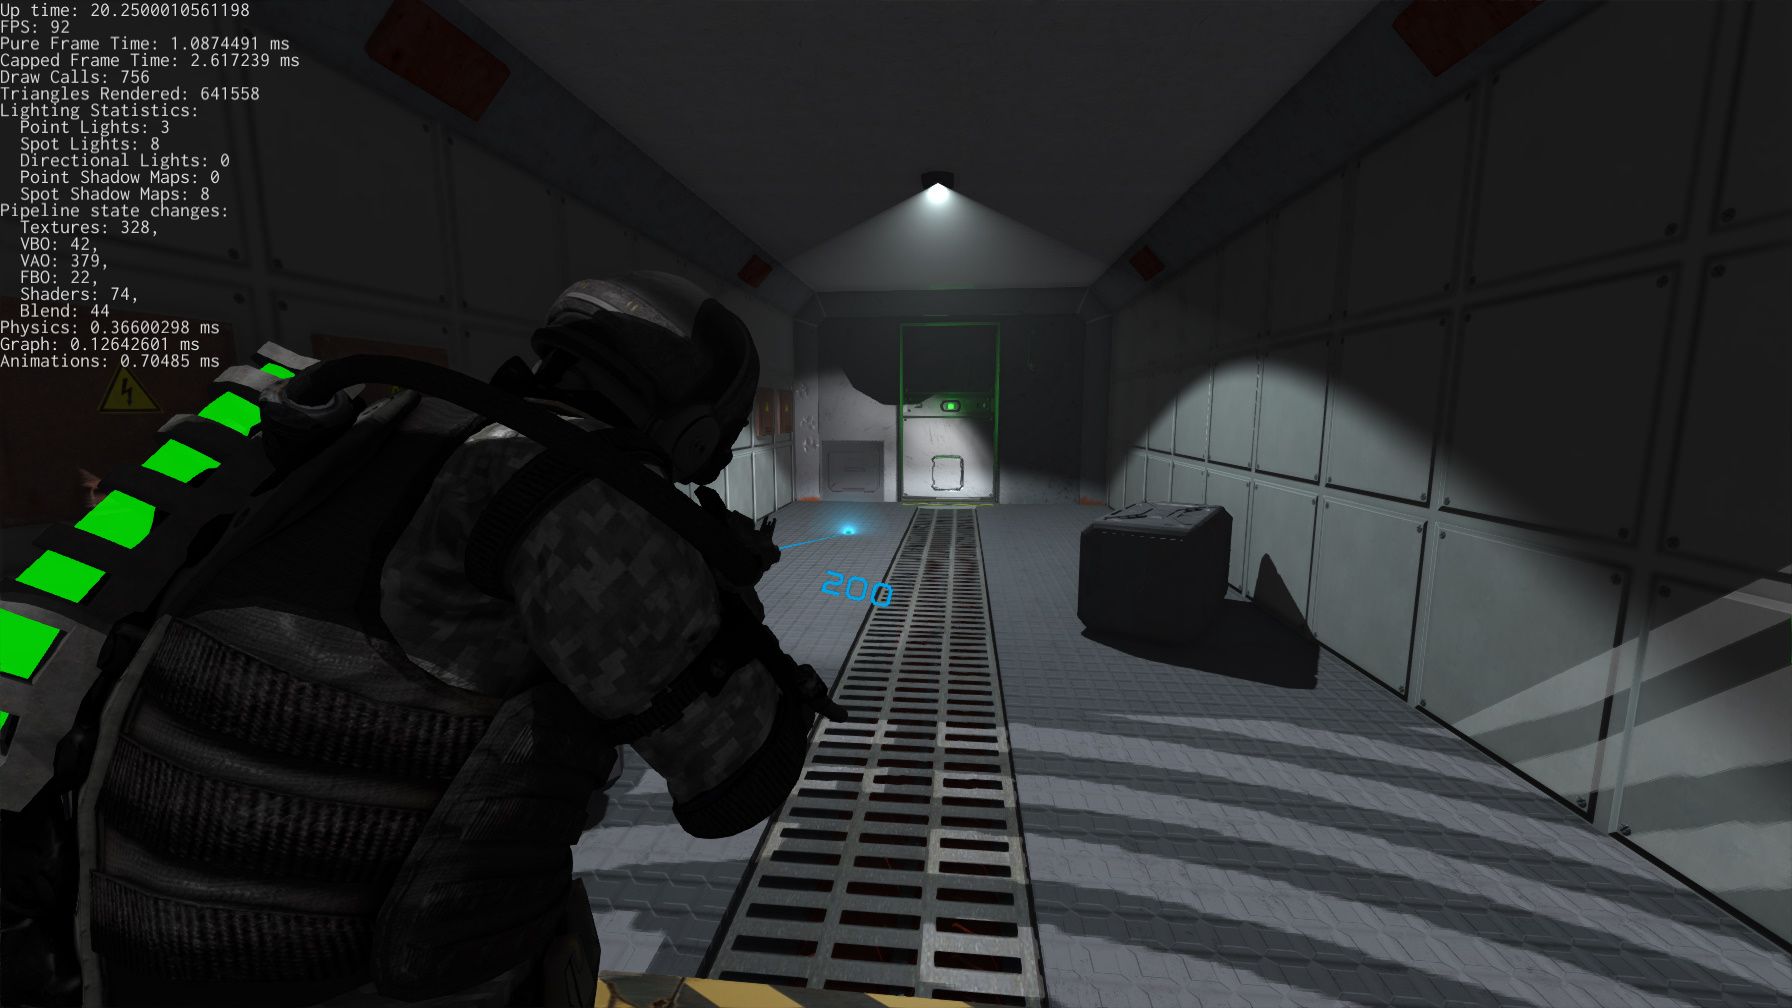
\includegraphics{images/introduction_example1.jpg}
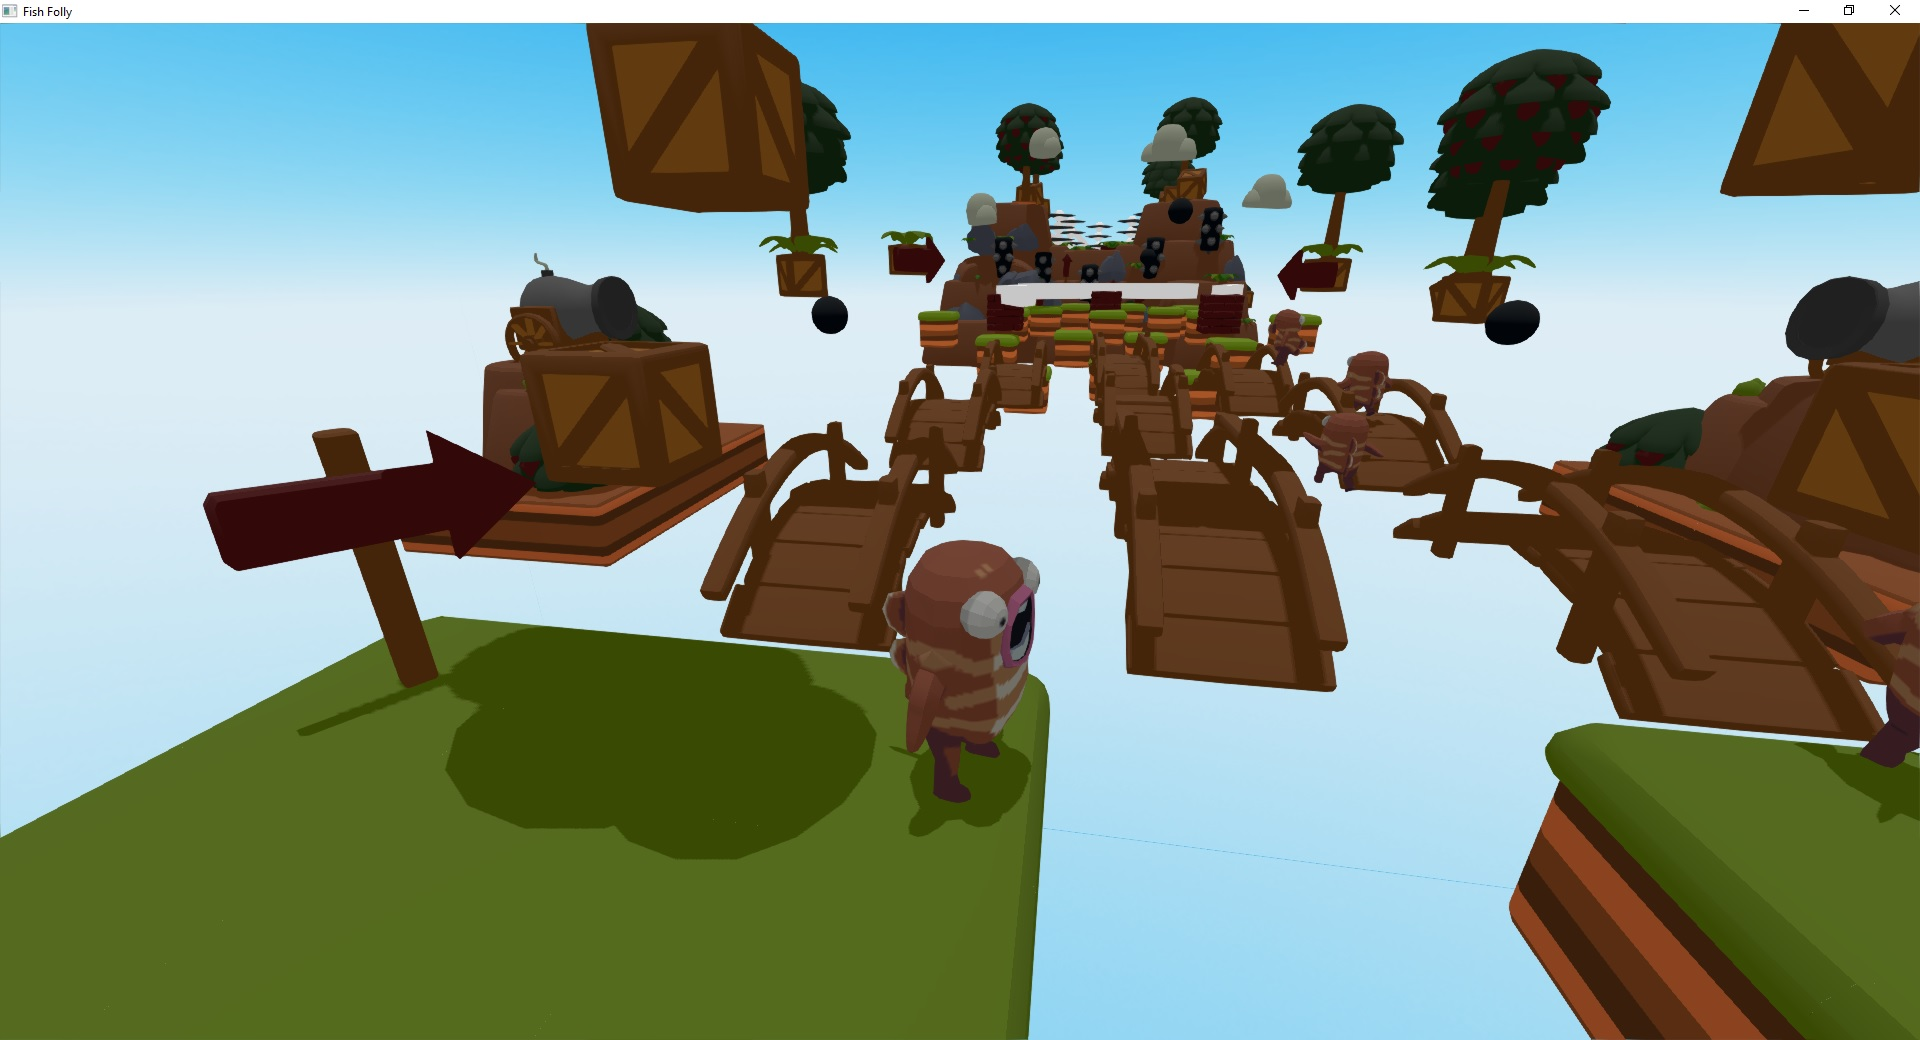
\includegraphics{images/introduction_example2.jpg}
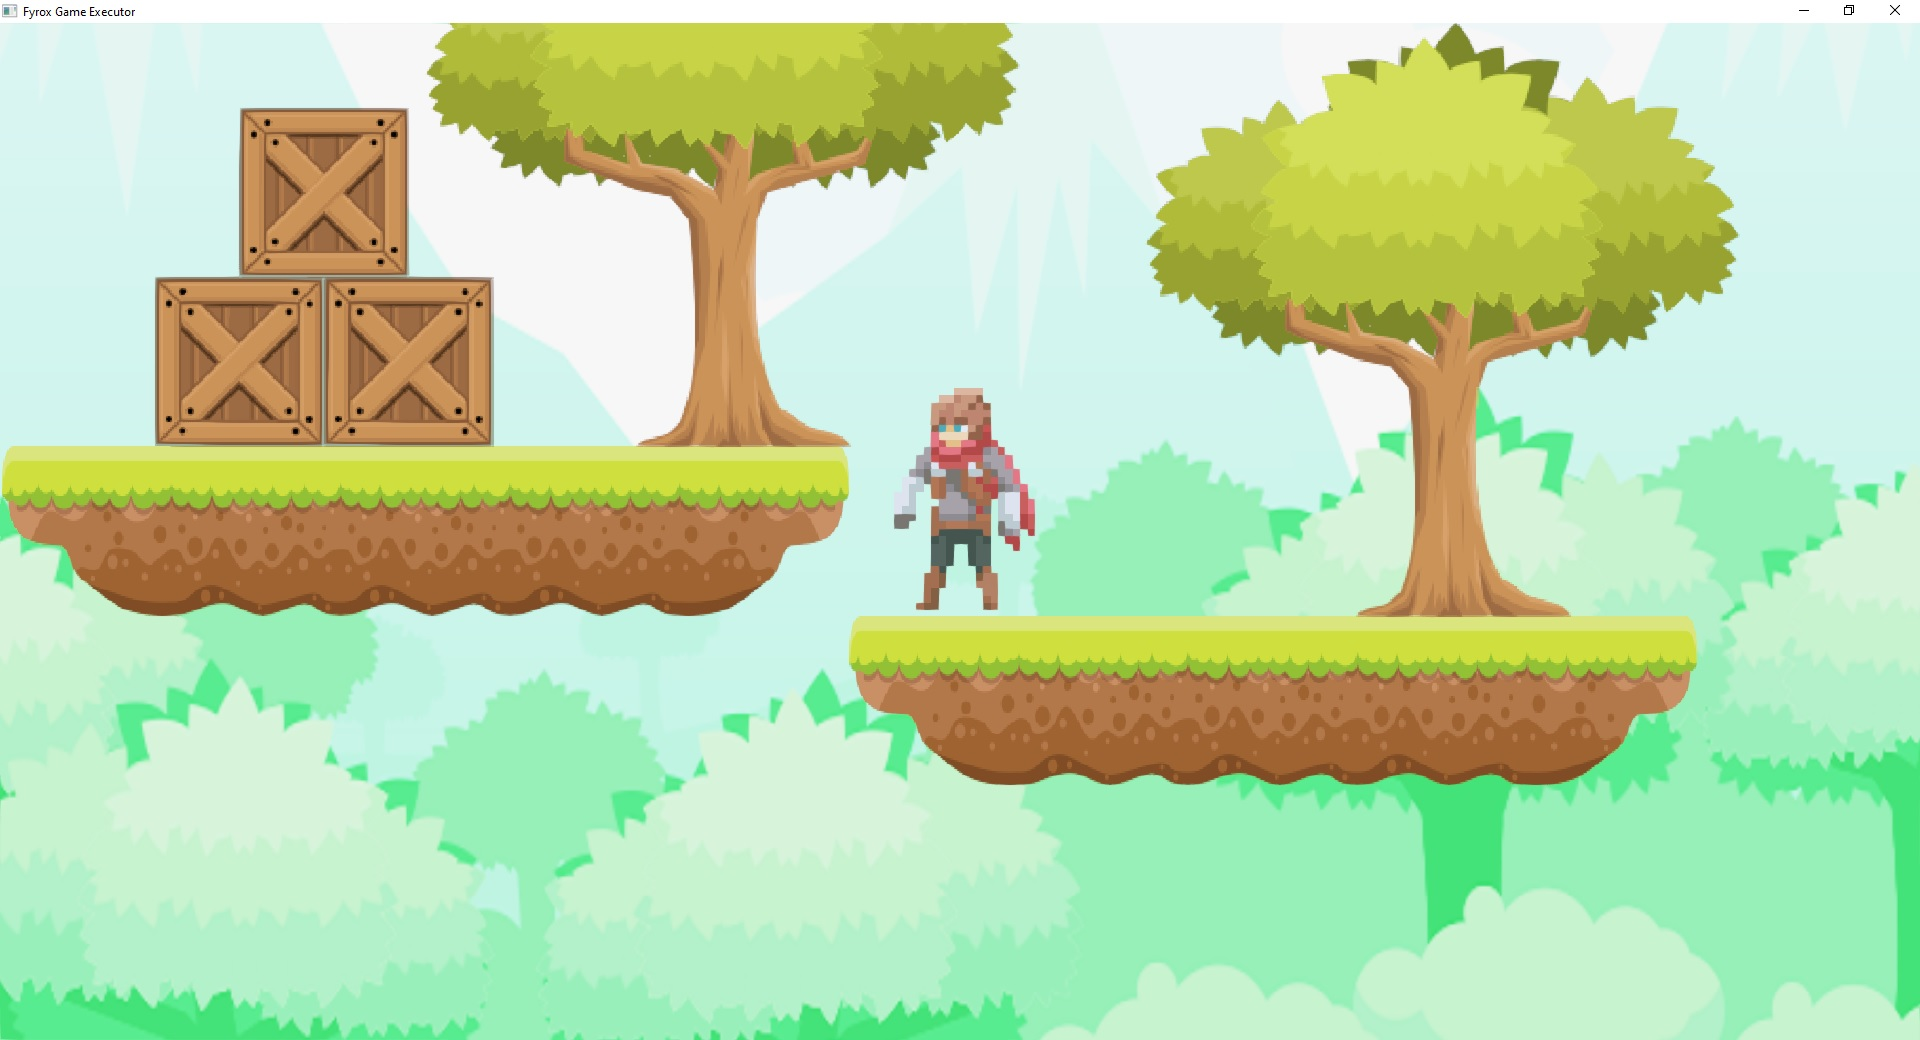
\includegraphics{images/introduction_example3.jpg}

\subsection{How does the engine work?}\label{how-does-the-engine-work}

The engine consists of two parts that you'll be actively using: the framework and the editor. The framework is a foundation of the engine, it manages rendering, sound, scripts, plugins, etc. While the editor contains lots of tools that can be used to create game worlds, manage assets, edit game objects, scripts and more.

\begin{figure}
\centering
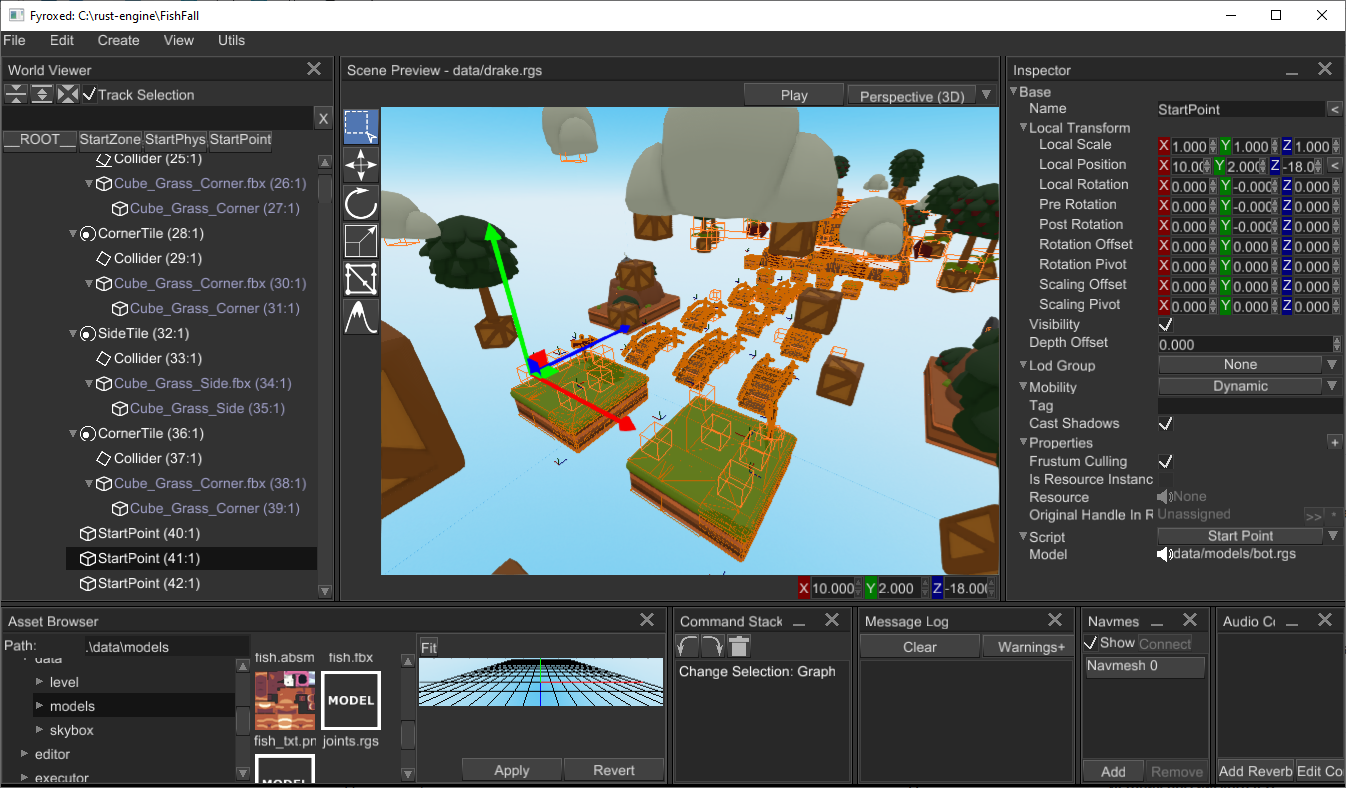
\includegraphics{images/introduction_editor.png}
\caption{Fish Folly}
\end{figure}

\subsection{Programming languages}\label{programming-languages}

Everything of your game can be written entirely in Rust, utilizing its safety guarantees as well as speed. However, it is possible to use any scripting language you want, but that's have no built-in support, and you need to implement this manually.

\subsection{Engine Features}\label{engine-features}

This is a more or less complete (yet, it can be outdated) list of engine features:

\subsubsection{General}\label{general}

\begin{itemize}
\tightlist
\item
  Exceptional safety, reliability, and speed.
\item
  PC (Windows, Linux, macOS), Android, \href{https://fyrox.rs/examples}{Web (WebAssembly) support}.
\item
  Modern, PBR rendering pipeline.
\item
  Comprehensive \href{https://docs.rs/Fyrox}{documentation}.
\item
  \href{https://fyrox-book.github.io}{Guide book}
\item
  2D support.
\item
  Integrated editor.
\item
  Fast iterative compilation.
\item
  Classic object-oriented design.
\item
  Lots of examples.
\end{itemize}

\subsubsection{Rendering}\label{rendering}

\begin{itemize}
\tightlist
\item
  Custom shaders, materials, and rendering techniques.
\item
  Physically-based rendering.
\item
  Metallic workflow.
\item
  High dynamic range (HDR) rendering.
\item
  Tone mapping.
\item
  Color grading.
\item
  Auto-exposure.
\item
  Gamma correction.
\item
  Deferred shading.
\item
  Directional light.
\item
  Point lights + shadows.
\item
  Spotlights + shadows.
\item
  Screen-Space Ambient Occlusion (SSAO).
\item
  Soft shadows.
\item
  Volumetric light (spot, point).
\item
  Batching.
\item
  Instancing.
\item
  Fast Approximate Anti-Aliasing (FXAA).
\item
  Normal mapping.
\item
  Parallax mapping.
\item
  Render in texture.
\item
  Forward rendering for transparent objects.
\item
  Sky box.
\item
  Deferred decals.
\item
  Multi-camera rendering.
\item
  Lightmapping.
\item
  Soft particles.
\item
  Fully customizable vertex format.
\item
  Compressed textures support.
\item
  High-quality mip-map on-demand generation.
\end{itemize}

\subsubsection{Scene}\label{scene}

\begin{itemize}
\tightlist
\item
  Multiple scenes.
\item
  Full-featured scene graph.
\item
  Level-of-detail (LOD) support.
\item
  GPU Skinning.
\item
  Various scene nodes:

  \begin{itemize}
  \tightlist
  \item
    Pivot.
  \item
    Camera.
  \item
    Decal.
  \item
    Mesh.
  \item
    Particle system.
  \item
    Sprite.
  \item
    Multilayer terrain.
  \item
    Rectangle (2D Sprites)
  \item
    Rigid body + Rigid Body 2D
  \item
    Collider + Collider 2D
  \item
    Joint + Joint 2D
  \end{itemize}
\end{itemize}

\subsubsection{Sound}\label{sound}

\begin{itemize}
\tightlist
\item
  \href{https://github.com/FyroxEngine/Fyrox/tree/master/fyrox-sound}{High quality binaural sound with HRTF support}.
\item
  Generic and spatial sound sources.
\item
  Built-in streaming for large sounds.
\item
  Raw samples playback support.
\item
  WAV/OGG format support.
\item
  HRTF support for excellent positioning and binaural effects.
\item
  Reverb effect.
\end{itemize}

\subsubsection{Serialization}\label{serialization}

\begin{itemize}
\tightlist
\item
  Powerful serialization system
\item
  Almost every entity of the engine can be serialized
\item
  No need to write your own serialization.
\end{itemize}

\subsubsection{Animation}\label{animation}

\begin{itemize}
\tightlist
\item
  Animation blending state machine - similar to Mecanim in Unity Engine.
\item
  Animation retargetting - allows you to remap animation from one model to another.
\end{itemize}

\subsubsection{Asset management}\label{asset-management}

\begin{itemize}
\tightlist
\item
  Advanced asset manager.
\item
  Fully asynchronous asset loading.
\item
  PNG, JPG, TGA, DDS, etc. textures.
\item
  FBX models loader.
\item
  WAV, OGG sound formats.
\item
  Compressed textures support (DXT1, DXT3, DTX5).
\end{itemize}

\subsubsection{Artificial Intelligence (AI)}\label{artificial-intelligence-ai}

\begin{itemize}
\tightlist
\item
  A* pathfinder.
\item
  Navmesh.
\item
  Behavior trees.
\end{itemize}

\subsubsection{User Interface (UI)}\label{user-interface-ui}

\begin{itemize}
\tightlist
\item
  \href{https://github.com/FyroxEngine/Fyrox/tree/master/fyrox-ui}{Advanced node-based UI} with lots of widgets
\item
  More than 32 widgets
\item
  Powerful layout system
\item
  Full TTF/OTF fonts support
\item
  Based on message passing
\item
  Fully customizable
\item
  GAPI-agnostic
\item
  OS-agnostic
\item
  Button widget
\item
  Border widget
\item
  Canvas widget
\item
  Color picker widget
\item
  Color field widget
\item
  Check box widget
\item
  Decorator widget.
\item
  Drop-down list widget
\item
  Grid widget
\item
  Image widget
\item
  List view widget
\item
  Popup widget
\item
  Progress bar widget
\item
  Scroll bar widget
\item
  Scroll panel widget
\item
  Scroll viewer widget
\item
  Stack panel widget
\item
  Tab control widget
\item
  Text widget
\item
  Text box widget
\item
  Tree widget
\item
  Window widget
\item
  File browser widget
\item
  File selector widget
\item
  Docking manager widget
\item
  NumericUpDown widget
\item
  \texttt{Vector3\textless{}f32\textgreater{}} editor widget
\item
  Menu widget
\item
  Menu item widget
\item
  Message box widget
\item
  Wrap panel widget
\item
  Curve editor widget
\item
  User defined widget
\end{itemize}

\subsubsection{Physics}\label{physics}

\begin{itemize}
\tightlist
\item
  Advanced physics (thanks to the \href{https://github.com/dimforge/rapier}{Rapier} physics engine)
\item
  Rigid bodies.
\item
  Rich set of various colliders.
\item
  Joints.
\item
  Ray cast.
\item
  Many other useful features.
\item
  2D support.
\end{itemize}

\section{System Requirements}\label{system-requirements}

As any other software, Fyrox has its own system requirements that will provide the best user experience.

\begin{itemize}
\tightlist
\item
  \textbf{CPU} - at least 2 core CPU with 1.5 GHz per each core. The more is better.
\item
  \textbf{GPU} - any relatively modern GPU with OpenGL 3.3+ support. If the editor fails to start, then it is most likely your video card does not support OpenGL 3.3+. Do \textbf{not} try to run the editor on virtual machines, pretty much all of them have rudimentary support for graphics APIs which won't let you run the editor.
\item
  \textbf{RAM} - at least 1 Gb of RAM. The more is better.
\item
  \textbf{VRAM} - at least 256 Mb of video memory. It highly depends on your game.
\end{itemize}

\subsection{Supported Platforms}\label{supported-platforms}

\begin{longtable}[]{@{}lll@{}}
\toprule\noalign{}
Platform & Engine & Editor \\
\midrule\noalign{}
\endhead
\bottomrule\noalign{}
\endlastfoot
Windows & ✅ & ✅ \\
Linux & ✅ & ✅ \\
macOS & ✅¹ & ✅ \\
WebAssembly & ✅ & ❌² \\
Android & ✅ & ❌² \\
\end{longtable}

\begin{itemize}
\tightlist
\item
  ✅ - first-class support
\item
  ❌ - not supported
\item
  ¹ - macOS suffers from bad GPU performance on Intel chipsets, M1+ works well.
\item
  ² - the editor works only on PC, it requires rich filesystem functionality as well as decent threading support.
\end{itemize}

\section{Basic concepts}\label{basic-concepts}

Let's briefly get over some basic concepts of the engine, there's not much, but all of them are crucial to understand design decisions made in the engine.

\subsection{Classic OOP}\label{classic-oop}

The engine uses somewhat classic OOP with composition over inheritance - complex objects in the engine can be constructed using simpler objects.

\subsection{Scenes}\label{scenes}

In Fyrox, you break down your game in a set of reusable scenes. Pretty much anything can be a scene: a player, a weapon, a bot, level parts, etc. Scenes can be nested one into another, this helps you to break down complex scenes into reusable parts. Scene in Fyrox is also plays a role of prefab, there's pretty much no difference between them.

\subsection{Nodes and Scene Graph}\label{nodes-and-scene-graph}

A scene is made of one or more nodes (every scene must have at least one root node, to which everything else is attached). Scene node contains specific set of properties as well as \emph{one} optional script instance which is responsible for custom game logic.

Typical structure of a scene node could be represented by the following example. The base object for every scene node is a \texttt{Base} node, it contains a transform, a list of children, etc. A more complex node, that \emph{extends} functionality of the \texttt{Base} node stores an instance of \texttt{Base} inside of them. For example, a \texttt{Mesh} node is a \texttt{Base} node \emph{plus} some specific info (a list of surfaces, material, etc.). The ``hierarchy'' depth is unlimited - a \texttt{Light} node in the engine is an enumeration of three possible types of light source. \texttt{Directional}, \texttt{Point}, and \texttt{Spot} light sources both use \texttt{BaseLight} node, which in its turn contains \texttt{Base} node inside. Graphically it can be represented like so:

\begin{Shaded}
\begin{Highlighting}[]
\NormalTok{\textasciigrave{}Point\textasciigrave{}}
\NormalTok{|\_\_ Point Light Properties (radius, etc.)}
\NormalTok{|\_\_\textasciigrave{}BaseLight\textasciigrave{}}
\NormalTok{   |\_\_ Base Light Properties (color, etc.)}
\NormalTok{   |\_\_\textasciigrave{}Base\textasciigrave{}}
\NormalTok{      |\_\_ Base Node Properties (transform, children nodes, etc.)}
\end{Highlighting}
\end{Shaded}

As you can see, this forms the nice tree (graph) that shows what the object contains. This is very natural way of describing scene nodes, it gives you the full power of building an object of any complexity.

\subsection{Plugins}\label{plugins}

Plugin is a container for ``global'' game data and logic, its main usage is to provide scripts with some data and to manage global game state.

\subsection{Scripts}\label{scripts}

Script - is a separate piece of data and logic, that can be attached to scene nodes. This is primary (but not single) way of adding custom game logic.

\section{Design Philosophy and Goals}\label{design-philosophy-and-goals}

Let's talk a bit about design philosophy and goals of the engine. Development of the engine started in the beginning
of 2019 as a hobby project to learn Rust, and it quickly showed that Rust can be a game changer in the game development
industry. Initially, the engine was just a port of \href{https://github.com/mrDIMAS/DmitrysEngine}{an engine} that is written
in C. At the beginning, it was very interesting to build such complex thing as game engine in such low level language without
any safety guarantees. After a year of development it became annoying to fix memory related issues (memory corruption,
leaks, etc.), luckily at that time Rust's popularity grew, and it showed on my radar. I (\href{https://github.com/mrDIMAS}{\citet{mrDIMAS}})
was able to port the engine to it in less than a year. Stability has improved dramatically, no more random crashes,
performance was at the same or better levels - time invested in learning new language was paid off. Development speed
does not degrade over time as it was in C, it is very easy to manage growing project.

\subsection{Safety}\label{safety}

One of the main goals in the development of the engine is to provide a high level of safety. What does this mean?
In short: protection from memory-safety related bugs. This does not include any logic errors, but when your game is free
of random crashes due to memory unsafety it is much easier to fix logic bugs, because you don't have to think about
potentially corrupted memory.

Safety also dictates the architectural design decisions of your game. The typical callback hell, that is possible to do in
many other languages, is very tedious to implement in Rust. It is possible, but it requires quite a lot of manual work
which quickly tells you that you're doing it wrong.

\subsection{Performance}\label{performance}

Game engines are usually built using system-level programming languages, which provide peak performance levels. Fyrox is not
an exception. One of its design goals is to provide high levels of performance by default, leaving an opportunity for
adding custom solutions for performance-critical places.

\subsection{Ease of use}\label{ease-of-use}

Another very important part is that the engine should be friendly to newcomers. It should lower the entry threshold, not make
it worse. Fyrox uses well known and battle-tested concepts, thus making it easier to make games with it. On the other hand,
it can still be extended with anything you need - it tries to be as good for veterans of the game industry as it is for
newcomers.

\subsection{Battle-tested}\label{battle-tested}

Fyrox has large projects built on it, which helps with understanding the real needs of a general-purpose game engine. It also helps
reveal weak spots in the design and fix them.

\section{Frequently Asked Questions}\label{frequently-asked-questions}

This chapter contains answers for frequently asked questions.

\subsection{Which graphics API does the engine use?}\label{which-graphics-api-does-the-engine-use}

Fyrox uses OpenGL 3.3 on PC and OpenGL ES 3.0 on WebAssembly. Why? Mainly due to historical reasons. Back in the day
(Q4 of 2018), there weren't any good alternatives to it with a wide range of supported platforms. For example, \texttt{wgpu}
\href{https://crates.io/crates/wgpu/0.1.0}{didn't even exist}, as its first version was released in January 2019. Other crates were taking their first baby
steps and weren't ready for production.

\subsubsection{Why not use alternatives now?}\label{why-not-use-alternatives-now}

There is no need for it. The current implementation works and is more than good enough. So instead of focusing on
replacing something that works for little to no benefit, the current focus is on adding features that are missing as
well as improving existing features when needed.

\subsection{Is the engine based on ECS?}\label{is-the-engine-based-on-ecs}

No, the engine uses a mixed composition-based, object-oriented design with message passing and other different approaches
that fit the most for a particular task. Why not use ECS for everything, though? Pragmatism. Use the right tool for the job.
Don't use a microscope to hammer nails.

\subsection{What kinds of games can I make using Fyrox?}\label{what-kinds-of-games-can-i-make-using-fyrox}

Pretty much any kind of games, except maybe games with vast open-worlds (since there's no built-in world streaming).
In general, it depends on your game development experience.

\chapter{Getting Started}\label{getting-started}

This section of the book will guide you through the basics of the engine. You will learn how to create a project, use plugins, scripts, assets, and the editor. Fyrox is a modern game engine with its own scene editor, that helps you to edit game worlds, manage assets, and many more. At the end of reading this section, you'll also learn how to manage game and engine entities, how they're structured and what are the basics of data management in the engine.

Next chapter will guide you through major setup of the engine - creating a game project using special project generator tool.

\section{Editor, Plugins and Scripts}\label{editor-plugins-and-scripts}

Every Fyrox game is just a plugin for both the engine and the editor, such approach allows the game to run from the editor and be able to edit the game entities in it. A game can define any number of scripts, which can be assigned to scene objects to run custom game logic on them. This chapter will cover how to install the engine with its platform-specific dependencies, how to use the plugins and scripting system, how to run the editor.

\subsection{Platform-specific Dependencies}\label{platform-specific-dependencies}

Before starting to use the engine, make sure all required platform-specific development dependencies are installed. If using Windows or macOS, no additional dependencies are required other than the latest Rust installed with appropriate toolchain for your platform.

\subsubsection{Linux}\label{linux}

On Linux, Fyrox needs the following libraries for development: \texttt{libxcb-shape0}, \texttt{libxcb-xfixes0}, \texttt{libxcb1}, \texttt{libxkbcommon}, \texttt{libasound2} and the \texttt{build-essential} package group.

For Debian based distros like Ubuntu, they can be installed like below:

\begin{Shaded}
\begin{Highlighting}[]
\NormalTok{sudo apt install libxcb{-}shape0{-}dev libxcb{-}xfixes0{-}dev libxcb1{-}dev libxkbcommon{-}dev libasound2{-}dev build{-}essential}
\end{Highlighting}
\end{Shaded}

For NixOS, you can use a \texttt{shell.nix} like below:

\begin{Shaded}
\begin{Highlighting}[]
\OperatorTok{\{} \VariableTok{pkgs} \OperatorTok{?} \BuiltInTok{import}\NormalTok{ \textless{}nixpkgs\textgreater{} }\OperatorTok{\{} \OperatorTok{\}} \OperatorTok{\}}\NormalTok{:}
\NormalTok{pkgs.mkShell }\KeywordTok{rec} \OperatorTok{\{}
  \VariableTok{nativeBuildInputs} \OperatorTok{=} \KeywordTok{with}\NormalTok{ pkgs.buildPackages}\OperatorTok{;} \OperatorTok{[}
\NormalTok{    pkg{-}config}
\NormalTok{    xorg.libxcb}
\NormalTok{    alsa{-}lib}
\NormalTok{    wayland}
\NormalTok{    libxkbcommon}
\NormalTok{    libGL}
  \OperatorTok{];}

  \VariableTok{shellHook} \OperatorTok{=} \KeywordTok{with}\NormalTok{ pkgs.lib}\OperatorTok{;} \StringTok{\textquotesingle{}\textquotesingle{}}
\StringTok{    export LD\_LIBRARY\_PATH=}\SpecialCharTok{$\{}\NormalTok{makeLibraryPath nativeBuildInputs}\SpecialCharTok{\}}\StringTok{:/run/opengl{-}driver/lib:$LD\_LIBRARY\_PATH}
\StringTok{  \textquotesingle{}\textquotesingle{}}\OperatorTok{;}
\OperatorTok{\}}
\end{Highlighting}
\end{Shaded}

\subsection{Quick Start}\label{quick-start}

Run the following commands to start using the editor as quickly as possible.

\begin{Shaded}
\begin{Highlighting}[]
\ExtensionTok{cargo}\NormalTok{ install fyrox{-}template}
\ExtensionTok{fyrox{-}template}\NormalTok{ init }\AttributeTok{{-}{-}name}\NormalTok{ fyrox\_test }\AttributeTok{{-}{-}style}\NormalTok{ 2d}
\BuiltInTok{cd}\NormalTok{ fyrox\_test}
\ExtensionTok{cargo}\NormalTok{ run }\AttributeTok{{-}{-}package}\NormalTok{ editor }\AttributeTok{{-}{-}release}
\end{Highlighting}
\end{Shaded}

\subsection{Project Generator}\label{project-generator}

Fyrox plugins are written in Rust, this means that if the source code of the game changes one must recompile. This architecture requires some boilerplate code. Fyrox offers a special tiny command line tool - \texttt{fyrox-template}. It helps generate all this boilerplate with a single command. Install it by running the following command:

\begin{Shaded}
\begin{Highlighting}[]
\NormalTok{cargo install fyrox{-}template}
\end{Highlighting}
\end{Shaded}

\emph{Note for Linux:} This installs it in \texttt{\$user/.cargo/bin}. If receiving errors about the \texttt{fyrox-template} command not being found, add this hidden cargo bin folder to the operating systems \texttt{\$PATH} environment variable.

Now, navigate to the desired project folder and run the following command:

\begin{Shaded}
\begin{Highlighting}[]
\NormalTok{fyrox{-}template init {-}{-}name my\_game {-}{-}style 3d}
\end{Highlighting}
\end{Shaded}

Note that unlike \texttt{cargo\ init}, this will create a new folder with the given name.

The tool accepts two arguments - a project name (\texttt{-\/-name}) and a style (\texttt{-\/-style}), which defines the contents of the default scene. After initializing the project, go to \texttt{game/src/lib.rs} - this is where the game logic is located, as you can see, the \texttt{fyrox-template} generated quite a bit of code for you. There are comments explaining what each place is for. For more info about each method, please refer \href{https://docs.rs/fyrox/latest/fyrox/plugin/trait.Plugin.html}{to the docs}.

Once the project is generated, memorize the two commands that will help run your game in different modes:

\begin{itemize}
\tightlist
\item
  \texttt{cargo\ run\ -\/-package\ editor\ -\/-release} - launches the editor with your game attached. The editor allows you to run your game from it and edit its game entities. It is intended to be used only for development.
\item
  \texttt{cargo\ run\ -\/-package\ executor\ -\/-release} - creates and runs the production binary of your game, which can be shipped (for example - to a store).
\end{itemize}

Navigate to your project's directory and run \texttt{cargo\ run\ -\/-package\ editor\ -\/-release}, after some time you should see the editor:

\begin{figure}
\centering
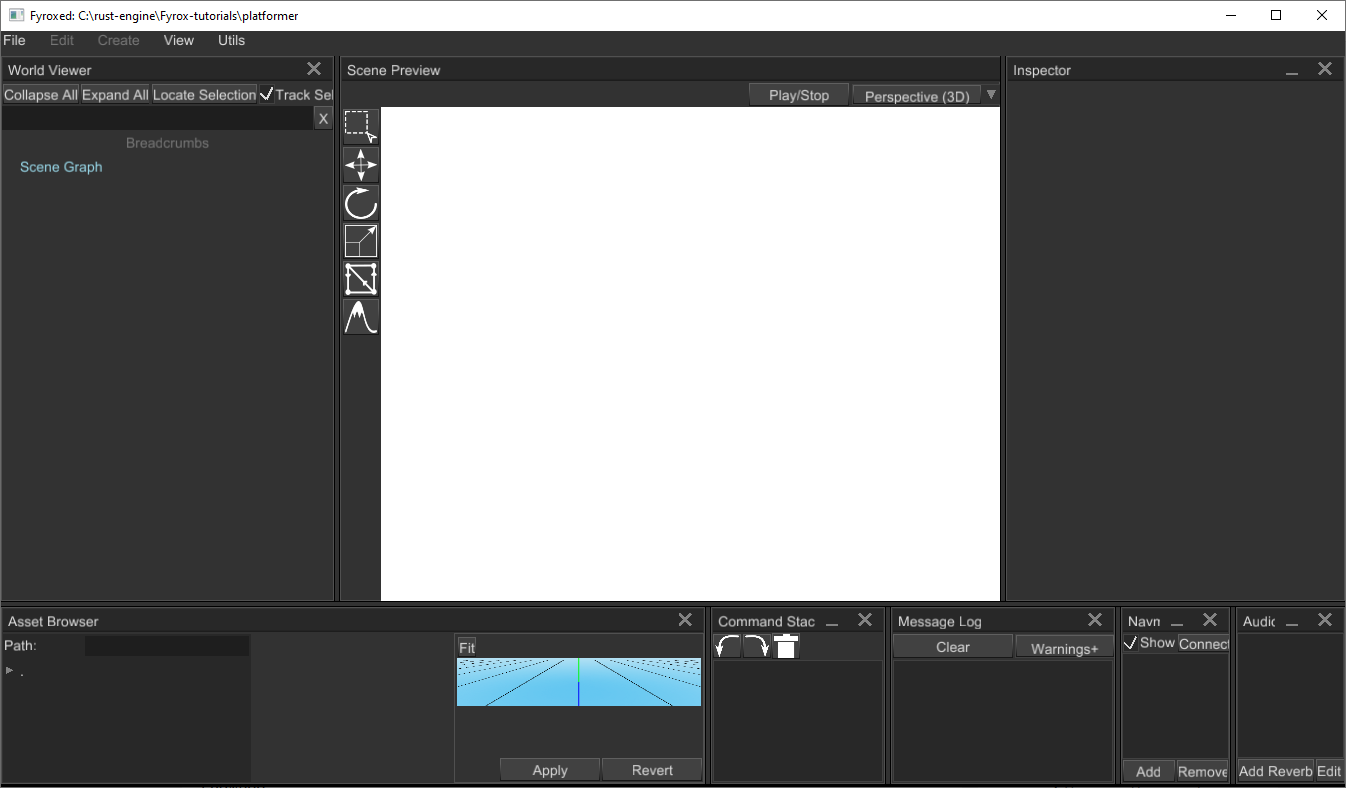
\includegraphics{images/beginning_editor.png}
\caption{editor}
\end{figure}

In the editor you can start building your game scene. \textbf{Important note:} your scene must have at least one camera, otherwise you won't see a thing. Read the next chapter to learn how to use the editor.

\subsection{Using the Latest Engine Version}\label{using-the-latest-engine-version}

Due to the nature of the software development, some bugs will inevitably sneak into the major releases, due to this, you may want to use the latest engine version from the repository on GitHub, since it is the most likely to have bugs fixed (you can also contribute by fixing any bugs you find or at least, by \href{https://github.com/FyroxEngine/Fyrox/issues}{filing an issue}).

\subsubsection{Automatic}\label{automatic}

\begin{quote}
⚠️ \texttt{fyrox-template} has special sub-command - \texttt{upgrade} to quickly upgrade to desired engine version. To upgrade to
the latest version (\texttt{nightly}) you should execute \texttt{fyrox-template\ upgrade\ -\/-version\ nightly} command in your game's
directory.
\end{quote}

There are three main variants for \texttt{-\/-version} switch:

\begin{itemize}
\tightlist
\item
  \texttt{nightly} - uses latest nightly version of the engine from GitHub directly. This is the preferable version if you want to use the latest changes and bug fixes as they release.
\item
  \texttt{latest} - uses latest stable version of the engine. This option also supports \texttt{-\/-local} key, that sets the path to the engine to \texttt{../Fyrox/fyrox} and the editor to \texttt{../Fyrox/editor}. Obviously, such path requires the engine to be located in the parent directory of your project. This option could be useful if you want to use custom version of the engine (for example, if you're developing a patch for the engine).
\item
  \texttt{major.minor.patch} - uses specific stable version from crates.io (\texttt{0.30.0} for example).
\end{itemize}

\subsubsection{Manual}\label{manual}

Engine version can also be updated manually. The first step to take is to install the latest \texttt{fyrox-template}, this can be done with a single \texttt{cargo} command:

\begin{Shaded}
\begin{Highlighting}[]
\NormalTok{cargo install fyrox{-}template {-}{-}force {-}{-}git https://github.com/FyroxEngine/Fyrox}
\end{Highlighting}
\end{Shaded}

This will ensure you're using the latest project/script template generator, which is important, since old versions of the template generator will most likely generate outdated code, no longer be compatible with the engine.

To switch existing projects to the latest version of the engine, you need to specify paths pointing to the remote repository for the \texttt{fyrox} and \texttt{fyroxed\_base} dependencies. You need to do this in the \texttt{game}, \texttt{executor}, and \texttt{editor} projects. First, open \texttt{game/Cargo.toml} and change the \texttt{fyrox} dependency to the following:

\begin{Shaded}
\begin{Highlighting}[]
\KeywordTok{[dependencies]}
\DataTypeTok{fyrox} \OperatorTok{=} \OperatorTok{\{ }\DataTypeTok{git}\OperatorTok{ =} \StringTok{"https://github.com/FyroxEngine/Fyrox"}\OperatorTok{ \}}
\end{Highlighting}
\end{Shaded}

Do the same for \texttt{executor/Cargo.toml}. The \texttt{editor} has two dependencies we need to change: \texttt{fyrox} and \texttt{fyroxed\_base}. Open the \texttt{editor/Cargo.toml} and set both dependencies to the following:

\begin{Shaded}
\begin{Highlighting}[]
\KeywordTok{[dependencies]}
\DataTypeTok{fyrox} \OperatorTok{=} \OperatorTok{\{ }\DataTypeTok{git}\OperatorTok{ =} \StringTok{"https://github.com/FyroxEngine/Fyrox"}\OperatorTok{ \}}
\DataTypeTok{fyroxed\_base} \OperatorTok{=} \OperatorTok{\{ }\DataTypeTok{git}\OperatorTok{ =} \StringTok{"https://github.com/FyroxEngine/Fyrox"}\OperatorTok{ \}}
\end{Highlighting}
\end{Shaded}

Now your game will use the latest engine and editor, but beware - new commits could bring some API breaks. You can avoid these by specifying a particular commit, just add \texttt{rev\ =\ "desired\_commit\_hash"} to every dependency like so:

\begin{Shaded}
\begin{Highlighting}[]
\KeywordTok{[dependencies]}
\DataTypeTok{fyrox} \OperatorTok{=} \OperatorTok{\{ }\DataTypeTok{git}\OperatorTok{ =} \StringTok{"https://github.com/FyroxEngine/Fyrox"}\OperatorTok{, }\DataTypeTok{rev}\OperatorTok{ =} \StringTok{"0195666b30562c1961a9808be38b5e5715da43af"}\OperatorTok{ \}}
\DataTypeTok{fyroxed\_base} \OperatorTok{=} \OperatorTok{\{ }\DataTypeTok{git}\OperatorTok{ =} \StringTok{"https://github.com/FyroxEngine/Fyrox"}\OperatorTok{, }\DataTypeTok{rev}\OperatorTok{ =} \StringTok{"0195666b30562c1961a9808be38b5e5715da43af"}\OperatorTok{ \}}
\end{Highlighting}
\end{Shaded}

To bring a local git repository of the engine to being up-to-date, just call \texttt{cargo\ update} at the root of the project's workspace. This will pull the latest changes from the remote, unless there is no \texttt{rev} specified.

Learn more about dependency paths on the official \texttt{cargo} documentation, \href{https://doc.rust-lang.org/cargo/reference/specifying-dependencies.html\#specifying-dependencies-from-git-repositories}{here}.

\subsection{Adding Game Logic}\label{adding-game-logic}

Any object-specific game logic should be added using scripts. A script is a ``container'' for data and code, that will be executed by the engine. Read the \href{../scripting/script.md}{Scripts} chapter to learn how to create, edit, and use scripts in your game.

\section{Code Hot Reloading}\label{code-hot-reloading}

Fyrox supports code hot reloading (CHR for short), which allows you to recompile the game code while the game is running. This functionality significantly reduces iteration times and allows rapid prototyping. This way, Rust becomes a sort of ``scripting'' language, but with all Rust safety and performance guarantees. CHR in action looks like this:

\subsection{How To Use}\label{how-to-use}

\begin{quote}
⚠️ If you have an existing project from one of the previous versions of the engine, the best way to add support for
CHR is to re-generate the entire project and copy all the assets and game code in the new project. CHR requires very
specific project structure and a small mistake in it could lead to incorrect behavior.
\end{quote}

CHR is quite simple to use - a project generated by \texttt{fyrox-template} already has all that is needed for hot reloading. Yet, it requires some bootstrapping to start using it. At first, you need to compile your game plugin using the following command:

\begin{Shaded}
\begin{Highlighting}[]
\NormalTok{RUSTFLAGS="{-}C prefer{-}dynamic=yes" cargo build {-}{-}package game\_dylib {-}{-}no{-}default{-}features {-}{-}features="dylib{-}engine" {-}{-}profile dev{-}hot{-}reload}
\end{Highlighting}
\end{Shaded}

This command will compile the engine DLL (\texttt{fyrox\_dylib.dll/so}) and the plugin DLL (\texttt{game\_dylib.dll/so}). Please note the mandatory environment variable \texttt{RUSTFLAGS="-C\ prefer-dynamic=yes"}. It forces the compiler to link standard library dynamically. It is very important, because if not set, the standard library will be duplicated in game plugin and engine, which will lead to subtle bugs.

\begin{quote}
⚠️ Environment variables can be set in a different ways, depending on your OS. On Linux it simply prepends the actual
command, on Windows it requires a \href{https://learn.microsoft.com/en-us/windows-server/administration/windows-commands/set_1\#examples}{separate command}.
Other OSes can have their own ways of setting environment variables.
\end{quote}

The next step is to compile the editor in CHR mode. To do that, run the following command:

\begin{Shaded}
\begin{Highlighting}[]
\NormalTok{RUSTFLAGS="{-}C prefer{-}dynamic=yes" cargo run {-}{-}package editor {-}{-}no{-}default{-}features {-}{-}features="dylib" {-}{-}profile dev{-}hot{-}reload}
\end{Highlighting}
\end{Shaded}

This command will compile the editor in CHR mode and run it. After this, all you need to do is to select build profile in the editor to be \texttt{Debug\ (HR)}:

\begin{figure}
\centering
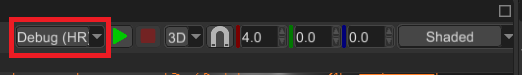
\includegraphics{images/beginning_build_profile.png}
\caption{build\_profile}
\end{figure}

Once that's done you can run your game by clicking on the green \texttt{Play} button. You can switch between CHR and normal mode (static linking) at any time. Keep in mind, that if you run the editor in CHR mode, it will also reload all changed plugins.

\subsection{Build Profiles}\label{build-profiles}

CHR uses separate build profiles: \texttt{dev-hot-reload} (no optimizations) and \texttt{release-hot-reload} (with optimizations). Separate build profiles allows you to quickly switch between statically linked plugins and code hot reloading. This could be useful if you're experiencing some issues with hot reloading (see next section for more info).

\subsection{Stability}\label{stability}

CHR is very new and experimental feature of the engine, it is based on wildly unsafe functionality which could result in memory corruption, subtle bugs, etc. If you experience weird behaviour of your game after hot reloading, run the game in normal (static linking) mode instead. Please report any bugs in the \href{https://github.com/FyroxEngine/Fyrox/issues}{issue tracker} of the engine. CHR was tested on two relatively large games - \href{https://github.com/mrDIMAS/FishFolly}{Fish Folly} and \href{https://github.com/mrDIMAS/StationIapetus}{Station Iapetus}. You can download these projects and try CHR yourself.

\subsection{Technical Details and Limitations}\label{technical-details-and-limitations}

CHR is using standard operating system (OS) mechanism of shared libraries (DLL for short). Pretty much any OS can load native code into a running process dynamically from a DLL. Any dynamically loaded library can then be unloaded from the process memory. This gives a perfect opportunity to reload game code in runtime. It may sound quite easy, but on practice there are a lot of issues.

\subsubsection{Plugin Entities and Reloading}\label{plugin-entities-and-reloading}

Plugins can supply the engine with a predefined set of entities (such as scripts, etc.). These entities are serialized into a memory blob before the plugin itself is unloaded. When all plugins are reloaded, this memory blob is used to restore the state of plugin entities. That being said, pretty much all plugin entities must be serializable (implement \texttt{Visit} trait).

\subsubsection{Trait Objects}\label{trait-objects}

Trait object are very problematic with hot reloading, because internally trait objects contains vtable with function pointers. These pointers can be easily invalidated if the plugin is unloaded. This applies even to engine trait objects, if they're created directly from the plugin side. The only way to bypass this issue is to use special methods from the engine to create its trait objects. It is possible to add a lint to clippy to check for such cases (see the respective \href{https://github.com/rust-lang/rust-clippy/issues/12819}{issue}).

\subsubsection{Dangling Objects}\label{dangling-objects}

Current plugin system tries its best to remove all plugin's entities from the engine internals before reloading plugins. However, some objects could be overlooked by this system, which could result in crash or memory corruption. Current approach of preventing to having dangling objects is based on built-in reflection system - the plugin system iterates across all fields of every object and checks its assembly name. If the assembly name match the plugin's assembly name, then this object must be deleted before the plugin is unloaded.

\subsubsection{Non-serializable Entities}\label{non-serializable-entities}

Not every object can be serialized, and in this case the current plugin system calls a special method to restore such non-serializable entities after hot reloading. Such entities could include server connections, job queues, etc.

\section{FyroxEd Overview}\label{fyroxed-overview}

FyroxEd - is the native editor of Fyrox, it is made with one purpose - to be an integrated game development environment that helps you build your game from start to finish with relatively low effort.

You'll be spending a lot of time in the editor, so you should get familiar with it and learn how to use its basic functionalities. This chapter will guide you through the basics, advanced topics will be covered in their respective chapters.

\subsection{Windows}\label{windows}

When you open the editor for the first time you may be confused by the amount of windows, buttons, lists, etc. you'll be presented with. Each window serves a different purpose, but all of them work together to help you make your game. Let's take a look at a screenshot of the editor and learn what each part of it is responsible for (please note that this can change over time, because development is quite fast and images can easily become outdated):

\begin{figure}
\centering
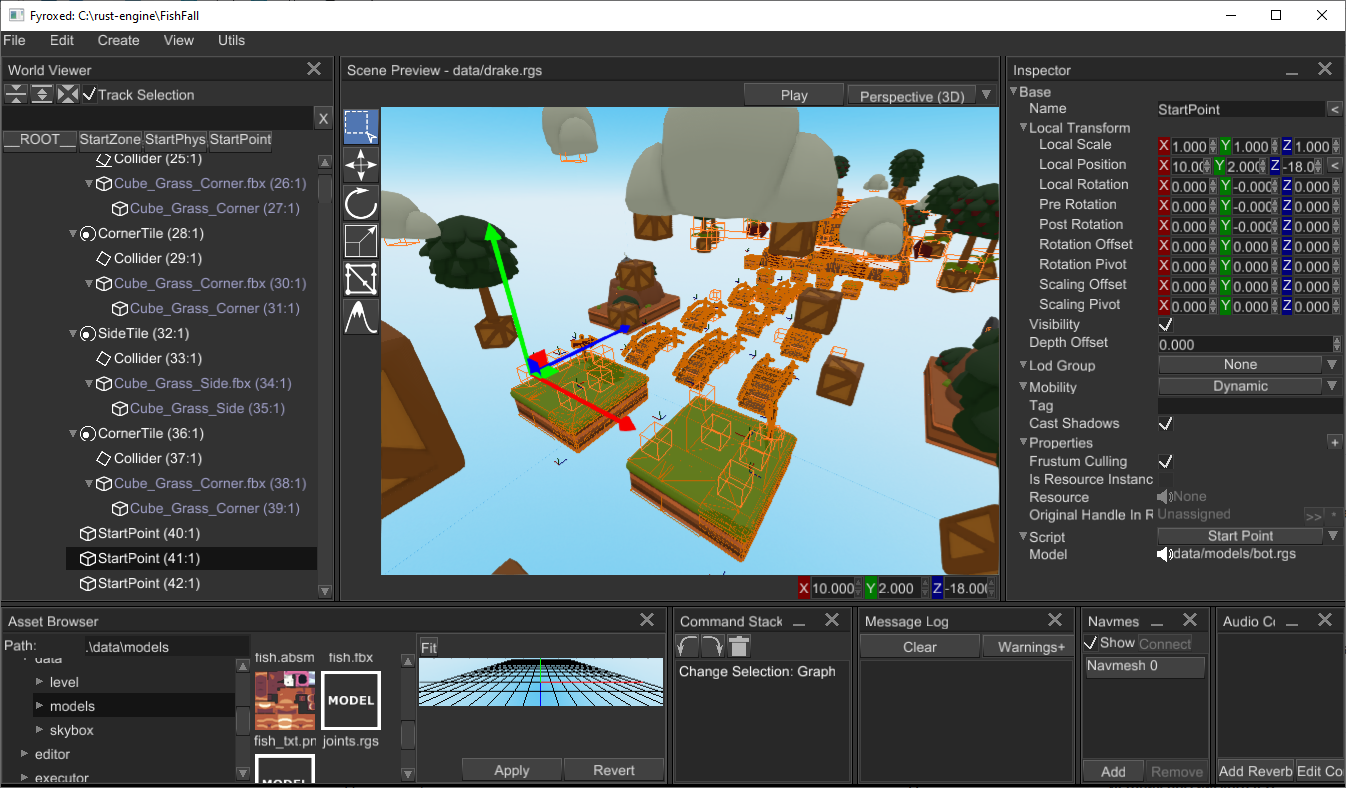
\includegraphics{./images/beginning_overview.png}
\caption{Windows}
\end{figure}

\begin{itemize}
\tightlist
\item
  \textbf{World viewer} - shows every object in the scene and their relationships. Allows inspecting and editing the contents of the scene in a hierarchical form.
\item
  \textbf{Scene preview} - renders the scene with debug info and various editor-specific objects (gizmos, entity icons, etc.). Allows you to select, move, rotate, scale, delete, etc. various entities. The \textbf{Toolbar} on its left side shows available context-dependent tools.
\item
  \textbf{Inspector} - allows you to modify various properties of the selected object.
\item
  \textbf{Message Log} - displays important messages from the editor.
\item
  \textbf{Navmesh Panel} - allows you to create, delete, and edit navigational meshes.
\item
  \textbf{Command Stack} - displays your most recent actions and allows you to undo or redo their changes.
\item
  \textbf{Asset Browser} - allows you to inspect the assets of your game and to instantiate resources in the scene, among other things.
\item
  \textbf{Audio Context} - allows you to edit the settings of the scene's sound context (global volume, available audio buses, effects, etc.)
\end{itemize}

\subsection{Creating or loading a Scene}\label{creating-or-loading-a-scene}

FyroxEd works with scenes - a scene is a container for game entities, you can create and edit one scene at a time. You must have a scene loaded to begin working with the editor. To create a scene go to \texttt{File\ -\textgreater{}\ New\ Scene}.

To load an existing scene, go to \texttt{File\ -\textgreater{}\ Load} and select the desired scene through the file browser. Recently opened scenes can be loaded more quickly by going to \texttt{File\ -\textgreater{}\ Recent\ Scenes} and selecting the desired one.

\subsection{Populating a Scene}\label{populating-a-scene}

A scene can contain various game entities. There are two equivalent ways of creating these:

\begin{itemize}
\tightlist
\item
  By going to \texttt{Create} in the main menu and selecting the desired entity from the drop down.
\item
  By right-clicking on a game entity in the \texttt{World\ Viewer} and selecting the desired entity from the \texttt{Create\ Child} sub-menu.
\end{itemize}

Complex objects usually made in 3D modelling software (Blender, 3Ds Max, Maya, etc.) can be saved in various formats. Fyrox supports FBX format, which is supported by pretty much any 3D modelling software. You can instantiate such objects by simply dragging the one you want and dropping it on the \texttt{Scene\ Preview}. While dragging it, you'll also see a preview of the object.

You can do the same with other scenes made in the editor (\texttt{rgs} files), for example, you can create a scene with a few objects in it with some scripts and re-use them within other scenes. Such scenes are called \href{../scene/prefab.md}{prefabs}.

\subsection{Saving a Scene}\label{saving-a-scene}

To save your work, go to \texttt{File\ -\textgreater{}\ Save}. If you're saving a new scene, the editor will ask you to specify a file name and a path to where the scene will be saved. Scenes loaded from a file will automatically be saved to the path they were loaded from.

\subsection{Undoing and redoing}\label{undoing-and-redoing}

FyroxEd remembers your actions and allows you to undo and redo the changes done by these. You can undo or redo changes by either going to \texttt{Edit\ -\textgreater{}\ Undo/Redo} or through the usual shortcuts: \texttt{Ctrl+Z} - to undo, \texttt{Ctrl+Y} - to redo.

\subsection{Controls}\label{controls}

There are number of control keys that you'll be using most of the time, pretty much all of them work in the \texttt{Scene\ Preview} window:

\subsubsection{Editor camera movement}\label{editor-camera-movement}

Click and hold \texttt{{[}Right\ Mouse\ Button{]}} within the \texttt{Scene\ Preview} window to enable the movement controls:
- \texttt{{[}W{]}{[}S{]}{[}A{]}{[}D{]}} - Move camera forward/backward/left/right
- \texttt{{[}Space{]}{[}Q{]}/{[}E{]}} - Raise/Lower Camera
- \texttt{{[}Ctrl{]}} - Speed up
- \texttt{{[}Shift{]}}- Slowdown
\#\#\#\# Others
- \texttt{{[}Left\ Mouse\ Button{]}} - Select
- \texttt{{[}Middle\ Mouse\ Button{]}} - Pan camera in viewing plane
- \texttt{{[}1{]}} - Select interaction mode
- \texttt{{[}2{]}} - Move interaction mode
- \texttt{{[}3{]}} - Scale interaction mode
- \texttt{{[}4{]}} - Rotate interaction mode
- \texttt{{[}5{]}} - Navigational mesh editing mode
- \texttt{{[}6{]}} - Terrain editing interaction mode
- \texttt{{[}Ctrl{]}+{[}Z{]}} - Undo
- \texttt{{[}Ctrl{]}+{[}Y{]}} - Redo
- \texttt{{[}Delete{]}} - Delete current selection.

\subsection{Play Mode}\label{play-mode}

One of the key features of the editor is that it allows you to run your game from it in a separate process. Use the \texttt{Play/Stop} button at the top of the \texttt{Scene\ Preview} window to enter or leave Play Mode. Keep in mind, that the editor UI will be locked while you're in Play Mode.

Play Mode can be activated only for projects made with the \texttt{fyrox-template} (or for projects with a similar structure). The editor calls \texttt{cargo} commands to build and run your game in a separate process. Running the game in a separate process ensures that the editor won't crash if your game does, it also provides excellent isolation between the game and the editor, not giving a chance to break the editor by running the game.

\subsection{Additional Utilities}\label{additional-utilities}

There are also number of powerful utilities that will make your life easier, they can be found under the \texttt{Utils} section of the main menu:

\begin{itemize}
\tightlist
\item
  Curve Editor - allows you to create and edit curve resources to make complex laws for game parameters.
\item
  Path Fixer - helps you fix incorrect resource references in your scenes.
\end{itemize}

\section{Scene and Scene Graph}\label{scene-and-scene-graph}

When you're playing a game, you often see various objects scattered around the screen, all of them are forming a \emph{scene}. A scene is just a set of a variety objects, as in many other game engines, Fyrox allows you to create multiple scenes for multiple purposes, for example, one scene could be used for a menu, a bunch of others for game levels, and another one for an ending screen. Scenes can also be used to create a source of data for other scenes, such scenes are called \emph{prefabs}. Scenes can also be rendered in a texture, which can be used in other scenes - this way you can create interactive screens that show other places.

While playing games, you may have noticed that some objects behaves as if they were linked to other objects, for example, a character in a role-playing game could carry a sword. While the character holds the sword, it is linked to his arm. Such relations between the objects can be presented by a graph structure.

Simply speaking, a graph is a set of objects with hierarchical relationships between each object. Each object in the graph is called a \emph{node}. In the example with the sword and the character, the sword is a \emph{child} node of the character, and the character is a \emph{parent} node of the sword (here we ignore the fact that in reality, character models usually contain complex skeletons, with the sword actually being attached to one of the hands' bones, not to the character).

You can change the hierarchy of nodes in the editor using a simple drag'n'drop functionality in the \texttt{World\ Viewer} - drag a node onto some other node, and it will attach itself to it.

\subsection{Building Blocks or Scene Nodes}\label{building-blocks-or-scene-nodes}

The engine offers various types of ``building blocks'' for your scene, each such block is called a \emph{scene node}.

\begin{itemize}
\tightlist
\item
  \href{../scene/base_node.md}{Base} - stores hierarchical information (a handle to the parent node and handles to children nodes), local and global transform, name, tag, lifetime, etc. It has self-describing name - it's used as a base node for every other scene node via composition.
\item
  \href{../scene/mesh_node.md}{Mesh} - represents a 3D model. This one of the most commonly used nodes in almost every game. Meshes can be easily created either programmatically, or be made in some 3D modelling software, such as Blender, and then loaded into the scene.
\item
  \href{../scene/light_node.md}{Light} - represents a light source. There are three types of light sources:

  \begin{itemize}
  \tightlist
  \item
    \textbf{Point} - emits light in every direction. A real-world example would be a light bulb.
  \item
    \textbf{Spot} - emits light in a particular direction, with a cone-like shape. A real-world example would be a flashlight.
  \item
    \textbf{Directional} - emits light in a particular direction, but does not have position. The closest real-world example would be the Sun.
  \end{itemize}
\item
  \href{../scene/camera_node.md}{Camera} - allows you to see the world. You must have at least one camera in your scene to be able to see anything.
\item
  \href{../scene/sprite_node.md}{Sprite} - represents a quad that always faces towards a camera. It can have a texture and size and can also can be rotated around the ``look'' axis.
\item
  \href{../scene/particle_system_node.md}{Particle system} - allows you to create visual effects using a huge set of small particles. It can be used to create smoke, sparks, blood splatters, etc.
\item
  \href{../scene/terrain_node.md}{Terrain} - allows you to create complex landscapes with minimal effort.
\item
  \href{../scene/decal_node.md}{Decal} - paints on other nodes using a texture. It is used to simulate cracks in concrete walls, damaged parts of the road, blood splatters, bullet holes, etc.
\item
  \href{../physics/rigid_body.md}{Rigid Body} - a physical entity that is responsible for the dynamic of the rigid. There is a special variant for 2D - \texttt{RigidBody2D}.
\item
  \href{../physics/collider.md}{Collider} - a physical shape for a rigid body. It is responsible for contact manifold generation, without it, any rigid body will not participate in simulation correctly, so every rigid body must have at least one collider. There is a special variant for 2D - \texttt{Collider2D}.
\item
  \href{../physics/joint.md}{Joint} - a physical entity that restricts motion between two rigid bodies. It has various amounts of degrees of freedom depending on the type of the joint. There is a special variant for 2D - \texttt{Joint2D}.
\item
  \href{../scene/rectangle.md}{Rectangle} - a simple rectangle mesh that can have a texture and a color. It is a very simple version of a Mesh node, yet it uses very optimized renderer, that allows you to render dozens of rectangles simultaneously. This node is intended for use in \textbf{2D games} only.
\item
  \href{../sound/sound.md}{Sound} - a sound source universal for 2D and 3D. Spatial blend factor allows you to select a proportion between 2D and 3D.
\item
  Listener - an audio receiver that captures the sound at a particular point in your scene and sends it to an audio context for processing and outputting to an audio playback device.
\item
  Animation Player - a container for multiple animations. It can play animations made in the \href{../animation/anim_editor.md}{animation editor} and apply animation poses to respective scene nodes.
\item
  Animation Blending State Machine - a state machine that mixes multiple animations from multiple states into one; each state is backed by one or more animation playing or blending nodes. See its \href{../animation/absm_editor.md}{respective chapter} for more info.
\end{itemize}

Every node can be created either in the editor (through \texttt{Create} on the main menu, or through \texttt{Add\ Child} after right-clicking on a game entity) or programmatically via their respective node builder (see \href{https://docs.rs/fyrox/latest/fyrox/scene/index.html}{API docs} for more info). These scene nodes allow you to build almost any kind of game. It is also possible to create your own types of nodes, but that is an advanced topic, which is covered in a \href{../scene/custom_node.md}{future chapter}.

\subsection{Local and Global Coordinates}\label{local-and-global-coordinates}

A graph describes your scene in a very natural way, allowing you think in terms of relative and absolute coordinates when working with \emph{scene nodes}.

A scene node has two kinds of transform - a local and global. The local transform defines where the node is located relative to its origin, its scale as a percentage, and its rotation around any arbitrary axis.The global transform is almost the same, but it also includes the whole chain of transforms of the parent nodes. Going back to the example of the character and the sword, if the character moves, and by extension the sword, the global transform of the sword will reflect the changes made to the character position, yet its local transform will not, since that represents the sword's position's relative to the character's, which didn't change.

This mechanism is very simple, yet powerful. The full grace of it unfolds when you're working with 3D models with skeletons. Each bone in a skeleton has its parent and a set of children, which allows you to rotate, translate, or scale them to animate your entire character.

\section{Assets}\label{assets}

Pretty much every game depends on various assets, such as 3D models, textures, sounds, etc. Fyrox has its own assets pipeline made to make your life easier.

\subsection{Asset Types}\label{asset-types}

The engine offers a set of assets that should cover all of your needs:

\begin{itemize}
\tightlist
\item
  \href{../resources/model.md}{Models} - are a set of objects. They can be a simple 3D model (barrels, bushes, weapons,
  etc.) or complex scenes with lots of objects and possibly other model instances. Fyrox supports two main formats:
  FBX - which can be used to import 3D models, RGS - which are scenes made in FyroxEd. RGS models are special, as they can be
  used as \emph{hierarchical prefabs}.
\item
  \href{../resources/texture.md}{Textures} - are images used to add graphical details to objects. The
  engine supports multiple texture formats, such as PNG, JPG, BMP, etc. Compressed textures in DDS format are also supported.
\item
  \href{../resources/sound.md}{Sound buffers} - are data buffers for sound sources. Fyrox supports WAV and OGG formats.
\item
  \href{../resources/curve.md}{Curves} - are parametric curves. They're used to create complex functions for numeric parameters.
  They can be made in the \texttt{Curve\ Editor} (\texttt{Utils\ -\textgreater{}\ Curve\ Editor})
\item
  \href{../sound/hrtf.md}{HRIR Spheres} - head-related impulse response collection used for head-related transfer function
  in the HRTF sound rendering.
\item
  \href{../ui/font.md}{Fonts} - arbitrary TTF/OTF fonts.
\item
  \href{../rendering/materials.md}{Materials} - materials for rendering.
\item
  \href{../rendering/shaders.md}{Shaders} - shaders for rendering.
\item
  It is also possible to create custom assets. See \href{../resources/custom.md}{respective chapter} for more info.
\end{itemize}

\subsection{Asset Management}\label{asset-management-1}

Asset management is performed from the \texttt{Asset\ Browser} window in the editor, you can select an asset, preview it, and edit its import options. Here's a screenshot of the asset browser with a texture selected:

\begin{figure}
\centering
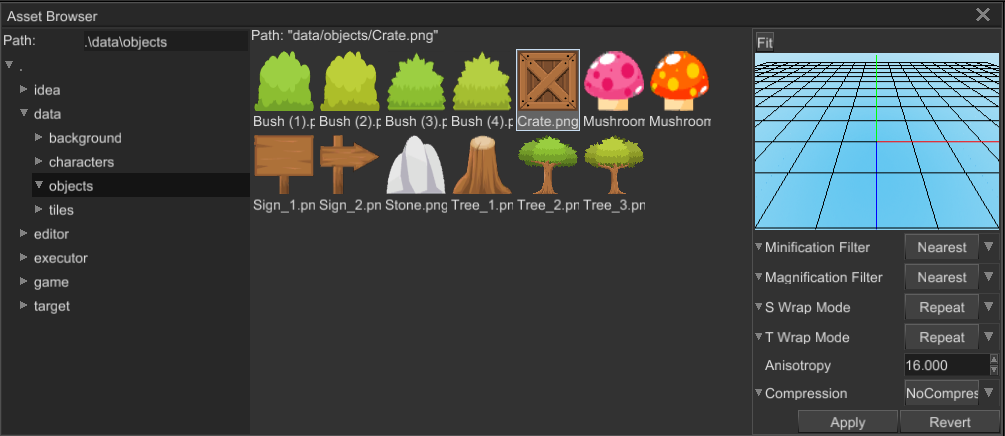
\includegraphics{images/beginning_assets.png}
\caption{asset browser}
\end{figure}

The most interesting part here is the import options section under the previewer. It allows you to set asset-specific import options and apply them. Every asset has its own set of import options. See their respective asset page from the section above to learn what each import option is for.

\subsection{Asset Instantiation}\label{asset-instantiation}

Some asset types can be instantiated in scenes; for now, you can only create direct instances from models. This is done by simply dragging the model you want to instantiate and dropping it on the \texttt{Scene\ Preview}. While dragging it, you'll also see a preview of the model.

\begin{figure}
\centering
\includegraphics{images/preview.gif}
\caption{preview}
\end{figure}

The maximum amount of asset instances is not limited by the engine but it is by the memory and CPU resources of your PC. Note that the engine does try to reuse data across instances as much as possible.

You can also instantiate assets dynamically from your code. Here's an example of that for a Model:

\begin{Shaded}
\begin{Highlighting}[]
\NormalTok{\{\{\#include ../code/snippets/src/resource/mod.rs:instantiate\_model\}\}}
\end{Highlighting}
\end{Shaded}

This is very useful with prefabs that you may want to instantiate in a scene at runtime.

\subsection{Loading Assets}\label{loading-assets}

Usually, there is no need to manually handle the loading of assets since you have the editor to help with that - just create a scene with all the required assets. However, there are times when you may need to instantiate some asset dynamically, for example, a bot prefab. For these cases, you can use the \texttt{ResourceManager::request\textless{}T\textgreater{}} method with the appropriate type, such as \texttt{Model}, \texttt{Texture}, \texttt{SoundBuffer}, etc.

\section{Data Management}\label{data-management}

The engine uses pools to store most objects (scene nodes in a graph, animations in an animation player, sound sources in an audio context, etc.). Since you'll use them quite often, reading and understanding this chapter is recommended.

\subsection{Motivation}\label{motivation}

Rust ownership system and borrow checker, in particular, dictate the rules of data management. In game development, you often have the need to reference objects from other objects. In languages like C, this is usually achieved by simply storing a raw pointer and calling it a day. That works, yet it's remarkably unsafe - you risk either forgetting to destroy an object and leaking memory or destroying an object still being referenced and then trying to access deallocated memory. Other languages, like C++, allow you to store \emph{shared pointers} to your data, which by keeping a reference count, ensures the previous doesn't happen at the cost of a, most often, negligible overhead. Rust counts with smart pointers similar to this, though not without their limitations. There is the \texttt{Rc/Arc} - they function like \emph{shared pointers}, except they don't allow mutating their content, only reading it. If you want mutability, you use either a \texttt{RefCell} for a single-threaded environment, or a \texttt{Mutex} for a multithreaded environment. That is where the problems begin. For types such as \texttt{Rc\textless{}RefCell\textgreater{}} or \texttt{Arc\textless{}Mutex\textgreater{}}, Rust enforces its borrowing rules at runtime, which are unlimited readers but a single writer. Any attempt to borrow mutably more than once at a time will lead to a runtime error.

Another problem with these shared references is that is very easy to accidentally create cyclical references that prevent objects from ever being destroyed. While the previous could be lived with, the last problem is especially severe in the case of games: the overhead of runtime checks. In the case of a \texttt{Rc\textless{}RefCell\textgreater{}}, it is a single reference counter for given accesses to the data, but in the case of a \texttt{Arc\textless{}Mutex\textgreater{}}, it is a mutex lock.

The solution to these problems is far from ideal; it certainly has its own downfalls. Instead of scattering objects across memory and then having to manage the lifetime of each of them through reference counting, we can store all of the objects in a single and contiguous memory block and then use indices to access each object. Such a structure is called a pool.

\subsection{Technical Details}\label{technical-details}

A pool is an efficient method of data management. A pool is a vector with entries that can be either vacant or occupied. Each entry, regardless of its status, also stores a number called a \emph{generation} number. This is used to understand whether an entry has changed over time or not. When an entry is reused, its generation number is increased, rendering all previously created handles leading to the entry invalid. This is a simple and efficient algorithm for tracking the lifetime of objects.

To access the data in the entries, the engine uses the previously mentioned \emph{handles}. A handle is a pair of the index of an entry
and a generation number. When you put an object in the pool, this gives you the handle that leads to the object, as well as the
entry's current generation number. The number remains valid until you ``free'' the object, which makes the entry vacant again.

\subsection{Advantages}\label{advantages}

\begin{itemize}
\tightlist
\item
  Since a pool is a contiguous memory block, it is far more CPU cache-friendly. This reduces the occurrences of CPU cache misses, which makes accesses to data blazingly fast.
\item
  Almost every entity in Fyrox lives on its own pool, which makes it easy to create data structures
  like graphs, where nodes refer to other nodes. In this case, nodes simply need to store a handle to refer to other nodes.
\item
  Simple lifetime management. There is no way to leak memory since cross-references can only be done via handles.
\item
  Fast random access with a constant complexity.
\item
  Handles are the same size as a pointer on a 64-bit architecture, just 8 bytes.
\end{itemize}

\subsection{Disadvantages}\label{disadvantages}

\begin{itemize}
\tightlist
\item
  Pools can contain lots of gaps between currently used memory, which may lead to less efficient memory usage.
\item
  Handles are sort of weak references, but worse. Since they do not own any data nor even point to their data, you need a reference to its pool instance in order to borrow the data a handle leads to.
\item
  Handles introduce a level of indirection that can hurt performance in places with high loads that require random access, though this is not too significant as random access is already somewhat slow because of potential CPU cache misses.
\end{itemize}

\subsection{Usage}\label{usage}

You'll use \texttt{Handle} \emph{a lot} while working with Fyrox. So where are the main usages of pools and handles? The largest is in a \href{../scene/graph.md}{scene graph}. This stores all the nodes in a pool and gives handles to each node. Each scene node stores a handle to their parent node and a set of handles to their children nodes. A scene graph automatically ensures that such handles are valid. In \href{../scripting/script.md}{scripts}, you can also store handles to scene nodes and assign them in the editor. \href{../animation/animation.md}{Animation} is another place that stores handles to animated scene nodes. \href{../animation/blending.md}{Animation Blending State Machine} stores its own state graph using a pool; it also takes handles to animations from an animation player in a scene.

And the list could keep going for a long time. This is why you need to understand the basic concepts of data management, as to efficiently and fearlessly use Fyrox.

\subsection{Borrowing}\label{borrowing}

Once an object is placed in a pool, you have to use its respective handle to get a reference to it. This can be done with either \texttt{pool.borrow(handle)} or \texttt{pool.borrow\_mute(handle)}, or by using the \texttt{Index} trait: \texttt{pool{[}handle{]}}. Note that these methods panic when the handle given is invalid. If you want to be safe, use the \texttt{try\_borrow(handle)} or \texttt{try\_borrow\_mut(handle)} method.

\begin{Shaded}
\begin{Highlighting}[]
\NormalTok{\# extern crate fyrox;}
\NormalTok{\# use fyrox::core::pool::Pool;}
\NormalTok{\#}
\NormalTok{\# fn main() \{}
\NormalTok{let mut pool = Pool::\textless{}u32\textgreater{}::new();}
\NormalTok{let handle = pool.spawn(1);}

\NormalTok{let obj = pool.borrow\_mut(handle);}
\NormalTok{*obj = 11;}

\NormalTok{let obj = pool.borrow(handle);}
\NormalTok{assert\_eq!(*obj, 11);}
\NormalTok{\# \}}
\end{Highlighting}
\end{Shaded}

\subsection{Freeing}\label{freeing}

You can extract an object from a pool by calling \texttt{pool.free(handle)}. This will give you the object back and make all current handles to it invalid.

\begin{Shaded}
\begin{Highlighting}[]
\NormalTok{\# extern crate fyrox;}
\NormalTok{\# use fyrox::core::pool::Pool;}
\NormalTok{\#}
\NormalTok{\# fn main() \{}
\NormalTok{let mut pool = Pool::\textless{}u32\textgreater{}::new();}
\NormalTok{let handle = pool.spawn(1);}

\NormalTok{pool.free(handle);}

\NormalTok{let obj = pool.try\_borrow(handle);}
\NormalTok{assert\_eq!(obj, None);}
\NormalTok{\# \}}
\end{Highlighting}
\end{Shaded}

\subsection{Take and Reserve}\label{take-and-reserve}

Sometimes you may want to temporarily extract an object from a pool, do something with it, and then put it back, yet not want to break every handle to the object in the process. There are three methods for this:

\begin{enumerate}
\def\labelenumi{\arabic{enumi})}
\tightlist
\item
  \texttt{take\_reserve} + \texttt{try\_take\_reserve} - moves an object out of the pool but leaves the entry in an occupied state. This function returns a tuple with two values \texttt{(Ticket\textless{}T\textgreater{},\ T)}. The latter one being your object, and the former one being a wrapper over its index that allows you to return the object once you're done with it. This is called a ticket. Note that attempting to borrow a moved object will cause a panic!
\item
  \texttt{put\_back} - moves the object back using the given ticket. The ticket contains information about where in the pool to return the object to.
\item
  \texttt{forget\_ticket} - makes the pool entry vacant again. Useful in cases where you move an object out of the pool, and then decide you won't return it. If this is the case, you \textbf{must} call this method, otherwise, the corresponding entry will remain unusable.
\end{enumerate}

Reservation example:

\begin{Shaded}
\begin{Highlighting}[]
\NormalTok{\# extern crate fyrox;}
\NormalTok{\# use fyrox::core::pool::Pool;}
\NormalTok{\#}
\NormalTok{\# fn main() \{}
\NormalTok{let mut pool = Pool::\textless{}u32\textgreater{}::new();}
\NormalTok{let handle = pool.spawn(1);}

\NormalTok{let (ticket, ref mut obj) = pool.take\_reserve(handle);}

\NormalTok{*obj = 123;}

\NormalTok{// Attempting to fetch while there is an existing reservation, will fail.}

\NormalTok{let attempt\_obj = pool.try\_borrow(handle);}
\NormalTok{assert\_eq!(attempt\_obj, None);}

\NormalTok{// Put the object back, allowing borrowing again.}

\NormalTok{pool.put\_back(ticket, *obj);}

\NormalTok{let obj = pool.borrow(handle);}

\NormalTok{assert\_eq!(obj, \&123);}
\NormalTok{\# \}}
\end{Highlighting}
\end{Shaded}

Forget example:

\begin{Shaded}
\begin{Highlighting}[]
\NormalTok{\# extern crate fyrox;}
\NormalTok{\# use fyrox::core::pool::Pool;}
\NormalTok{\#}
\NormalTok{\# fn main() \{}
\NormalTok{let mut pool = Pool::\textless{}u32\textgreater{}::new();}
\NormalTok{let handle = pool.spawn(1);}

\NormalTok{let (ticket, \_obj) = pool.take\_reserve(handle);}

\NormalTok{pool.forget\_ticket(ticket);}

\NormalTok{let obj = pool.try\_borrow(handle);}

\NormalTok{assert\_eq!(obj, None);}
\NormalTok{\# \}}
\end{Highlighting}
\end{Shaded}

\subsection{Iterators}\label{iterators}

There are a few possible iterators, each one serving its own purpose:

\begin{enumerate}
\def\labelenumi{\arabic{enumi})}
\tightlist
\item
  \texttt{iter/iter\_mut} - creates an iterator over occupied pool entries, returning references to each object.
\item
  \texttt{pair\_iter/pair\_iter\_mut} - creates an iterator over occupied pool entries, returning tuples of a handle and reference to each object.
\end{enumerate}

\begin{Shaded}
\begin{Highlighting}[]
\NormalTok{\# extern crate fyrox;}
\NormalTok{\# use fyrox::core::pool::Pool;}
\NormalTok{\#}
\NormalTok{\# fn main() \{}
\NormalTok{let mut pool = Pool::\textless{}u32\textgreater{}::new();}
\NormalTok{let \_handle = pool.spawn(1);}

\NormalTok{let mut iter = pool.iter\_mut();}

\NormalTok{let next\_obj = iter.next().unwrap();}

\NormalTok{assert\_eq!(next\_obj, \&1);}

\NormalTok{let next\_obj = iter.next();}

\NormalTok{assert\_eq!(next\_obj, None);}
\NormalTok{\# \}}
\end{Highlighting}
\end{Shaded}

\subsection{Direct Access}\label{direct-access}

You have the ability to get an object from a pool using only an index. The methods for that are \texttt{at} and \texttt{at\_mut}.

\subsection{Validation}\label{validation}

To check if a handle is valid, you can use the \texttt{is\_valid\_handle} method.

\subsection{Type-erased Handles}\label{type-erased-handles}

The pool module also offers type-erased handles that can be of use in some situations. Still, try to avoid using these, as they may introduce hard-to-reproduce bugs. Type safety is always good :3

A type-erased handle is called an \texttt{ErasedHandle} and can be created either manually or from a strongly-typed handle. Both handle types are interchangeable; you can use the \texttt{From} and \texttt{Into} traits to convert from one to the other.

\subsubsection{Getting a Handle to an Object by its Reference}\label{getting-a-handle-to-an-object-by-its-reference}

If you need to get a handle to an object from only having a reference to it, you can use the \texttt{handle\_of} method.

\subsubsection{Iterate Over and Filter Out Objects}\label{iterate-over-and-filter-out-objects}

The \texttt{retain} method allows you to filter your pool's content using a closure provided by you.

\section{Borrow Checker}\label{borrow-checker}

Rust has a \href{https://doc.rust-lang.org/book/ch04-01-what-is-ownership.html}{famous borrow checker}, that became a sort of horror story for newcomers. It usually treated like an enemy, that prevents your from writing anything useful as you may get used in other languages. In fact, it is a very useful part of Rust that proves correctness of your program and does not let you doing nasty things like memory corruption, data races, etc. This chapter explains how Fyrox solves the most common borrowing issues and makes game development as easy as in any other game engine.

\subsection{Multiple Borrowing}\label{multiple-borrowing}

When writing a script logic there is often a need to do a multiple borrowing of some data, usually it is other scene nodes. In normal circumstances you can borrow each node one-by-one, but in other cases you can't do an action without borrowing two or more nodes simultaneously. In this case you can use multi-borrowing:

\begin{Shaded}
\begin{Highlighting}[]
\OperatorTok{\{\{}\NormalTok{\#include }\OperatorTok{../}\NormalTok{code}\OperatorTok{/}\NormalTok{snippets}\OperatorTok{/}\NormalTok{src}\OperatorTok{/}\NormalTok{borrowck}\OperatorTok{/}\KeywordTok{mod}\OperatorTok{.}\NormalTok{rs}\OperatorTok{:}\NormalTok{synthetic\_example}\OperatorTok{\}\}}
\end{Highlighting}
\end{Shaded}

As you can see, you can borrow multiple nodes at once with no compilation errors. Borrowing rules in this case are enforced at runtime. They're the same as standard Rust borrowing rules:

\begin{enumerate}
\def\labelenumi{\arabic{enumi})}
\tightlist
\item
  You can have infinite number of immutable references to the same object.
\item
  You can have only one mutable reference to the same object.
\end{enumerate}

Multi-borrow context provides detailed error messages for cases when borrowing has failed. For example, it will tell you if you're trying to mutably borrow an object, that was already borrowed as immutable (and vice versa).
It also provides handle validation and will tell you what's wrong with it. It could be either invalid index of it, or the generation. The latter means that the object at the handle was changed and the handle is invalid.

The previous example looks kinda synthetic and does not show the real-world code that could lead to borrowing issues. Let's fix this. Imagine that you're making a shooter, and you have bots, that can follow and attack targets. Then the code could look like this:

\begin{Shaded}
\begin{Highlighting}[]
\OperatorTok{\{\{}\NormalTok{\#include }\OperatorTok{../}\NormalTok{code}\OperatorTok{/}\NormalTok{snippets}\OperatorTok{/}\NormalTok{src}\OperatorTok{/}\NormalTok{borrowck}\OperatorTok{/}\KeywordTok{mod}\OperatorTok{.}\NormalTok{rs}\OperatorTok{:}\NormalTok{bot\_example}\OperatorTok{\}\}}
\end{Highlighting}
\end{Shaded}

As you can see, for this code to compile we need to borrow at least two nodes simultaneously: the node with \texttt{Bot} script and the \texttt{target} node. This is because we're calculating distance between the two nodes to switch animations accordingly (attack if the target is close enough). As pretty much any approach, this one is not ideal and comes with its own pros and cons. The pros are quite simple:

\begin{itemize}
\tightlist
\item
  No compilation errors - sometimes Rust is too strict about borrowing rules, and valid code does not pass its checks.
\item
  Better ergonomics - no need to juggle with temporary variable here and there to perform an action.
\end{itemize}

The cons are:

\begin{itemize}
\tightlist
\item
  Multi-borrowing is slightly slower (\textasciitilde1-4\% depending on your use case) - this happens because the multi-borrowing context checks borrowing rules at runtime.
\end{itemize}

\subsection{Message Passing}\label{message-passing}

Sometimes the code becomes so convoluted, so it is simply hard to maintain and understand what it is doing. This happens when code coupling get to a certain point, which requires very broad context for the code to be executed. For example, if bots in your game have weapons it is so tempting to just borrow the weapon and call something like \texttt{weapon.shoot(..)}. When your weapon is simple then it might work fine, however when your game gets bigger and weapons get new features simple \texttt{weapon.shoot(..)} could be not enough. It could be because \texttt{shoot} method get more and more arguments or by some other reason. This is quite common case and in general when your code become tightly coupled it becomes hard to maintain it and what's more important - it could easily result in compilation errors, that comes from borrow checker. To illustrate this, let's look at this code:

\begin{Shaded}
\begin{Highlighting}[]
\OperatorTok{\{\{}\NormalTok{\#include }\OperatorTok{../}\NormalTok{code}\OperatorTok{/}\NormalTok{snippets}\OperatorTok{/}\NormalTok{src}\OperatorTok{/}\NormalTok{borrowck}\OperatorTok{/}\NormalTok{without\_message\_passing}\OperatorTok{.}\NormalTok{rs}\OperatorTok{:}\NormalTok{without\_message\_passing}\OperatorTok{\}\}}
\end{Highlighting}
\end{Shaded}

This is probably one of the typical implementations of shooting in games - you cast a ray from the weapon and if it hits a bot, you're applying some damage to it. In this case bots can also shoot, and this is where borrow checker again gets in our way. If you try to uncomment the \texttt{//\ weapon.shoot(ctx.handle,\ \&mut\ ctx.scene.graph);} line you'll get a compilation error, that tells you that \texttt{ctx.scene.graph} is already borrowed. It seems that we've stuck, and we need to somehow fix this issue. We can't use multi-borrowing in this case, because it still enforces borrowing rules and instead of compilation error, you'll runtime error.

To solve this, you can use well-known message passing mechanism. The core idea of it is to not call methods immediately, but to collect all the needed data for the call and send it an object, so it can do the call later. Here's how it will look:

\begin{Shaded}
\begin{Highlighting}[]
\OperatorTok{\{\{}\NormalTok{\#include }\OperatorTok{../}\NormalTok{code}\OperatorTok{/}\NormalTok{snippets}\OperatorTok{/}\NormalTok{src}\OperatorTok{/}\NormalTok{borrowck}\OperatorTok{/}\NormalTok{message\_passing}\OperatorTok{.}\NormalTok{rs}\OperatorTok{:}\NormalTok{message\_passing}\OperatorTok{\}\}}
\end{Highlighting}
\end{Shaded}

The weapon now subscribes to \texttt{ShootMessage} and listens to it in \texttt{on\_message} method and from there it can perform the actual shooting without any borrowing issues. The bot now just sends the \texttt{ShootMessage} instead of borrowing the weapon trying to call \texttt{shoot} directly. The messages do not add any one-frame delay as you might think, they're processed in the same frame so there's no one-or-more frames desynchronization.

This approach with messages has its own pros and cons. The pros are quite significant:

\begin{itemize}
\tightlist
\item
  Decoupling - coupling is now very loose and done mostly on message side.
\item
  Easy to refactor - since the coupling is loose, you can refactor the internals with low chance of breaking existing code, that could otherwise be done because of intertwined and convoluted code.
\item
  No borrowing issues - the method calls are done in different places and there's no lifetime collisions.
\item
  Easy to write unit and integration tests - this comes from loose coupling.
\end{itemize}

The cons are the following:

\begin{itemize}
\tightlist
\item
  Message passing is slightly slower than direct method calls (\textasciitilde1-7\% depending on your use case) - you should keep message granularity at a reasonable level. Do not use message passing for tiny changes, it will most likely make your game slower.
\end{itemize}

\chapter{Scripting}\label{scripting}

A game based on Fyrox is a plugin to the engine and the editor. Plugin defines global application logic and can provide
a set of scripts, that can be used to assign custom logic to scene nodes. Every script can be attached to only one
plugin.

Fyrox uses scripts to create custom game logic, scripts can be written only in Rust which ensures that your game will
be crash-free, fast and easy to refactor.

Next chapters will cover all parts and will help you to learn how to use plugins + scripts correctly.

\section{Plugins}\label{plugins-1}

A game based on Fyrox is a plugin to the engine and the editor. Plugin defines global application logic and provides
a set of scripts, that can be used to assign custom logic to scene nodes.

Plugin is an ``entry point'' of your game, it has a fixed set of methods that can be used for initialization, update,
OS event handling, etc. Every plugin could be linked to the engine (and the editor) in two ways: statically or dynamically
using hot reloading. \href{../beginning/hot_reloading.md}{Code hot reloading} is usually used for development purposes only.

The main purpose of the plugins is to hold and operate on some global application data, that can be used in scripts and
provide a set of scripts to the engine. Plugins also have much wider access to engine internals, than scripts. For example,
it is possible to change scenes, add render passes, change resolution, etc. which is not possible from scripts.

\subsection{Structure}\label{structure}

Plugin structure is defined by \href{https://docs.rs/fyrox/latest/fyrox/plugin/trait.Plugin.html}{Plugin} trait. Typical implementation can be generated by \texttt{fyrox-template} tool,
and it looks something like this:

\begin{Shaded}
\begin{Highlighting}[]
\NormalTok{\{\{\#include ../code/snippets/src/scripting/plugin.rs:plugin\_structure\}\}}
\end{Highlighting}
\end{Shaded}

As you can see, the game structure (\texttt{struct\ Game}) implements a bunch of traits.

\begin{itemize}
\tightlist
\item
  \texttt{Reflect} - is needed for static reflection to inspect the content of the plugin.
\item
  \texttt{Visit} - is mostly needed for hot reloading, to save/load the content of the plugin.
\item
  \texttt{Default} - provides sensible default state of the game.
\end{itemize}

\texttt{Plugin} trait is very special - it can execute the actual game logic in one of its methods:

\begin{itemize}
\tightlist
\item
  \texttt{register} - called once on start allowing you to register your scripts. \textbf{Important:} You must register all your scripts here, otherwise the engine (and the editor) will know nothing about them. Also, you should register loaders for your custom resources here. See \href{../resources/custom.md}{Custom Resource chapter} more info.
\item
  \texttt{init} - called once when the plugin registers in the engine. This method allows you to initialize the game into some sensible state. Keep in mind, that the editor will \textbf{not} call this method, it does not create any game instance. The method has \texttt{scene\_path} parameter, in short it is a path to a scene that is currently opened in the editor (it will be \texttt{None} if either there's no opened scene or your game was started outside the editor). It is described in \hyperref[editor-and-plugins]{Editor and Plugins} section down below.
\item
  \texttt{on\_deinit} - it is called when the game is about to shut down. Can be used for any clean up, for example logging that the game has closed.
\item
  \texttt{update} - it is called each frame at a stable rate (usually 60 Hz, but can be configured in the Executor) after the plugin is created and fully initialized. It is the main place where you should put \emph{object-independent} game logic (such as user interface handling, global application state management, etc.), any other logic should be added via scripts.
\item
  \texttt{on\_os\_event} - it is called when the main application window receives an event from the operating system, it can be any event such as keyboard, mouse, game pad events or any other events. Please note that as for \texttt{update} method, you should put here only \emph{object-independent} logic. Scripts can catch OS events too.
\item
  \texttt{on\_ui\_message} - it is called when there is a message from the user interface, it should be used to react to user actions (like pressed buttons, etc.)
\item
  \texttt{on\_graphics\_context\_initialized} - it is called when a graphics context was successfully initialized. This method could be used to access the renderer (to change its quality settings, for instance). You can also access a main window instance and change its properties (such as title, size, resolution, etc.).
\item
  \texttt{on\_graphics\_context\_destroyed} - it is called when the current graphics context was destroyed. It could happen on a small number of platforms, such as Android. Such platforms usually have some sort of suspension mode, in which you are not allowed to render graphics, to have a ``window'', etc.
\item
  \texttt{before\_rendering} - it is called when the engine is about to render a new frame. This method is useful to perform offscreen rendering (for example - \href{../ui/rendering.md\#offscreen-rendering}{user interface}).
\item
  \texttt{on\_scene\_begin\_loading} - it is called when the engine starts to load a game scene. This method could be used to show a progress bar or some sort of loading screen, etc.
\item
  \texttt{on\_scene\_loaded} - it is called when the engine successfully loaded a game scene. This method could be used to add custom logic to do something with a newly loaded scene.
\end{itemize}

\subsection{Plugin Context}\label{plugin-context}

Vast majority of methods accept \texttt{PluginContext} - it provides almost full access to engine entities, it has access to the renderer, scenes container, resource manager, user interface, main application window. Typical content of the context is something like this:

\begin{Shaded}
\begin{Highlighting}[]
\NormalTok{\{\{\#include ../code/snippets/src/scripting/context.rs:plugin\_context\}\}}
\end{Highlighting}
\end{Shaded}

\begin{itemize}
\tightlist
\item
  \texttt{scenes} - a scene container, could be used to manage game scenes - add, remove, borrow. An example of scene loading is given in the previous code snippet in \texttt{Game::new()} method.
\item
  \texttt{resource\_manager} - is used to load external resources (scenes, models, textures, animations, sound buffers, etc.) from different sources (disk, network storage on WebAssembly, etc.)
\item
  \texttt{user\_interfaces} - use it to create user interface for your game, the interface is scene-independent and will remain the same even if there are multiple scenes created. There's always at least one user interface created, it can be accessed using \texttt{.first()/first\_mut()} methods. The engine support unlimited instances of user interfaces.
\item
  \texttt{graphics\_context} - a reference to the graphics\_context, it contains a reference to the window and the current renderer. It could be \texttt{GraphicsContext::Uninitialized} if your application is suspended (possible only on Android).
\item
  \texttt{dt} - a time passed since the last frame. The actual value is implementation-defined, but on current implementation it is equal to 1/60 of a second and does not change event if the frame rate is changing (the engine stabilizes update rate for the logic).
\item
  \texttt{lag} - a reference to the time accumulator, that holds remaining amount of time that should be used to update a plugin. A caller splits \texttt{lag} into multiple sub-steps using \texttt{dt} and thus stabilizes update rate. The main use of this variable, is to be able to reset \texttt{lag} when you're doing some heavy calculations in a game loop (i.e.~loading a new level) so the engine won't try to ``catch up'' with all the time that was spent in heavy calculation.
\item
  \texttt{serialization\_context} - it can be used to register scripts and custom scene nodes constructors at runtime.
\item
  \texttt{widget\_constructors} - it can be used to register custom widgets.
\item
  \texttt{performance\_statistics} - performance statistics from the last frame. To get a rendering performance statistics, use \texttt{Renderer::get\_statistics} method, that could be obtained from the renderer instance in the current graphics context.
\item
  \texttt{elapsed\_time} - amount of time (in seconds) that passed from creation of the engine. Keep in mind, that this value is \textbf{not} guaranteed to match real time. A user can change delta time with which the engine ``ticks'' and this delta time affects elapsed time.
\item
  \texttt{script\_processor} - a reference to the current script processor instance, which could be used to access a list of scenes that supports scripts.
\item
  \texttt{async\_scene\_loader} - a reference to the current asynchronous scene loader instance. It could be used to request a new scene to be loaded.
\item
  \texttt{window\_target} - special field that associates main application event loop (not game loop) with OS-specific windows. It also can be used to alternate control flow of the application.
\item
  \texttt{task\_pool} - task pool for asynchronous task management.
\end{itemize}

\subsection{Control Flow}\label{control-flow}

Plugin context provides access to a special variable \texttt{window\_target}, which could be used to alternate control flow of the application. The most common use of it is to close the game by calling \texttt{window\_target.unwrap().exit()} method. Notice the \texttt{unwrap()} here, \texttt{window\_target} could not be available at all times. Ideally you should do checked access here.

\subsection{Editor and Plugins}\label{editor-and-plugins}

When you're running your game from the editor, it starts the game as a separate process and if there's a scene opened in the editor, it tells the game instance to load it on startup. Let's look closely at \texttt{Plugin::init} method:

\begin{Shaded}
\begin{Highlighting}[]
\NormalTok{\{\{\#include ../code/snippets/src/scripting/plugin.rs:plugin\_init\}\}}
\end{Highlighting}
\end{Shaded}

The \texttt{scene\_path} parameter is a path to a scene that is currently opened in the editor, your game should use it if you need to load a currently selected scene of the editor in your game. However, it is not strictly necessary - you may desire to start your game from a specific scene all the time, even when the game starts from the editor. If the parameter is \texttt{None}, then there is no scene loaded in the editor or the game was run outside the editor.

\section{Executor}\label{executor}

Executor is a simple wrapper that drives your game plugins, it is intended to be used for production builds of your game. The editor runs the executor in separate process when you're entering the play mode. Basically, there is no significant difference between running the game from the editor, or running it as a separate application. The main difference is that the editor passes \texttt{scene\_path} parameter for the executor when entering the play mode.

\subsection{Usage}\label{usage-1}

Executor is meant to be a part of your project's workspace, its typical look could something like this:

\begin{Shaded}
\begin{Highlighting}[]
\NormalTok{\# extern crate fyrox;}
\NormalTok{\# use fyrox::\{}
\NormalTok{\#     core::\{pool::Handle, uuid::Uuid\},}
\NormalTok{\#     engine::executor::Executor,}
\NormalTok{\#     plugin::\{Plugin, PluginConstructor, PluginContext\},}
\NormalTok{\#     scene::\{Scene\},}
\NormalTok{\# \};}
\NormalTok{\# struct GameConstructor;}
\NormalTok{\# impl PluginConstructor for GameConstructor \{}
\NormalTok{\#     fn create\_instance(}
\NormalTok{\#         \&self,}
\NormalTok{\#         \_scene\_path: Option\textless{}\&str\textgreater{},}
\NormalTok{\#         \_context: PluginContext,}
\NormalTok{\#     ) {-}\textgreater{} Box\textless{}dyn Plugin\textgreater{} \{}
\NormalTok{\#         todo!()}
\NormalTok{\#     \}}
\NormalTok{\# \}}
\NormalTok{fn main() \{}
\NormalTok{    let mut executor = Executor::new();}
\NormalTok{    // Register your game constructor here.}
\NormalTok{    executor.add\_plugin\_constructor(GameConstructor);}
\NormalTok{    executor.run()}
\NormalTok{\}}
\end{Highlighting}
\end{Shaded}

Executor has full access to the engine, and through it to the main application window. You can freely change desired parts, \texttt{Executor} implements \texttt{Deref\textless{}Target\ =\ Engine\textgreater{}\ +\ DerefMut} traits, so you can use its instance as an ``alias'' to engine instance.

To add a plugin to the executor, just use \texttt{add\_plugin\_constructor} method, it accepts any entity that implements \texttt{PluginConstructor} traits.

\subsection{Typical Use Cases}\label{typical-use-cases}

This section covers typical use cases for the \texttt{Executor}.

\subsubsection{Setting Window Title}\label{setting-window-title}

You can set window title when creating executor instance:

\begin{Shaded}
\begin{Highlighting}[]
\NormalTok{\# extern crate fyrox;}
\NormalTok{\# use fyrox::engine::executor::Executor;}
\NormalTok{\# use fyrox::window::WindowAttributes;}
\NormalTok{\# use fyrox::engine::GraphicsContextParams;}
\NormalTok{\# use fyrox::event\_loop::EventLoop;}
\NormalTok{let executor = Executor::from\_params(}
\NormalTok{    EventLoop::new().unwrap(),}
\NormalTok{    GraphicsContextParams \{}
\NormalTok{        window\_attributes: WindowAttributes \{}
\NormalTok{            title: "My Game".to\_string(),}
\NormalTok{            ..Default::default()}
\NormalTok{        \},}
\NormalTok{        vsync: true,}
\NormalTok{    \},}
\NormalTok{);}
\end{Highlighting}
\end{Shaded}

\section{Scripts}\label{scripts-1}

Script - is a container for game data and logic that can be assigned to a scene node. Fyrox uses Rust for scripting, so scripts are as fast as native code. Every scene node can have any number of scripts assigned.

\subsection{When to Use Scripts and When Not}\label{when-to-use-scripts-and-when-not}

Scripts are meant to be used to add data and some logic to scene nodes. That being said, you should not use scripts to hold some global state of your game (use your game plugin for that). For example, use scripts for your game items, bots, player, level, etc. On the other hand \textbf{do not} use scripts for leader boards, game menus, progress information, etc.

Also, scripts cannot be assigned to UI widgets due to intentional Game \textless-\textgreater{} UI decoupling reasons. All user interface components should be created and handled in the game plugin of your game.

\subsection{Script Structure}\label{script-structure}

Typical script structure is something like this:

\begin{Shaded}
\begin{Highlighting}[]
\NormalTok{\{\{\#include ../code/snippets/src/scripting/example.rs:example\_script\}\}}
\end{Highlighting}
\end{Shaded}

Each script must implement following traits:

\begin{itemize}
\tightlist
\item
  \texttt{Visit} implements serialization/deserialization functionality, it is used by the editor to save your object to a scene file.
\item
  \texttt{Reflect} implements compile-time reflection that provides a way to iterate over script fields, set their values, find fields by their paths, etc.
\item
  \texttt{Debug} - provides debugging functionality, it is mostly for the editor to let it turn the structure and its fields into string.
\item
  \texttt{Clone} - makes your structure clone-able, since we can clone objects, we also want the script instance to be cloned.
\item
  \texttt{Default} implementation is very important - the scripting system uses it to create your scripts in the default state. This is necessary to set some data to it and so on. If it's a special case, you can always implement your own \texttt{Default}'s implementation if it's necessary for your script.
\item
  \texttt{TypeUuidProvider} is used to attach some unique id for your type, every script \textbf{must} have a unique ID, otherwise, the engine will not be able to save and load your scripts. To generate a new UUID, use \href{https://www.uuidgenerator.net/}{Online UUID Generator} or any other tool that can generate UUIDs.
\item
  \texttt{ComponentProvider} - gives access to inner fields of the script marked with \texttt{\#{[}component(include){]}} attribute.
\end{itemize}

\texttt{\#{[}visit(optional){]}} attribute is used to suppress serialization errors when some fields are missing or changed.

\subsection{Script Template Generator}\label{script-template-generator}

You can use \texttt{fyrox-template} tool to generate all required boilerplate code for a new script, it makes adding new scripts much less tedious. To generate a new script use \texttt{script} command:

\begin{Shaded}
\begin{Highlighting}[]
\NormalTok{fyrox{-}template script {-}{-}name MyScript}
\end{Highlighting}
\end{Shaded}

It will create a new file in \texttt{game/src} directory with \texttt{my\_script.rs} name and fill with required code. Do not forget to add the module with the new script to \texttt{lib.rs} like this:

\begin{Shaded}
\begin{Highlighting}[]
\NormalTok{// Use your script name instead of \textasciigrave{}my\_script\textasciigrave{} here.}
\NormalTok{pub mod my\_script;}
\end{Highlighting}
\end{Shaded}

Comments in each generated method should help you to figure out which code should be placed where and what is the purpose of every method.

\begin{quote}
⚠️ Keep in mind that every new script must be registered in \texttt{PluginConstructor::register}, otherwise you won't be able to assign the script in the editor to a node. See the next section for more info.
\end{quote}

\subsection{Script Registration}\label{script-registration}

Every script must be registered before use, otherwise the engine won't ``see'' your script and won't let you assign it to an object. \texttt{PluginConstructor} trait has \texttt{register} method exactly for script registration. To register a script you need to register it in the list of script constructors like so:

\begin{Shaded}
\begin{Highlighting}[]
\NormalTok{\{\{\#include ../code/snippets/src/scripting/example.rs:register\}\}}
\end{Highlighting}
\end{Shaded}

Every script type (\texttt{MyScript} in the code snippet above, you need to change it to your script type) must be registered using \href{https://docs.rs/fyrox/latest/fyrox/script/constructor/struct.ScriptConstructorContainer.html\#method.add}{ScriptConstructorsContainer::add} method, which accepts a script type as a generic argument and its name, that will be shown in the editor. The name can be arbitrary, it is used only in the editor. You can also change it at any time, it won't break existing scenes.

\subsection{Script Attachment}\label{script-attachment}

To assign a script and see it in action, run the editor, select an object and find \texttt{Scripts} property in the Inspector. Click on a small \texttt{+} button and select your script from the drop-down list on the newly added entry. To see the script in action, click ``Play/Stop'' button. The editor will run your game in separate process with the scene active in the editor.

The script can be attached to a scene node from code:

\begin{Shaded}
\begin{Highlighting}[]
\NormalTok{\{\{\#include ../code/snippets/src/scripting/example.rs:add\_my\_script\}\}}
\end{Highlighting}
\end{Shaded}

Initialization as well as update of newly assigned script will happen on next update tick of the engine.

\subsection{Script Context}\label{script-context}

Script context provides access to the environment that can be used to modify engine and game state from scripts. Typical content of the context is something like this:

\begin{Shaded}
\begin{Highlighting}[]
\NormalTok{\{\{\#include ../code/snippets/src/scripting/context.rs:context\}\}}
\end{Highlighting}
\end{Shaded}

\begin{itemize}
\tightlist
\item
  \texttt{dt} - amount of time passed since last frame. The value of the variable is implementation-defined, usually it is something like 1/60 (0.016) of a second.
\item
  \texttt{elapsed\_time} - amount of time that passed since start of your game (in seconds).
\item
  \texttt{plugins} - a mutable reference to all registered plugins, it allows you to access some ``global'' game data that does not belong to any object. For example, a plugin could store key mapping used for player controls, you can access it using \texttt{plugins} field and find desired plugin. In case of a single plugin, you just need to cast the reference to a particular type using \texttt{context.plugins{[}0{]}.cast::\textless{}MyPlugin\textgreater{}().unwrap()} call.
\item
  \texttt{handle} - a handle of the node to which the script is assigned to (parent node). You can borrow the node using
  \texttt{context.scene.graph{[}handle{]}} call. Typecasting can be used to obtain a reference to a particular node type.
\item
  \texttt{scene} - a reference to parent scene of the script, it provides you full access to scene content, allowing you to add/modify/remove scene nodes.
\item
  \texttt{scene\_handle} - a handle of a scene the script instance belongs to.
\item
  \texttt{resource\_manager} - a reference to resource manager, you can use it to load and instantiate assets.
\item
  \texttt{message\_sender} - a message sender. Every message sent via this sender will be then passed to every
  \texttt{ScriptTrait::on\_message} method of every script.
\item
  \texttt{message\_dispatcher} - a message dispatcher. If you need to receive messages of a particular type, you must subscribe to a type explicitly.
\item
  \texttt{task\_pool} - task pool for asynchronous task management.
\item
  \texttt{graphics\_context} - Current graphics context of the engine.
\item
  \texttt{user\_interfaces} - a reference to user interface container of the engine. The engine guarantees that there's at least one user interface exists. Use \texttt{context.user\_interfaces.first()/first\_mut()} to get a reference to it.
\item
  \texttt{script\_index} - index of the script. Never save this index, it is only valid while this context exists!
\end{itemize}

\subsection{Execution order}\label{execution-order}

Scripts have strictly defined execution order for their methods (the order if execution is linear and \textbf{do not} depend on actual tree structure of the graph where the script is located):

\begin{itemize}
\tightlist
\item
  \texttt{on\_init} - called first for every script instance
\item
  \texttt{on\_start} - called after every \texttt{on\_init} is called
\item
  \texttt{on\_update} - called zero or more times per one render frame. The engine stabilizes update rate of the logic, so if your game runs at 15 FPS, the logic will still run at 60 FPS thus the \texttt{on\_update} will be called 4 times per frame. The method can also be not called at all, if the FPS is very high. For example, if your game runs at 240 FPS, then \texttt{on\_update} will be called once per 4 frames.
\item
  \texttt{on\_message} - called once per incoming message.
\item
  \texttt{on\_os\_event} - called once per incoming OS event.
\item
  \texttt{on\_deinit} - called at the end of the update cycle once when the script (or parent node) is about to be deleted.
\end{itemize}

If a scene node has multiple scripts assigned, then they will be processed as described above in the same order as they assigned to the scene node.

\subsection{Message passing}\label{message-passing-1}

Script system of Fyrox supports message passing for scripts. Message passing is a mechanism that allows you to send some data (message) to a node, hierarchy of nodes or the entire graph. Each script can subscribe for a specific message type. It is an efficient way for decoupling scripts from each other. For instance, you may want to detect and respond to some event in your game. In this case when the event has happened, you send a message of a type and every ``subscriber'' will react to it. This way subscribers will not know anything about sender(s); they'll only use message data to do some actions.

A simple example where the message passing can be useful is when you need to react to some event in your game. Imagine, that you have weapons in your game, and they can have a laser sight that flashes with a different color when some target was hit. In very naive approach you can handle all laser sights where you handle all intersection for projectiles, but this adds a very tight coupling between laser sight and projectiles. This is totally unnecessary coupling can be made loose by using message passing. Instead of handling laser sights directly, all you need to do is to broadcast an \texttt{ActorDamaged\ \{\ actor:\ Handle\textless{}Node\textgreater{},\ attacker:\ Handle\textless{}Node\textgreater{}\ \}} message. Laser sight in its turn can subscribe for such message and handle all incoming messages and compare \texttt{attacker} with owner of the laser sight and if the hit was made by \texttt{attacker} flash with some different color. In code this would like so:

\begin{Shaded}
\begin{Highlighting}[]
\NormalTok{\{\{\#include ../code/snippets/src/scripting/mod.rs:message\_passing\}\}}
\end{Highlighting}
\end{Shaded}

There are few key parts:

\begin{itemize}
\tightlist
\item
  You should explicitly subscribe script instance to a message type, otherwise messages of the type won't be delivered to your script. This is done using the message dispatcher: \texttt{ctx.message\_dispatcher.subscribe\_to::\textless{}Message\textgreater{}(ctx.handle);}. This should be done in \texttt{on\_start} method, however it is possible to subscribe/unsubscribe at runime.
\item
  You can react to messages only in special method \texttt{on\_message} - here you just need to check for message type using pattern matching and do something useful.
\end{itemize}

Try to use message passing in all cases, loose coupling significantly improves code quality and readability, however in simple projects it can be ignored completely.

\subsection{Accessing Other Script's Data}\label{accessing-other-scripts-data}

Every script ``lives'' on some scene node, so to access a script data from some other script you need to know a handle of a scene node with that script first. You can do this like so:

\begin{Shaded}
\begin{Highlighting}[]
\NormalTok{\{\{\#include ../code/snippets/src/scripting/mod.rs:access\_other\_1\}\}}
\NormalTok{\{\{\#include ../code/snippets/src/scripting/mod.rs:access\_other\_2\}\}}
\end{Highlighting}
\end{Shaded}

In this example we have the two script types: \texttt{MyScript} and \texttt{MyOtherScript}. Now imagine that we have two scene nodes, where the first one contains \texttt{MyScript} and the second one \texttt{MyOtherScript}. \texttt{MyScript} knows about the second node by storing a handle of in \texttt{second\_node} field. \texttt{MyScript} waits until \texttt{MyOtherScript} will count its internal counter to \texttt{60.0} and then prints a message into the log. This code does immutable borrowing and does not allow you to modify other script's data. If you a mutable access, then use \texttt{try\_get\_script\_of\_mut} method (or \texttt{try\_get\_script\_mut} for the alternative code). \texttt{second\_node} field of the \texttt{MyScript} is usually assigned in the editor, but you can also find the node in your scene by using the following code:

\begin{Shaded}
\begin{Highlighting}[]
\NormalTok{\{\{\#include ../code/snippets/src/scripting/mod.rs:find\_node\}\}}
\end{Highlighting}
\end{Shaded}

This code searches for a node with \texttt{SomeName} and assigns its handle to the \texttt{second\_node} variable in the script for later use.

\section{Tasks}\label{tasks}

Fyrox supports task-based programming for both scripts and plugins. Task is a closure that does something in a separate thread and then the result of it is returned back to the main thread. This is very useful technique, that allows you to perform heavy calculations using all available CPU power, not just one CPU core with a single main thread. Tasks could be used for pretty much anything, that can be done as a separate piece of work.

\subsection{How it works}\label{how-it-works}

Main thread spawns a task which is then sent to the task pool. There's a fixed set of worker threads, that extracts tasks from the task pool when there's any. Task's code is then executed in one of the worker thread, which may take any amount of time. When the task is completed, its result is sent to the main thread and then a callback closure is executed to do a desired action on task completion. Usually it's something relatively fast - for example you may spawn a task that calculates a path on a large navigational mesh and when it is done, you store that path in one of your script instance from which the task was spawned. As you can see, there are two major parts - the task itself and the closure. Graphically it can be represented like this:

\begin{figure}
\centering
\includesvg{images/scripting_task.svg}
\caption{task}
\end{figure}

Green line represents the main thread and the two purple lines are the worker threads. There could be any number of worker threads, and usually it is a worker thread per each CPU core. Let's take a look at a typical task path on this image (yellow-ish one). At first, we spawn a task, and it is immediately put in the task pool (in the same thread), after this if we have a free worker thread it extracts our task from the pool and sends it to execution. As you can see any task must implement \texttt{Send} trait, otherwise you'll get a \emph{compilation error}. When the task is complete, the worker thread sends the result (again, the result must be \texttt{Send}) to the main thread and an associated callback closure is executed to do something with the result. While the task is being executed, the main thread is not blocked, and it can do other useful stuff.

\subsection{Examples}\label{examples}

The following example calculates a path on a navigational mesh in using task-based approach described above. At first, it prepares the ``environment'' for the task by cloning a shared navigational mesh (\texttt{Arc\textless{}RwLock\textless{}NavMesh\textgreater{}\textgreater{}}) into a local variable. Then it spawns a new task (\texttt{async\ move\ \{\ ..\ \}} block) which reads the shared navigational mesh and calculates a long path, that could take a few frames to compute (imagine a huge island, and we need to get a path from one corner to another). As the last argument to the \texttt{spawn\_script\_task} method we pass a closure that will be executed on the main thread when the task is complete. It just saves the computed path in the script's field which is then used for visualization.

\begin{Shaded}
\begin{Highlighting}[]
\NormalTok{\{\{\#include ../code/snippets/src/scripting/tasks.rs:script\_task\}\}}
\end{Highlighting}
\end{Shaded}

Plugins could also spawn tasks, which operates on application scale basis, unlike script tasks which operates with separate script instances. A plugin task is a bit easier to use:

\begin{Shaded}
\begin{Highlighting}[]
\NormalTok{\{\{\#include ../code/snippets/src/scripting/tasks.rs:plugin\_task\}\}}
\end{Highlighting}
\end{Shaded}

\subsection{Performance}\label{performance-1}

You should avoid task-based approach for small (in time terms) tasks, because each task has additional cost which might be larger than the actual task executed in-place. This is because you need to send your task to a separate thread using a channel, then the callback closure is stored as a trait object which involves memory allocation. Since tasks uses type erasure technique, they perform dynamic type casting which is not free. Also, there could be any other implementation-defined ``slow'' spots.

A general advice would be: run a profiler first to find hot spots in your game, then try to optimize them. If you hit the optimization limit, use tasks. Do not use tasks until you really need them, try to optimize your game first! If you're working on a simple 2D game, you'll never need to use tasks. You might need to use tasks when your have, for instance, a procedurally generated world that should be generated on the fly. For example, if you're making a dungeon crawler with infinite world. Tasks are also very useful for large games with loads of content and activities. You could off-thread AI, world manipulation (for example if you have a destructible world), etc. In other words - do not use a sledgehammer to hammer nails, unless you have a \emph{huge} nail.

\chapter{Scene}\label{scene-1}

Scene is a container for game entities. Currently, scenes in the engine manage following entities:

\begin{enumerate}
\def\labelenumi{\arabic{enumi})}
\tightlist
\item
  Graph
\item
  Animations
\item
  Physics (rigid bodies, colliders, joints)
\item
  Sound
\end{enumerate}

Scene allows you to create isolated ``world'' which won't interact with other scenes, it is very useful for many more or less complex games.

\subsection{How to create}\label{how-to-create}

A scene could be created either in FyroxEd or programmatically. You can also combine both approaches, where you build all ``static'' content in the editor and adding rest of the entities (bots, interactive objects, etc.) manually by instantiating respective prefabs at runtime.

\subsubsection{Using FyroxEd}\label{using-fyroxed}

There is a \href{../beginning/editor_overview.md}{separate chapter} in the book that should help you to create a scene. After a scene is created, you can load it using async scene loader:

\begin{Shaded}
\begin{Highlighting}[]
\NormalTok{\{\{\#include ../code/snippets/src/scene/mod.rs:load\_scene\}\}}
\end{Highlighting}
\end{Shaded}

The code is quite straightforward. At first, we're using async scene loader to create a scene loading request. This request will be processed in a separate thread, leaving your game fully responsible while the scene is loading. Next, when the scene is fully loaded and added to the engine, \texttt{on\_scene\_loaded} method is called. Usually there's only one active scene, so we're removing the previous one and setting the new one as active.

There are two additional methods:

\begin{enumerate}
\def\labelenumi{\arabic{enumi})}
\tightlist
\item
  \texttt{on\_scene\_begin\_loading} - is called when a scene is just began to load. Keep in mind, that async scene loader could load multiple scenes at once and this method is guaranteed to be called exactly before the scene is started to load.
\item
  \texttt{on\_scene\_loading\_failed} - is called when a scene is failed to load. This method could be useful if you're using non-verified scenes (i.e.~from game mods) and want to react somehow when the scene is failed to load.
\end{enumerate}

\subsubsection{Create scene manually}\label{create-scene-manually}

A scene could also be created manually:

\begin{Shaded}
\begin{Highlighting}[]
\NormalTok{\{\{\#include ../code/snippets/src/scene/mod.rs:create\_scene\}\}}
\end{Highlighting}
\end{Shaded}

See respective node builders \href{../scene/graph.md\#using-node-builders}{docs} to populate the scene.

\subsection{Where all my scenes located?}\label{where-all-my-scenes-located}

All scenes ``lives'' in the engine, the engine has ownership over your scene after you've added it in the engine. You can borrow a scene at any time using its handle and do some changes:

\begin{Shaded}
\begin{Highlighting}[]
\NormalTok{\{\{\#include ../code/snippets/src/scene/mod.rs:scene\_borrowing\}\}}
\end{Highlighting}
\end{Shaded}

\subsection{Building scene asynchronously}\label{building-scene-asynchronously}

You can create your scene in separate thread and then pass it to main thread to insert it in the engine. Why this is needed? Remember the last time you've played a relatively large game, you've probably noticed that it have loading screens and loading screen has some fancy interactive stuff with progress bar. Loading screen is fully responsive while the game doing hard job loading the world for you. Got it already? Asynchronous scene loading is needed to create/load large scenes with tons of resources without blocking main thread, thus leaving the game fully responsive.

\subsection{Managing multiple scenes}\label{managing-multiple-scenes}

Usually you should have only one scene active (unless you're making something very special), you should use \texttt{.enabled} flag of a scene to turn it off or on. Deactivated scenes won't be rendered, the physics won't be updated, the sound will stop, and so on. In other words the scene will be frozen. This is useful for situations when you often need to switch between scenes, leaving other scene in frozen state. One of the examples where this can be useful is menus. In most games when you're entering the menu, game world is paused.

\subsection{Ambient lighting}\label{ambient-lighting}

Every scene has default ambient lighting, it is defined by a single RGB color. By default, every scene has some pre-defined ambient lighting, it is bright enough, so you can see your objects. In some cases you may need to adjust it or even make it black (for horror games for instance), this can be achieved by a single line of code:

\begin{Shaded}
\begin{Highlighting}[]
\NormalTok{\{\{\#include ../code/snippets/src/scene/mod.rs:set\_ambient\_lighting\}\}}
\end{Highlighting}
\end{Shaded}

Please keep in mind that ambient lighting does not mean global illumination, it is a different lighting technique which is not available in the engine yet.

\section{Graph}\label{graph}

Graph is a set of objects with hierarchical relationships between each object. It is one of the most important entities in the engine. Graph takes care of your scene objects and does all the hard work for you.

\subsection{How to create}\label{how-to-create-1}

You don't need to create a graph manually, every scene has its own instance of the graph. It can be accessed pretty easily: \texttt{scene\_ref.graph}

\subsection{Adding nodes}\label{adding-nodes}

There are two ways of adding nodes to the graph, either using \emph{node builders} or manually by calling \texttt{graph.add\_node}.

\subsubsection{Using node builders}\label{using-node-builders}

Every node in the engine has its respective builder which can be used to create an instance of the node. Using builders is a preferable way to create scene nodes. There are following node builders:

\begin{enumerate}
\def\labelenumi{\arabic{enumi})}
\tightlist
\item
  \texttt{BaseBuilder} - creates an instance of base node. See \href{./base_node.md}{Base node} for more info.
\item
  \texttt{PivotBuilder} - creates an instance of pivot node. See \href{./base_node.md}{Base node} for more info.
\item
  \texttt{CameraBuilder} - creates an instance of camera node. See \href{./camera_node.md}{Camera node} for more info.
\item
  \texttt{MeshBuilder} - creates an instance of mesh node. See \href{./mesh_node.md}{Mesh node} for more info.
\item
  \texttt{LightBuilder} - creates an instance of light node. See \href{./light_node.md}{Light node} for more info.
\item
  \texttt{SpriteBuilder} - creates an instance of sprite node. See \href{./sprite_node.md}{Sprite node} for more info.
\item
  \texttt{ParticleSystemBuilder} - creates an instance of particle system node. See \href{./particle_system_node.md}{Particle system node} for more info.
\item
  \texttt{TerrainBuilder} - creates an instance of terrain node. See \href{./terrain_node.md}{Terrain node} for more info.
\item
  \texttt{DecalBuilder} - creates an instance of decal node. See \href{./decal_node.md}{Decal node} for more info.
\item
  \texttt{RigidBody} - creates an instance of rigid body node. See \href{../physics/rigid_body.md}{Rigid body} for more info.
\item
  \texttt{Collider} - creates an instance of collider node. See \href{../physics/collider.md}{Collider} for more info.
\item
  \texttt{Joint} - creates an instance of joint node. See \href{../physics/joint.md}{Joint} for more info.
\item
  \texttt{Rectangle} - creates an instance of 2D rectangle node. See \href{./rectangle.md}{Rectangle} for more info.
\end{enumerate}

Every builder, other than \texttt{BaseBuilder}, accepts \texttt{BaseBuilder} as a parameter in \texttt{.new(..)} method. Why so? Because every node (other than Base) is ``derived'' from Base via composition and the derived builder must know how to build Base node. While it may sound confusing, it is actually very useful and clear. Consider this example:

\begin{Shaded}
\begin{Highlighting}[]
\NormalTok{\{\{\#include ../code/snippets/src/scene/graph.rs:create\_camera\}\}}
\end{Highlighting}
\end{Shaded}

As you can see, we're creating an instance of BaseBuilder and fill it with desired properties as well as filling the CameraBuilder's instance properties. This is a very flexible mechanism, allowing you to build complex hierarchies in a declarative manner:

\begin{Shaded}
\begin{Highlighting}[]
\NormalTok{\{\{\#include ../code/snippets/src/scene/graph.rs:create\_node\}\}}
\end{Highlighting}
\end{Shaded}

This code snippet creates a camera for first-person role-playing game's player, it will have a staff in ``right-hand'' and a spell in the left hand. Of course all of this is very simplified, but should give you the main idea. Note that staff and fireball will be children nodes of camera, and when setting their transform, we're actually setting \textbf{local} transform which means that the transform will be relative to camera's. The staff and the spell will move together with the camera.

\subsubsection{Adding a node manually}\label{adding-a-node-manually}

For some rare cases you may also want to delay adding a node to the graph, specifically for that purpose, every node builder has \texttt{.build\_node} method which creates an instance of \texttt{Node} but does not add it to the graph.

\begin{Shaded}
\begin{Highlighting}[]
\NormalTok{\{\{\#include ../code/snippets/src/scene/graph.rs:create\_node\_manually\}\}}
\end{Highlighting}
\end{Shaded}

\subsection{How to modify the hierarchy}\label{how-to-modify-the-hierarchy}

For many cases you can't use builders to create complex hierarchy, the simplest example of such situation when you're creating an instance of some 3D model. If you want the instance to be a child object of some other object, you should attach it explicitly by using \texttt{graph.link\_nodes(..)}:

\begin{Shaded}
\begin{Highlighting}[]
\NormalTok{\{\{\#include ../code/snippets/src/scene/graph.rs:link\_weapon\_to\_camera\}\}}
\end{Highlighting}
\end{Shaded}

Here we've loaded a weapon 3D model, instantiated it on scene and attached to \emph{existing} camera.

\subsection{How to remove nodes}\label{how-to-remove-nodes}

A node could be removed by simply calling \texttt{graph.remove\_node(handle)}, this method removes the node from the graph \textbf{with all of its children nodes}. Sometimes this is unwanted behavior, and you want to preserve children nodes while deleting parent node. To do that, you need to explicitly detach children nodes of the node you're about to delete:

\begin{Shaded}
\begin{Highlighting}[]
\NormalTok{\{\{\#include ../code/snippets/src/scene/graph.rs:remove\_preserve\_children\}\}}
\end{Highlighting}
\end{Shaded}

After calling this function, every child node of \texttt{node\_to\_remove} will be detached from it and the \texttt{node\_to\_remove} will be deleted. \texttt{remove\_node} has some limitations: it cannot be used to extract ``sub-graph'' from the graph, it just drops nodes immediately.

\section{Transformation}\label{transformation}

Transformation (transform for short) - is a special entity that changes coordinate system from one to another. It is used primarily in scene nodes to store their position/rotation/scale/pivots/etc. Fyrox has quite complex transformations, that supports:

\begin{enumerate}
\def\labelenumi{\arabic{enumi})}
\tightlist
\item
  Position (\texttt{T})
\item
  Rotation (\texttt{R})
\item
  Scale (\texttt{S})
\item
  Pre-rotation (\texttt{Rpre})
\item
  Post-rotation (\texttt{Rpost})
\item
  Rotation Pivot (\texttt{Rp})
\item
  Rotation Offset (\texttt{Roff})
\item
  Scaling Offset (\texttt{Soff})
\item
  Scaling Pivot (\texttt{Sp})
\end{enumerate}

Final transformation matrix will be \texttt{Transform\ =\ T\ *\ Roff\ *\ Rp\ *\ Rpre\ *\ R\ *\ Rpost\ *\ Rp⁻¹\ *\ Soff\ *\ Sp\ *\ S\ *\ Sp⁻¹}. In 99.9\% cases first three are enough for pretty much every task. Other six components used for specific stuff (mainly for nodes that imported from FBX file format).

\section{Prefabs}\label{prefabs}

A prefab is a separate scene that can be instantiated in some other scene, while preserving links between properties of its instances and of its parent prefab. Prefabs allow you to create a part of a scene and have multiple instances of it in other scenes.

Let's quickly check what that means on practice. The engine has a prefab system which allows you to build hierarchical scenes which can include any number of other scenes as child scenes. Child scenes can have their own child scenes and so on. This is very efficient decoupling mechanism that allows you to put pieces of the scene in separate scenes (prefabs) and modify them independently. The changes in child scenes will be automatically reflected to all parent scenes. Here is the very simple example of why this is important: imagine you need to populate a town with 3D models of cars. Each kind of car has its own 3D model and for example, a collision body that won't allow the player to walk through cars. How would you do this? The simplest (and dumbest) solution is to copy dozens of car models in the scene, and you're done. Imagine that now you need to change something in your car, for example, add a trunk that can be opened. What will you do? Of course, you should ``iterate'' over each car model and do the required changes, you simply don't have any other option. This will eat huge amount of time and in general it is very non-productive.

This is where prefabs will save you hours of work. All you need to do is to create a car prefab and instantiate it multiple times in your scene. When you'll need to change something in the car, you simply go to the prefab and change it. After that every prefab instance will have your changes!

Prefabs can be used to create self-contained entities in your game, examples of this includes: visual effects, any scripted game entities (bots, turrets, player, doors, etc.). Such prefabs can be either directly instantiated in a scene in the editor, or instantiated at runtime when needed.

\subsection{How to create and use a prefab}\label{how-to-create-and-use-a-prefab}

All you need to do is to make a scene in the editor with all required objects and save it! After that, you can use the scene in other scenes and just do its instantiation, as in usual 3D models. You can either instantiate it from the editor by drag'n'drop a prefab to scene previewer, or do standard \href{../resources/model.md\#instantiation}{model resource instantiation}

\subsection{Property inheritance}\label{property-inheritance}

As already mentioned in the intro section, instances inherit properties from their parent prefabs. For example, you can change position of an object in prefab and every instance will reflect that change - the object's instances will also move. This works until there's no manual change to a property in instance, if you do so, your change is considered with higher priority. See \href{./inheritance.md}{this chapter} for more info.

\subsection{Hierarchical Prefabs}\label{hierarchical-prefabs}

Prefabs can have other prefab instances inside it. This means that you can, for example, create a room populated with instances of other prefabs (bookshelves, chairs, tables, etc.) and then use the room prefab to build a bigger scene. The changes in the base prefabs will be reflected in their instances, regardless of how deep the hierarchy is.

\section{Property Inheritance}\label{property-inheritance-1}

Property inheritance is used to propagate changes of unmodified properties from a prefab to its instances. For example, you can change scale of a node in a prefab and its instances will have the same scale too, unless the scale is set explicitly in an instance. Such feature allows you to tweak instances, add some unique details to them, but take general properties from parent prefabs.

Property inheritance works for prefab hierarchies of any depth, this means that you can create something like this: a room prefab can have multiple instances of various furniture prefabs in it, while the furniture prefabs can also be constructed from other prefabs and so on. In this case if you modify a property in one of the prefabs in the chain, all instance will immediately sync their unmodified properties.

\subsection{How To Create Inheritable Properties}\label{how-to-create-inheritable-properties}

It is possible to use property inheritance for script variables. To make a property of your script inheritable, all you need is to wrap its value using \texttt{InheritableVariable} wrapper.

\begin{Shaded}
\begin{Highlighting}[]
\NormalTok{\{\{\#include ../code/snippets/src/scene/inheritance.rs:my\_script\}\}}
\end{Highlighting}
\end{Shaded}

The engine will automatically resolve the correct value for the property when a scene with the script is loaded. If your property was modified, then its value will remain the same, it won't be overwritten by parent's value. Keep in mind, that the type of the inheritable variable must be cloneable and support reflection.

\texttt{InheritableVariable} implements the \texttt{Deref\textless{}Target\ =\ T\textgreater{}\ +\ DerefMut} traits, this means that any access via the \texttt{DerefMut} trait will mark the property as modified. This could be undesired in some cases so \texttt{InheritableVariable} supports special \texttt{xxx\_silent} methods that don't touch the internal modifiers and allows you to substitute the value with some other ``silently'' - without marking the variable as modified.

\subsection{Which Fields Should Be Inheritable?}\label{which-fields-should-be-inheritable}

Inheritable variables intended to be ``atomic'' - it means that the variable stores some simple variable (\texttt{f32}, \texttt{String}, \texttt{Handle\textless{}Node\textgreater{}}, etc.). While it is possible to store ``compound'' variables (\texttt{InheritableVariable\textless{}YourStruct\textgreater{}}), it is not advised because of inheritance mechanism. When the engine sees inheritable variable, it searches the same variable in a parent entity and copies its value to the child, thus completely replacing its content. In this case, even if you have inheritable variables inside compound field, they won't be inherited correctly. Let's demonstrate this in the following code snippet:

\begin{Shaded}
\begin{Highlighting}[]
\NormalTok{\{\{\#include ../code/snippets/src/scene/inheritance.rs:complex\_inheritance\}\}}
\end{Highlighting}
\end{Shaded}

This code snippet should clarify, that inheritable fields should contain some ``simple'' data, and almost never - complex structs.

\subsection{Editor}\label{editor}

The editor wraps all inheritable properties in a special widget that supports property reversion. Reversion allows you to drop current changes and take the parent's property value. This is useful if you want a property to inherit its parent's value. In the Inspector it looks like this:

\begin{figure}
\centering
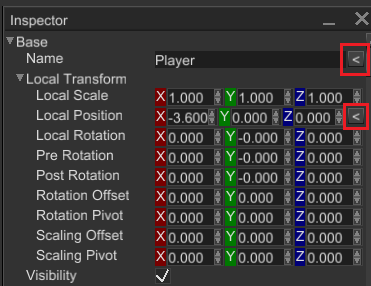
\includegraphics{images/scene_revert.png}
\caption{revert}
\end{figure}

Clicking on the \texttt{\textless{}} button will take the value from the parent prefab and the property won't be marked as modified anymore. In case there is no parent prefab, the button will just drop \texttt{modified} flag.

\section{Base node}\label{base-node}

Base node is a scene node that stores hierarchical information (a handle to the parent node and a set of handles to children nodes), local and global transform, name, tag, lifetime, etc. It has self-describing name - it is used as a base node for every other scene node (via composition).

It has no graphical information, so it is invisible all the time, but it is useful as a ``container'' for children nodes.

\subsection{How to create}\label{how-to-create-2}

Use the \texttt{PivotBuilder} to create an instance of the Pivot node (remember \texttt{Base} node itself is used only to build other node types):

\begin{Shaded}
\begin{Highlighting}[]
\NormalTok{\{\{\#include ../code/snippets/src/scene/base.rs:build\_node\}\}}
\end{Highlighting}
\end{Shaded}

\subsection{Building a complex hierarchy}\label{building-a-complex-hierarchy}

To build a complex hierarchy of some nodes, use \texttt{.with\_children()} method of the \texttt{BaseBuilder}, it allows you to build a hierarchy of any complexity:

\begin{Shaded}
\begin{Highlighting}[]
\NormalTok{\{\{\#include ../code/snippets/src/scene/base.rs:build\_complex\_node\}\}}
\end{Highlighting}
\end{Shaded}

Note that when we're building a \texttt{Camera} instance, we're passing a new instance of \texttt{BaseBuilder} to it, this instance can also be used to set some properties and a set of children nodes.

The ``fluent syntax'' is not mandatory to use, the above code snipped could be rewritten like this:

\begin{Shaded}
\begin{Highlighting}[]
\NormalTok{\{\{\#include ../code/snippets/src/scene/base.rs:build\_complex\_node\_flat\}\}}
\end{Highlighting}
\end{Shaded}

However, it looks less informative, because it loses the hierarchical view and it is harder to tell the relations between objects.

\subsection{Transform}\label{transform}

Base node has a local transform that allows you to translate/scale/rotate/etc. your node as you want to. For example, to move a node at specific location you could use this:

\begin{Shaded}
\begin{Highlighting}[]
\NormalTok{\{\{\#include ../code/snippets/src/scene/base.rs:translate\_node\}\}}
\end{Highlighting}
\end{Shaded}

You could also chain multiple \texttt{set\_x} calls, like so:

\begin{Shaded}
\begin{Highlighting}[]
\NormalTok{\{\{\#include ../code/snippets/src/scene/base.rs:transform\_node\}\}}
\end{Highlighting}
\end{Shaded}

See more info about transformations \href{./transform.md}{here}.

\subsection{Visibility}\label{visibility}

\texttt{Base} node stores all info about local visibility and global visibility (with parent's chain visibility included). Changing node's visibility could be useful if you want to improve performance by hiding distant objects (however it strongly advised to use level-of-detail for this) or to hide some objects in your scene. There are three main methods to set or fetch visibility:

\begin{itemize}
\tightlist
\item
  \texttt{set\_visibility} - sets local visibility for a node.
\item
  \texttt{visibility} - returns current local visibility of a node.
\item
  \texttt{global\_visibility} - returns combined visibility of a node. It includes visibility of every parent node in the hierarchy, so if you have a parent node with some children nodes and set parent's visibility to \texttt{false}, global visibility of children nodes will be \texttt{false} too, even if local visibility is \texttt{true}. This is useful technique for hiding complex objects with lots of children nodes.
\end{itemize}

\subsection{Enabling/disabling scene nodes}\label{enablingdisabling-scene-nodes}

A scene node could be enabled or disabled. Disabled nodes are excluded from a game loop and has almost zero CPU consumption (their global transform/visibility/enabled state is still updated due to limitations of the engine). Disabling a node could be useful if you need to completely freeze some hierarchy and do keep it in this state until it is enabled again. It could be useful to disable parts of a scene with which a player cannot interact to improve performance. Keep in mind, that enabled state is hierarchical like visibility. When you're disabling a parent node with some children nodes, the children nodes will be disabled too.

\section{Mesh node}\label{mesh-node}

Mesh is a scene node that represents a 3D model. This one of the most commonly used nodes in almost every game. Meshes could be easily created either programmatically or be made in some 3D modelling software (like Blender) and loaded in your scene.

\subsection{Surfaces}\label{surfaces}

Surface is a set of triangles that uses the same \href{../rendering/materials.md}{material}. Mesh node could contain zero of more surfaces; each surface contains a set of vertices and indices that binds vertices with triangles. Mesh nodes split into surfaces to be rendered effectively by modern GPUs.

\subsection{How to create}\label{how-to-create-3}

There are basically two ways, how to pick one depends on your needs. In general, using a 3D modelling software is the way to go, especially with tons and tons of free 3D models available online.

\begin{quote}
⚠️ The engine supports \emph{only} FBX and GLTF file format for 3D models! To use GLTF, specify \texttt{gltf} feature of the engine in your root Cargo.toml
\end{quote}

\subsubsection{Using a 3D modelling software}\label{using-a-3d-modelling-software}

To create a 3D model, you could use \href{https://www.blender.org/}{Blender} and then export it to \texttt{FBX} file format. To load your 3D model in the game, you should do few simple steps (loading a 3D model does not differ from a prefab instantiation):

\begin{Shaded}
\begin{Highlighting}[]
\NormalTok{\{\{\#include ../code/snippets/src/scene/mesh.rs:load\_model\_to\_scene\}\}}
\end{Highlighting}
\end{Shaded}

This code snippet intentionally omits proper \texttt{async/await} usage (instead it just blocks current thread until model is loading) and error handling. In the real game you should carefully handle all errors and use \texttt{async/await} properly.

\subsubsection{Creating a procedural mesh}\label{creating-a-procedural-mesh}

A mesh instance could be created from code, such meshes are called ``procedural''. They're suitable for cases when you cannot create a mesh in 3D modelling software.

\begin{Shaded}
\begin{Highlighting}[]
\NormalTok{\{\{\#include ../code/snippets/src/scene/mesh.rs:create\_procedural\_mesh\}\}}
\end{Highlighting}
\end{Shaded}

As you can see, creating a mesh procedurally requires lots of manual work and not so easy.

\subsection{Animation}\label{animation-1}

Mesh node supports bone-based animation (skinning) and blend shapes. See \href{./../animation/animation.md}{Animation chapter} for more info.

\subsection{Data Buffers}\label{data-buffers}

It is possible to access vertex buffer and index buffer of a mesh to either read or write some data there. For example, the following code extracts world-space positions of every vertex of an animated mesh:

\begin{Shaded}
\begin{Highlighting}[]
\NormalTok{\{\{\#include ../code/snippets/src/scene/mesh.rs:extract\_world\_space\_vertices\}\}}
\end{Highlighting}
\end{Shaded}

\section{Light node}\label{light-node}

The engine offers complex lighting system with various types of light sources.

\subsection{Light types}\label{light-types}

There are three main types of light sources: directional, point, and spotlights.

\subsubsection{Directional light}\label{directional-light}

Directional light does not have a position, its rays are always parallel, and it has a particular direction in space. An example of directional light in real-life could be our Sun. Even if it is a point light, it is so far away from the Earth, so we can assume that its rays are always parallel. Directional light sources are suitable for outdoor scenes.

A directional light source could be created like this:

\begin{Shaded}
\begin{Highlighting}[]
\NormalTok{\{\{\#include ../code/snippets/src/scene/light.rs:create\_directional\_light\}\}}
\end{Highlighting}
\end{Shaded}

By default, the light source will be oriented to lit ``the ground''. In other words its direction will be faced towards \texttt{(0.0,\ -1.0,\ 0.0)} vector. You can rotate it as you want by setting local transform of it while building. Something like this:

\begin{Shaded}
\begin{Highlighting}[]
\NormalTok{\{\{\#include ../code/snippets/src/scene/light.rs:create\_oriented\_directional\_light\}\}}
\end{Highlighting}
\end{Shaded}

\subsubsection{Point light}\label{point-light}

Point light is a light source that emits lights in all directions, it has a position, but does not have an orientation. An example of a point light source: light bulb.

\begin{Shaded}
\begin{Highlighting}[]
\NormalTok{\{\{\#include ../code/snippets/src/scene/light.rs:create\_point\_light\}\}}
\end{Highlighting}
\end{Shaded}

\subsubsection{Spotlight}\label{spotlight}

Spotlight is a light source that emits lights in cone shape, it has a position and orientation. An example of a spotlight source: flashlight.

\begin{Shaded}
\begin{Highlighting}[]
\NormalTok{\{\{\#include ../code/snippets/src/scene/light.rs:create\_spot\_light\}\}}
\end{Highlighting}
\end{Shaded}

\subsection{Light scattering}\label{light-scattering}

\begin{figure}
\centering
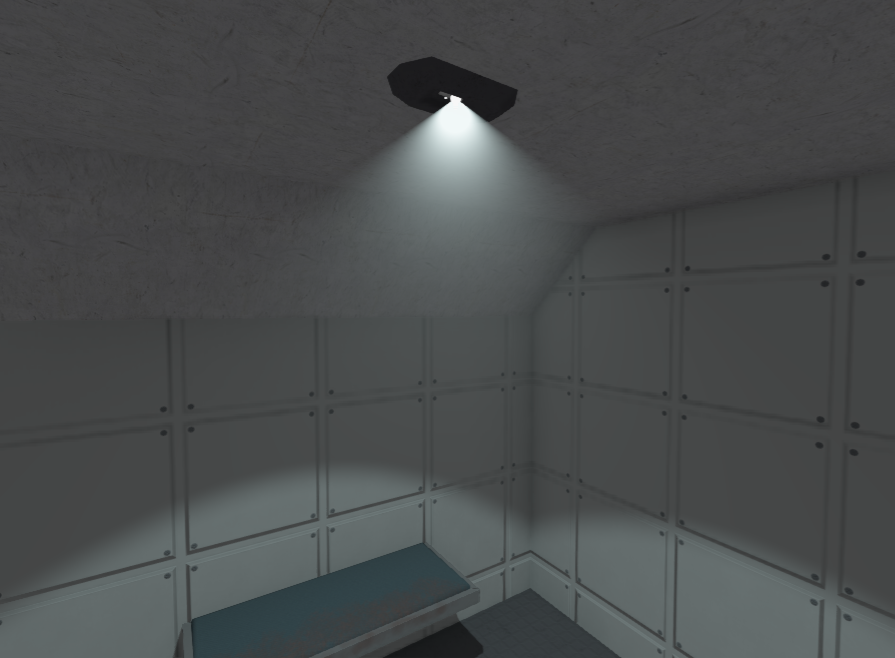
\includegraphics{images/scene_scattering.png}
\caption{scattering}
\end{figure}

Spot and point lights support light scattering effect. Imagine you're walking with a flashlight in a foggy weather, the fog will scatter the light from your flashlight making it, so you'll see the ``light volume''. Light scattering is \textbf{enabled by default}, so you don't have to do anything to enable it. However, in some cases you might want to disable it, you can do this either while building a light source or change light scattering options on existing light source. Here is the small example of how to do that.

\begin{Shaded}
\begin{Highlighting}[]
\NormalTok{\{\{\#include ../code/snippets/src/scene/light.rs:disable\_light\_scatter\}\}}
\end{Highlighting}
\end{Shaded}

You could also change the amount of scattering per each color channel, using this you could imitate the \href{https://en.wikipedia.org/wiki/Rayleigh_scattering}{Rayleigh scattering}:

\begin{Shaded}
\begin{Highlighting}[]
\NormalTok{\{\{\#include ../code/snippets/src/scene/light.rs:use\_rayleigh\_scattering\}\}}
\end{Highlighting}
\end{Shaded}

\subsection{Shadows}\label{shadows}

By default, light sources cast shadows. You can change this by using \texttt{set\_cast\_shadows} method of a light source. You should carefully manage shadows: shadows giving the most significant performance impact, you should keep the amount of light sources that can cast shadows at lowest possible amount to keep performance at good levels. You can also turn on/off shadows when you need:

\begin{Shaded}
\begin{Highlighting}[]
\NormalTok{\{\{\#include ../code/snippets/src/scene/light.rs:switch\_shadows\}\}}
\end{Highlighting}
\end{Shaded}

Not every light should cast shadows, for example a small light that a player can see only in a distance can have shadows disabled. You should set the appropriate values depending on your scene, just remember: the fewer the shadows the better the performance. The most expensive shadows are from point lights, the less, from spotlights and directional lights.

\subsection{Performance}\label{performance-2}

Lights are not cheap, every light source has some performance impact. As a general rule, try to keep the amount of light sources at reasonable levels and especially try to avoid creating tons of light sources in a small area. Keep in mind that the less area the light needs to ``cover'', the higher the performance. This means that you can have tons of small light sources for free.

\section{Sprite}\label{sprite}

Sprite is just a quad mesh that is always facing camera. It has size, color, rotation around ``look'' axis and a texture. Sprites are useful mostly for projectiles, like glowing plasma, and for things that should always face a camera.

\begin{quote}
⚠️ It should be noted that \textbf{sprites are not meant to be used for 2D games}, they're only for 3D. Use \href{./rectangle.md}{Rectangle node} if you need 2D sprites.
\end{quote}

\subsection{How to create}\label{how-to-create-4}

A sprite instance could be created using \texttt{SpriteBuilder}:

\begin{Shaded}
\begin{Highlighting}[]
\NormalTok{\{\{\#include ../code/snippets/src/scene/sprite.rs:create\_sprite\}\}}
\end{Highlighting}
\end{Shaded}

A sprite with a texture could be created by using \texttt{.with\_material} method of the builder:

\begin{Shaded}
\begin{Highlighting}[]
\NormalTok{\{\{\#include ../code/snippets/src/scene/sprite.rs:create\_sprite\_with\_texture\}\}}
\end{Highlighting}
\end{Shaded}

Please note, that this code create a material per each sprite. This could be very unoptimal if you're using tons of sprites at once, share the same material resource across multiple sprites if you can. Otherwise, each sprite will be rendered in a separate draw call and the overall performance will be very low.

\subsection{Animation}\label{animation-2}

See \href{../animation/spritesheet/spritesheet.md}{Sprite Animation} chapter for more info.

\subsection{General rules}\label{general-rules}

Sprites \textbf{must not} be used to create any visual effects that involve many particles. You should use \href{particle_system_node.md}{particle systems} for that. Why so? Particles systems are very well optimized for managing huge amounts of particles at the same time, but sprites are not. Each sprite is quite heavy to be used as a particle in particle systems, it has a lot of ``useless'' info that will eat a lot of memory.

\section{Particle system}\label{particle-system}

Particle system is a scene node that is used to create complex visual effects (VFX). It operates on huge amount of particles at once allowing you to do complex simulation that involves large amount of particles. Typically, particle systems are used to create following visual effects: smoke, sparks, blood splatters, steam, etc.

\begin{figure}
\centering
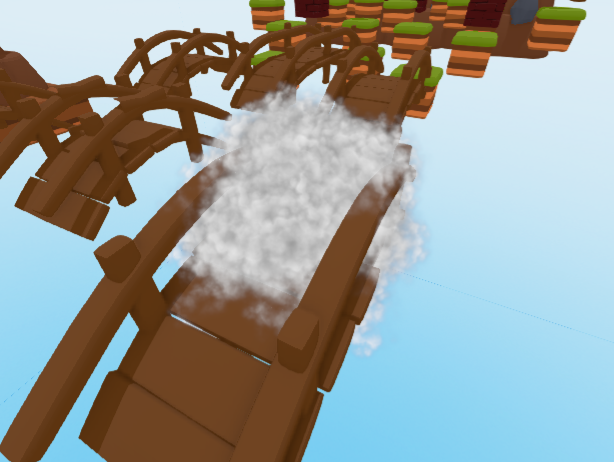
\includegraphics{images/scene_particle_system_example.png}
\caption{smoke}
\end{figure}

\subsection{Basic Concepts}\label{basic-concepts-1}

Particle system uses \emph{single} texture for every particle in the system, only Red channel is used. Red channel interpreted as an alpha for all particles.

Every particle is affected by \texttt{Acceleration} parameters of the particle system. It defines acceleration (in m/s2) that will affect velocities of every particle. It is used to simulate gravity.

\subsubsection{Particle}\label{particle}

Particle is a square (not quadrilateral, this is important) with a texture which is always facing towards camera. It has the following properties:

\begin{itemize}
\tightlist
\item
  \texttt{Position} - defines a position in \emph{local} coordinates of particle system (this means that if you rotate a particle system, all particles will be rotated too).
\item
  \texttt{Velocity} - defines a speed vector (in local coordinates) that will be used to modify local position of the particle each frame.
\item
  \texttt{Size} - size (in meters) of the square shape of the particle.
\item
  \texttt{Size\ Modifier} - a numeric value (in meters per second), that will be added to the Size at each frame, it is used to modify size of the particles.
\item
  \texttt{Lifetime} - amount of time (in seconds) that the particle can be active for.
\item
  \texttt{Rotation} - angle (in radians) that defines rotation around particle-to-camera axis (clockwise).
\item
  \texttt{Rotation\ Speed} - speed (in radians per second, rad/s) of rotation of the particle.
\item
  \texttt{Color} - RGBA color of the particle.
\end{itemize}

\subsubsection{Emitters}\label{emitters}

Particle system uses \emph{emitters} to define a set of zones where particles will be spawned, it also defines initial ranges of parameters of particles. Particle system must have at least one emitter to generate particles.

Emitter can be one of the following types:

\begin{itemize}
\tightlist
\item
  \texttt{Cuboid} - emits particles uniformly in a cuboid shape, the shape cannot be rotated, only translated.
\item
  \texttt{Sphere} - emits particles uniformly in a sphere shape.
\item
  \texttt{Cylinder} - emits particle uniformly in a cylinder shape, the shape cannot be rotated, only translated.
\end{itemize}

Each emitter have fixed set of parameters that affects \emph{initial} values for every spawned particle:

\begin{itemize}
\tightlist
\item
  \texttt{Position} - emitter have its own \emph{local} position (position relative to parent particle system node), this helps you to create complex particle systems that may spawn particles from multiple zones in space at once.
\item
  \texttt{Max\ Particles} - maximum amount of particles available for spawn. By default, it is \texttt{None}, which says that there is no limit.
\item
  \texttt{Spawn\ Rate} - rate (in units per second) defines how fast the emitter will spawn particles.
\item
  \texttt{Lifetime\ Range} - numeric range (in seconds) for particle lifetime values. The lower the beginning of the range the less spawned particles will live, and vice versa.
\item
  \texttt{Size\ Range} - numeric range (in meters) for particle size.
\item
  \texttt{Size\ Modifier\ Range} - numeric range (in meters per second, m/s) for particle size modifier parameter.
\item
  \texttt{X/Y/Z\ Velocity\ Range} - a numeric range (in meters per second, m/s) for a respective velocity axis (X, Y, Z) that defines initial speed along the axis.
\item
  \texttt{Rotation\ Range} - a numeric range (in radians) for initial rotation of a new particle.
\item
  \texttt{Rotation\ Speed\ Range} - a numeric range (in radians per second, rad/s) for rotation speed of a new particle.
\end{itemize}

\textbf{Important:} Every range (like Lifetime Range, Size Range, etc.) parameter generates \emph{random} value for respective parameter of a particle. You can tweak the seed of current random number generator (\texttt{fyrox::core::thread\_rng()}) to ensure that generated values will be different each time.

\subsection{How to create}\label{how-to-create-5}

There are multiple ways of creating a particle system, pick one that best suits your current needs.

\subsubsection{Using the editor}\label{using-the-editor}

The best way to create a particle system is to configure it in the editor, creating from code is possible too (see below), but way harder and may be not intuitive, because of the large amount of parameters. The editor allows you see the result and tweak it very fast. Create a particle system by \texttt{Create\ -\textgreater{}\ Particle\ System} and then you can start editing its properties. By default, new particle system has one Sphere particle emitter, you can add new emitters by clicking \texttt{+} button at the right of \texttt{Emitters} property in the Inspector (or remove by clicking \texttt{-}). Here's a simple example:

\begin{figure}
\centering
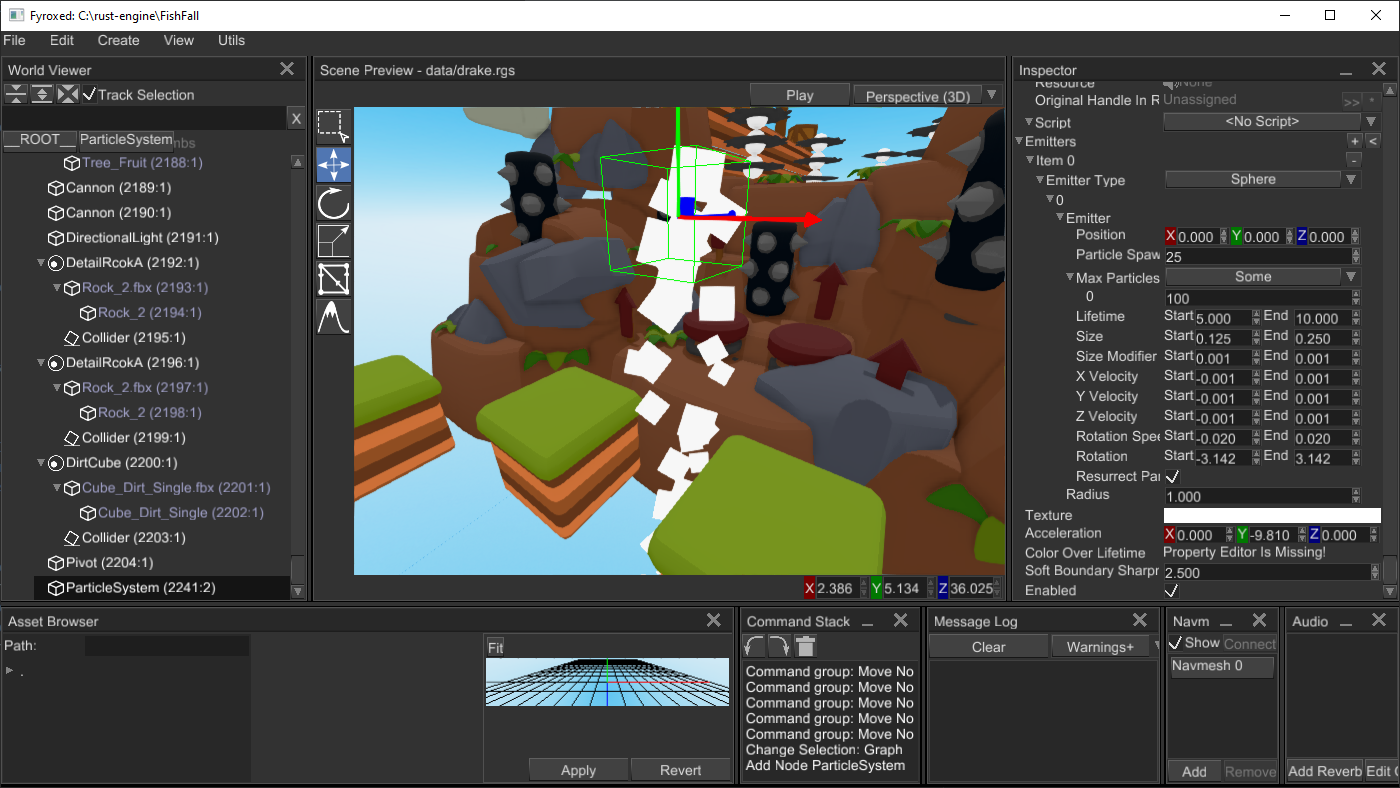
\includegraphics{images/scene_particle_system.png}
\caption{particle system}
\end{figure}

Now start tweaking desired parameters, it is hard to give any recommendations of how to achieve a particular effect, only practice matters here.

\subsubsection{Using the code}\label{using-the-code}

You can also create particle systems from code (in case if you need some procedurally-generated effects):

\begin{Shaded}
\begin{Highlighting}[]
\NormalTok{\{\{\#include ../code/snippets/src/scene/particle\_system.rs:create\_smoke\}\}}
\end{Highlighting}
\end{Shaded}

This code creates smoke effect with smooth dissolving (by using color-over-lifetime gradient). Please refer to \href{https://docs.rs/fyrox/latest/fyrox/scene/particle_system/index.html}{API docs} for particle system for more information.

\subsubsection{Using prefabs}\label{using-prefabs}

If you need to create particle systems made in the editor, you can always use prefabs. Create a scene with desired particle system and then \href{../resources/model.md\#instantiation}{instantiate} it to your scene.

\subsection{Soft particles}\label{soft-particles}

Fyrox used special technique, called soft particles, that smooths sharp transitions between particles and scene geometry:

\begin{figure}
\centering
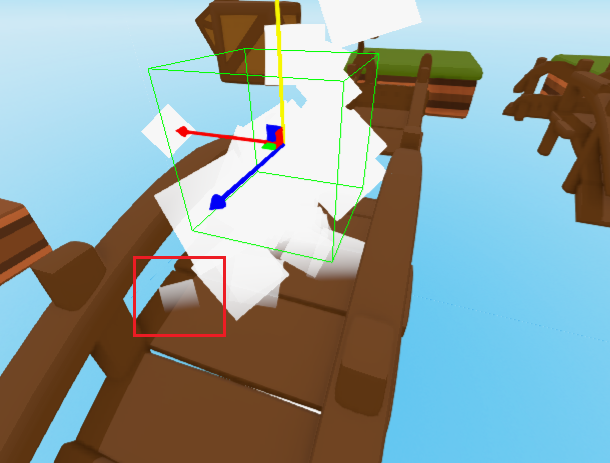
\includegraphics{images/scene_soft_particles.png}
\caption{soft particles}
\end{figure}

This technique especially useful for effects such as smoke, fog, etc. where you don't want to see the ``edge'' between particles and scene geometry. You can tweak this effect using \texttt{Soft\ Boundary\ Sharpness\ Factor}, the larger the value the more ``sharp'' the edge will be and vice versa.

\subsection{Restarting emission}\label{restarting-emission}

You can ``rewind'' particle systems in the ``initial'' state by calling \texttt{particle\_system.clear\_particles()} method, it will remove all generated particles and emission will start over.

\subsection{Enabling or disabling particle systems}\label{enabling-or-disabling-particle-systems}

By default, every particle system is enabled. Sometimes there is a need to create a particle system, but not enable it (for example for some delayed effect). You can achieve this by calling \texttt{particle\_system.set\_enabled(true/false)} method. Disabled particle systems will still be drawn, but emission and animation will be stopped. To hide particle system completely, use \texttt{particle\_system.set\_visibility(false)} method.

\subsection{Performance}\label{performance-3}

Particle systems using special renderer that optimized to draw millions of particles with very low overhead, however particles simulated on CPU side and may significantly impact overall performance when there are many particle systems with lots of particles in each.

\subsection{Limitations}\label{limitations}

Particle systems does not interact with lighting, this means that particles will not be lit by light sources in the scene.

\section{Terrain}\label{terrain}

Terrain is a scene node that represents uniform grid of cells where each cell can have different height. Other, commonly known name for terrain is heightmap. Terrains used to create maps for open-world games, it is used to create hills, mountains, plateau, roads, etc.

\begin{figure}
\centering
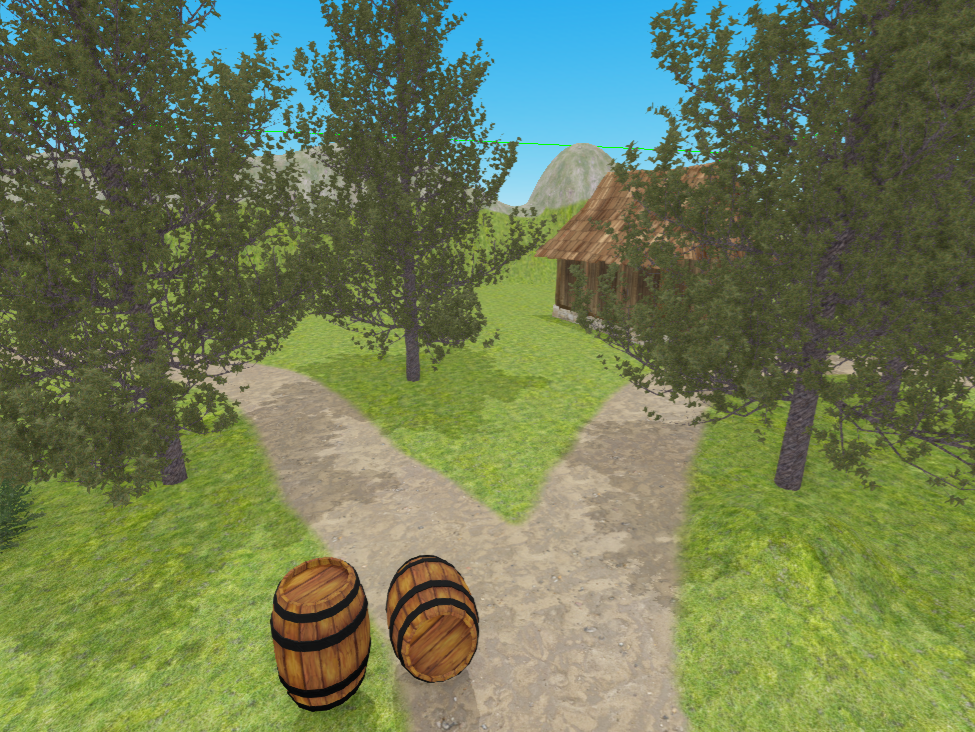
\includegraphics{images/scene_terrain.png}
\caption{terrain}
\end{figure}

\subsection{Basic concepts}\label{basic-concepts-2}

There are few basic concepts that you should understand before trying to use terrains. This will help you to understand design decisions and potential use cases.

\subsubsection{Heightmap}\label{heightmap}

As it was already mentioned, terrain is a uniform grid where X and Z coordinates of cells have fixed values, while Y can change. In this case we can store only width, height and resolution numerical parameters to calculate X and Z coordinates, while Y is stored in a separate array which is then used to modify heights of cells. Such array is called \emph{heightmap}.

\begin{figure}
\centering
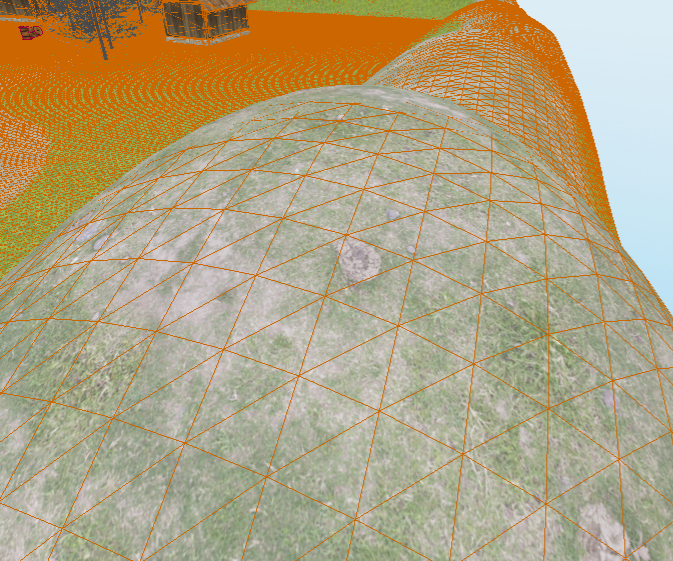
\includegraphics{images/scene_terrain_mesh.png}
\caption{terrain mesh}
\end{figure}

\subsubsection{Layers}\label{layers}

Layer is a material + mask applied to terrain's mesh. Mask is a separate, greyscale texture that defines in which parts of the terrain the material should be visible or not. White pixels in the mask makes the material to be visible, black - completely transparent, everything between helps you to create smooth transitions between layers. Here's a simple example of multiple layers:

\begin{figure}
\centering
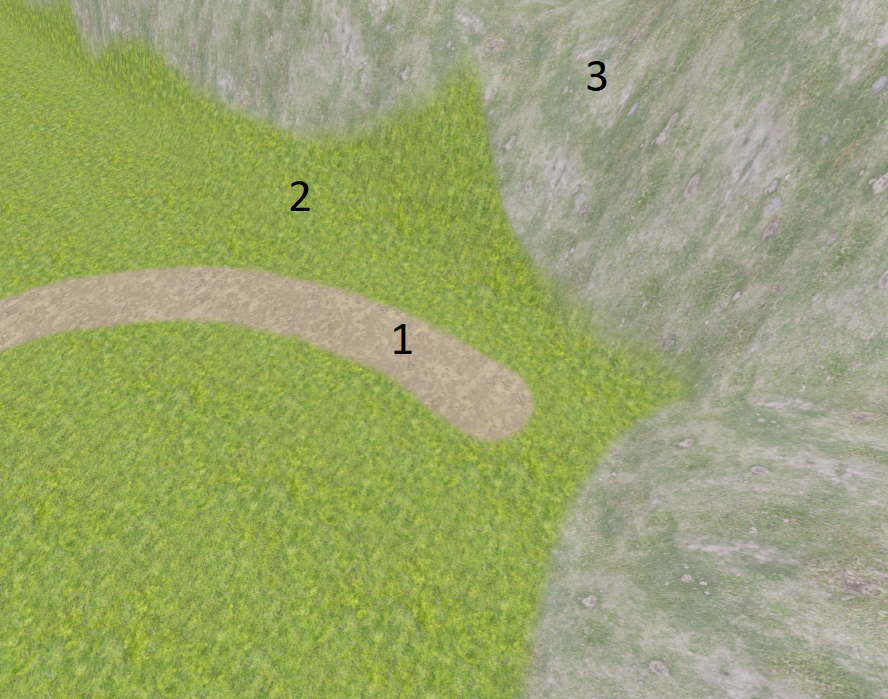
\includegraphics{images/scene_terrain_layers_layout.png}
\caption{terrain layers layout}
\end{figure}

There are 3 layers: 1 - dirt, 2 - grass, 3 - rocks and grass. As you can see, there are smooth transitions between each layer, it is achieved by layer's mask.

Each layer uses separate material, which can be edited from respective property editor in the Inspector:

\begin{figure}
\centering
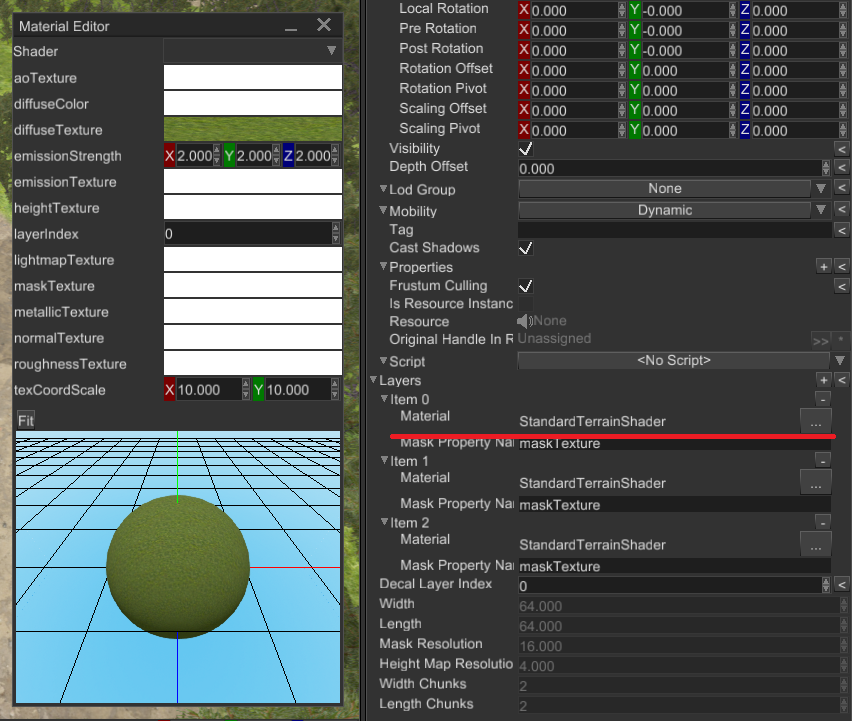
\includegraphics{images/scene_terrain_layer_material.png}
\caption{terrain layer material}
\end{figure}

\subsection{Creating terrain in the editor}\label{creating-terrain-in-the-editor}

You can create a terrain node by clicking \texttt{Create\ -\textgreater{}\ Terrain}. It will create a terrain with fixed width, height, and resolution (see \href{./terrain_node.md\#limitations-and-known-issues}{limitations}). Once the terrain is created, select it in the World Viewer and click on Hill icon on the toolbar. This will enable terrain editing, brush options panel should also appear. See the picture below with all the steps:

\begin{figure}
\centering
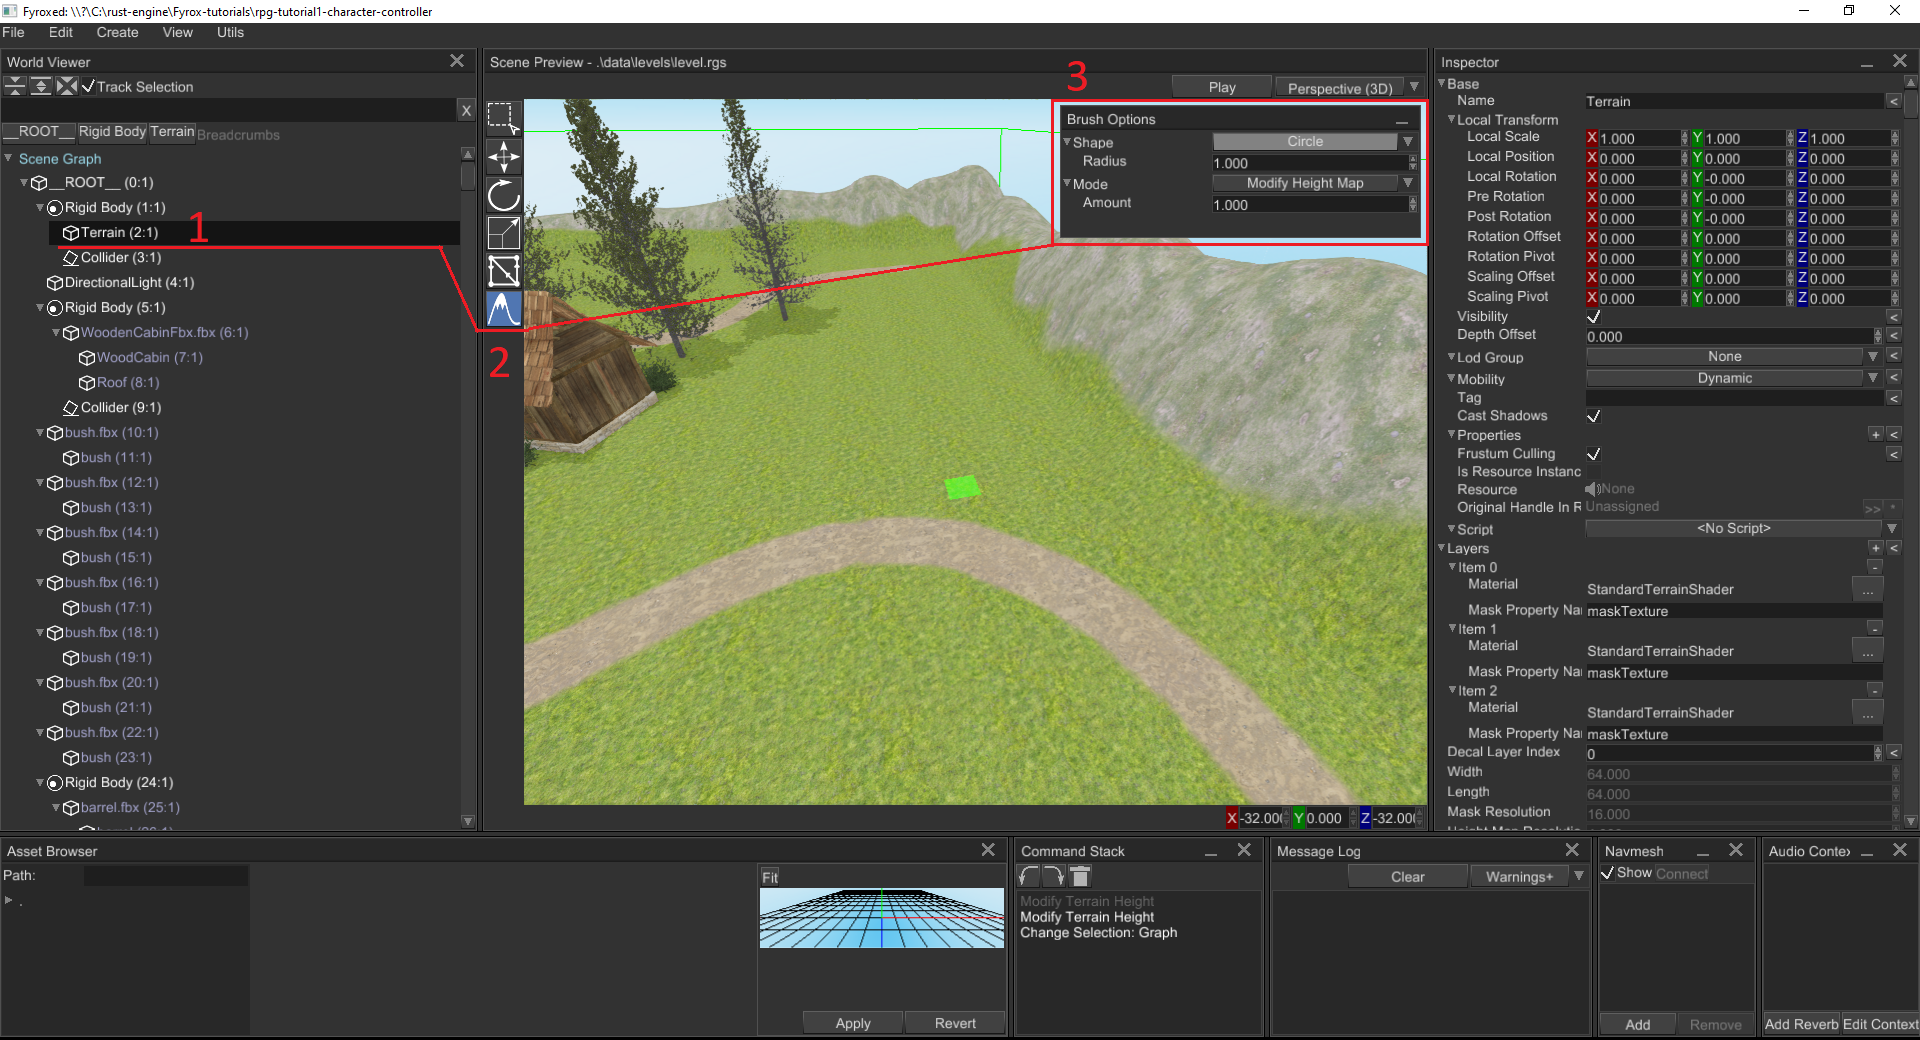
\includegraphics{images/scene_terrain_editing.png}
\caption{terrain editing}
\end{figure}

The green rectangle on the terrain under the cursor represents current brush. You can edit brush options in the \texttt{Brush\ Options} window:

\begin{figure}
\centering
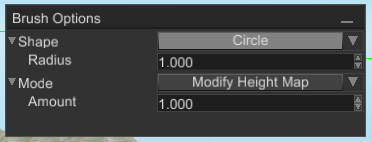
\includegraphics{images/scene_brush_options.png}
\caption{brush options}
\end{figure}

You can select a shape (either circle or rectangle with configurable size) and a mode (either modify the height map, or draw on mask of specific layer).

When editing terrain's height, left mouse button raises height map, but if \texttt{Shift} key is pressed it lowers it instead. Something similar is applied to the mask editing - left mouse button draws, but if hold \texttt{Shift} - it will erase mask content.

\subsection{Creating terrain from code}\label{creating-terrain-from-code}

Terrain can always be created from code, here's comprehensive example of how to create and modify terrain from code:

\begin{Shaded}
\begin{Highlighting}[]
\NormalTok{\{\{\#include ../code/snippets/src/scene/terrain.rs:create\_random\_two\_layer\_terrain\}\}}
\end{Highlighting}
\end{Shaded}

As you can see there is quite a lot of code, ideally you should use editor all the times, because handling everything from code could be very tedious. The result of its execution (if all textures are set correctly) could be something like this (keep in mind that terrain will be random every time you run the code):

\begin{figure}
\centering
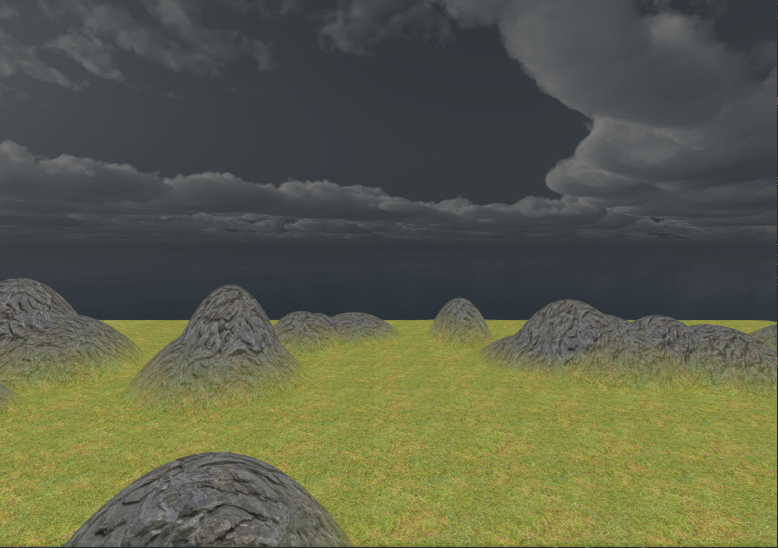
\includegraphics{images/scene_terrain_random.png}
\caption{terrain from code}
\end{figure}

\subsection{Physics}\label{physics-1}

By default, terrains does not have respective physical body and shape, it should be added manually. Create a static rigid body node with a collider with Heightmap shape (\href{../physics/collider.md}{learn more about colliders}). Then attach the terrain to the rigid body. Keep in mind that terrain's origin differs from Heightmap rigid body, so you need to offset the terrain to match its physical representation. Enable physics visualization in editor settings to see physical shapes and move terrain. Now to move the terrain you should move the body, instead of the terrain (because of parent-child \href{../beginning/scene_and_scene_graph.md\#local-and-global-coordinates}{relations}).

\subsection{Performance}\label{performance-4}

Terrain rendering complexity have linear dependency with the amount of layers terrain have. Each layer forces the engine to re-render terrain's geometry with different textures and mask. Typical amount of layers is from 4 to 8. For example, a terrain could have the following layers: dirt, grass, rock, snow. This is a relatively lightweight scheme. In any case, you should measure frame time to understand how each new layer affects performance in your case.

\subsection{Chunking}\label{chunking}

Terrain itself does not define any geometry or rendering data, instead it uses one or more chunks for that purpose. Each chunk could be considered as a ``sub-terrain''. You can ``stack'' any amount of chunks from any side of the terrain. To do that, you define a range of chunks along each axis. This is very useful if you need to extend your terrain in a particular direction. Imagine that you've created a terrain with just one chunk (\texttt{0..1} range on both axes), but suddenly you foundthat you need to extend the terrain to add some new game locations. In this case you can change the range of chunks at the desired axis. For instance, if you want to add a new location to the right from your single chunk, then you should change \texttt{width\_chunks} range to \texttt{0..2} and leave \texttt{length\_chunks} as is (\texttt{0..1}). This way terrain will be extended, and you can start shaping the new location.

\subsection{Level-of-detail}\label{level-of-detail}

Terrain has automatic LOD system, which means that the closest portions of it will be rendered with the highest possible quality (defined by the resolution of height map and masks), while the furthest portions will be rendered with the lowest quality. This effectively balances GPU load and allows you to render huge terrains with low overhead.

The main parameter that affects LOD system is \texttt{block\_size} (\texttt{Terrain::set\_block\_size}), which defines size of the patch that will be used for rendering. It is used to divide the size of the height map into a fixed set of blocks using quad-tree algorithm.

Current implementation uses modified version of CDLOD algorithm without patch morphing. Apparently it is not needed, since bilinear filtration in vertex shader prevents seams to occur.

Current implementation makes it possible to render huge terrains (64x64 km) with 4096x4096 heightmap resolution in about a millisecond on average low-to-middle-end GPU.

\subsection{Limitations and known issues}\label{limitations-and-known-issues}

There is no way to cut holes in the terrain yet, it makes impossible to create caves. There is also no way to create ledges, use separate meshes to imitate this. See \href{https://github.com/FyroxEngine/Fyrox/issues/351}{tracking issue} for more info.

\section{Camera node}\label{camera-node}

Camera is a special scene node that allows you to ``look'' at your scene from any point and with any orientation. Currently, the engine supports only \emph{perspective} cameras, which could be represented as a frustum volume. Everything that ``intersects'' with the frustum will be rendered.

\begin{figure}
\centering
\includesvg{images/scene_frustum.svg}
\caption{Frustum}
\end{figure}

\subsection{How to create}\label{how-to-create-6}

An instance of camera node could be created using \texttt{CameraBuilder}:

\begin{Shaded}
\begin{Highlighting}[]
\NormalTok{\{\{\#include ../code/snippets/src/scene/camera.rs:create\_camera\}\}}
\end{Highlighting}
\end{Shaded}

Orientation and position should be set in \texttt{BaseBuilder} as usual.

\subsection{Projection modes}\label{projection-modes}

Projection mode defines how your scene will look like after rendering, there are two projection modes available.

\subsubsection{Perspective}\label{perspective}

Perspective projection makes distant objects smaller and parallel lines converging when using it, it is the most common projection type for 3D games. By default, each camera uses perspective projection. It's defined by three parameters that describes frustum volume:

\begin{itemize}
\tightlist
\item
  Field of view angle
\item
  Near clipping plane location
\item
  Far clipping plane location
\end{itemize}

Here is a simple example of how to create a camera with perspective projection:

\begin{Shaded}
\begin{Highlighting}[]
\NormalTok{\{\{\#include ../code/snippets/src/scene/camera.rs:create\_perspective\_camera\}\}}
\end{Highlighting}
\end{Shaded}

\subsubsection{Orthographic}\label{orthographic}

Orthographic projection prevents parallel lines from converging, it does not affect object size with distance. If you're making 2D games or isometric 3D games, this is the projection mode you're looking for. Orthographic projection defined by three parameters:

\begin{itemize}
\tightlist
\item
  Vertical Size
\item
  Near Clipping Plane
\item
  Far Clipping Plane
\end{itemize}

Vertical size defines how large the ``box'' will be in vertical axis, horizontal size is derived from vertical size by multiplying vertical size with aspect ratio.

Here is a simple example of how to create a camera with orthographic projection:

\begin{Shaded}
\begin{Highlighting}[]

\end{Highlighting}
\end{Shaded}

\subsection{Performance}\label{performance-5}

Each camera forces engine to re-render scene one more time, which can be very resource-intensive (both CPU and GPU) operation.

To reduce GPU load, try to keep the Far Clipping Plane at lowest possible values. For example, if you're making a game with closed environment (lots of corridors, small rooms, etc.) set the Far clipping Plane to max possible distance that can be ``seen'' in your game - if the largest thing is a corridor, then set the Far clipping Plane to slightly exceed the length. This will force the engine to clip everything that is out of bounds and do not draw such objects.

\subsection{Skybox}\label{skybox}

Outdoor scenes usually have distant objects that can't be reached, these can be mountains, sky, distant forest, etc. such objects can be pre-rendered and then applied to a huge cube around camera, it will always be rendered first and will be the background of your scene. To create a Skybox and set it to a camera, you can use the following code:

\begin{Shaded}
\begin{Highlighting}[]
\NormalTok{\{\{\#include ../code/snippets/src/scene/camera.rs:create\_camera\_with\_skybox\}\}}
\end{Highlighting}
\end{Shaded}

\subsection{Color grading look-up tables}\label{color-grading-look-up-tables}

Color grading Look-Up Tables (LUT) allows you to transform color space of your frame. Probably everyone saw the famous ``mexican'' movie effect when everything becomes yellow-ish when action takes place in Mexico, this is done via color grading LUT effect. When used wisely, it can significantly improve perception of your scene.

Here is the same scene having no color correction along with another case that has ``mexico'' color correction:

\begin{longtable}[]{@{}
  >{\raggedright\arraybackslash}p{(\columnwidth - 2\tabcolsep) * \real{0.6111}}
  >{\raggedright\arraybackslash}p{(\columnwidth - 2\tabcolsep) * \real{0.3889}}@{}}
\toprule\noalign{}
\begin{minipage}[b]{\linewidth}\raggedright
Scene
\end{minipage} & \begin{minipage}[b]{\linewidth}\raggedright
Look-up-table
\end{minipage} \\
\midrule\noalign{}
\endhead
\bottomrule\noalign{}
\endlastfoot
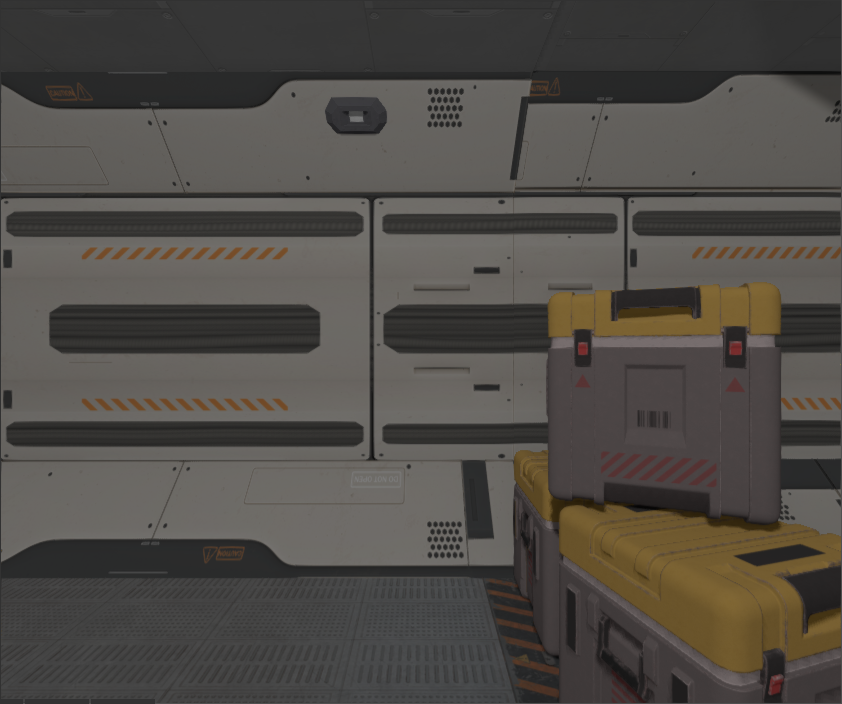
\includegraphics{images/scene_no_color_correction.PNG} & 
\includegraphics{images/scene_lut_neutral.jpg} \\
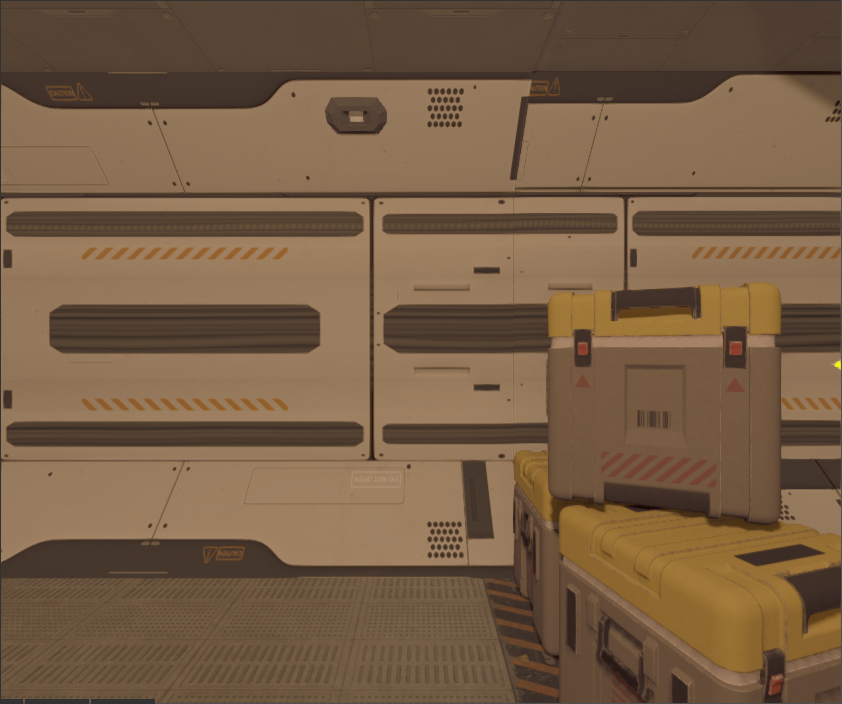
\includegraphics{images/scene_with_color_correction.PNG} & 
\includegraphics{images/scene_lut_mexico.jpg} \\
\end{longtable}

To use color grading LUT you could do something like this:

\begin{Shaded}
\begin{Highlighting}[]
\NormalTok{\{\{\#include ../code/snippets/src/scene/camera.rs:create\_camera\_with\_lut\}\}}
\end{Highlighting}
\end{Shaded}

\subsection{Picking}\label{picking}

In some games you may need to do mouse picking of objects in your scene. To do that, at first you need to somehow convert a point on the screen to ray in the world. \texttt{Camera} has \texttt{make\_ray} method exactly for that purpose:

\begin{Shaded}
\begin{Highlighting}[]
\NormalTok{\{\{\#include ../code/snippets/src/scene/camera.rs:make\_picking\_ray\}\}}
\end{Highlighting}
\end{Shaded}

The ray then can be used to \href{../physics/ray.md}{perform a ray cast over physics entities}. This is the simplest way of camera picking, and you should prefer it most of the time.

\subsubsection{Advanced picking}\label{advanced-picking}

\textbf{Important}: The following picking method is for advanced engine users only, if you don't know the math you should not use it.

If you know the math and don't want to create physical entities, you can use this ray to perform manual ray intersection check:

\begin{Shaded}
\begin{Highlighting}[]
\NormalTok{\{\{\#include ../code/snippets/src/scene/camera.rs:precise\_ray\_test\}\}}
\end{Highlighting}
\end{Shaded}

\texttt{precise\_ray\_test} is what you need, it performs precise intersection check with geometry of a mesh node. It returns a tuple of the closest distance and the closest intersection point.

\section{Exposure and HDR}\label{exposure-and-hdr}

(WIP)

\section{Decal node}\label{decal-node}

Decal nodes allow you to ``project'' a texture onto your scene within some specific bounds. It is widely used for bullet holes, blood splatter, dirt, cracks and so on. Here is the example of the decal applied to the scene:

\begin{figure}
\centering
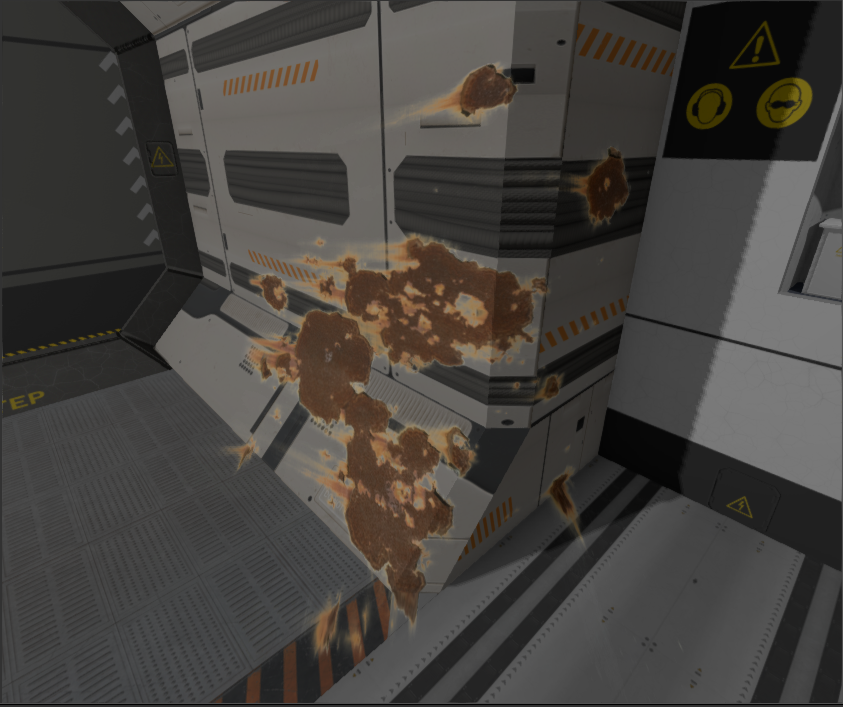
\includegraphics{images/scene_decal.PNG}
\caption{Decal}
\end{figure}

The rust marks are applied on existing geometry of the scene by projecting a rust texture in specific direction.

\subsection{How to create}\label{how-to-create-7}

A decal instance can be created using DecalBuilder:

\begin{Shaded}
\begin{Highlighting}[]
\NormalTok{\{\{\#include ../code/snippets/src/scene/decal.rs:create\_decal\}\}}
\end{Highlighting}
\end{Shaded}

\subsection{Textures}\label{textures}

You can specify which textures the decal will be projecting, currently there is only diffuse and normal maps supported.

\subsection{Rendering}\label{rendering-1}

Currently, the engine supports only \emph{deferred decals}, which means that decals modify the information stored in G-Buffer. This fact means that decals will be lit correctly with other geometry in the scene. However, if you have some objects in your scene that uses forward rendering path, your decals won't be applied to them.

\subsection{Bounds}\label{bounds}

Decal uses Object-Oriented Bounding Box (OOB) to determine pixels on which decal's textures will be projected, everything that got into OOB will be covered. Exact bounds can be set by tweaking local transform of a decal. If you want your decal to be larger, set its scale to some large value. To position a decal - use local position, to rotate - local rotation.

A decal defines a cube that projects a texture on every pixel of a scene that got into the cube. Exact cube size is defined by decal's local scale. For example, if you have a decal with scale of (1.0, 2.0, 0.1) then the size of the cube (in local coordinates) will be width = 1.0, height = 2.0 and depth = 0.1. The decal can be rotated as any other scene node. Its final size and orientation are defined by the chain of transformations of parent nodes.

\subsection{Layers}\label{layers-1}

There are situations when you want to prevent some geometry from being covered with a decal, to do that the engine offers a concept of layers. A decal will be applied to a geometry if and only if they have matching layer index. This allows you to create environment damage decals, and they won't affect dynamic objects since they're located on different layers.

\subsection{Performance}\label{performance-6}

Current implementation of decals is relatively cheap, this allows you to create many decals on scene. However, you should keep the amount of decals at a reasonable level.

\section{Rectangle node}\label{rectangle-node}

Rectangle is the simplest ``2D'' node, it can be used to create ``2D'' graphics. 2D is in quotes here because the node is actually a 3D node, like everything else in the engine. Here is an example scene made with the rectangle nodes and an orthographic camera:

\begin{figure}
\centering
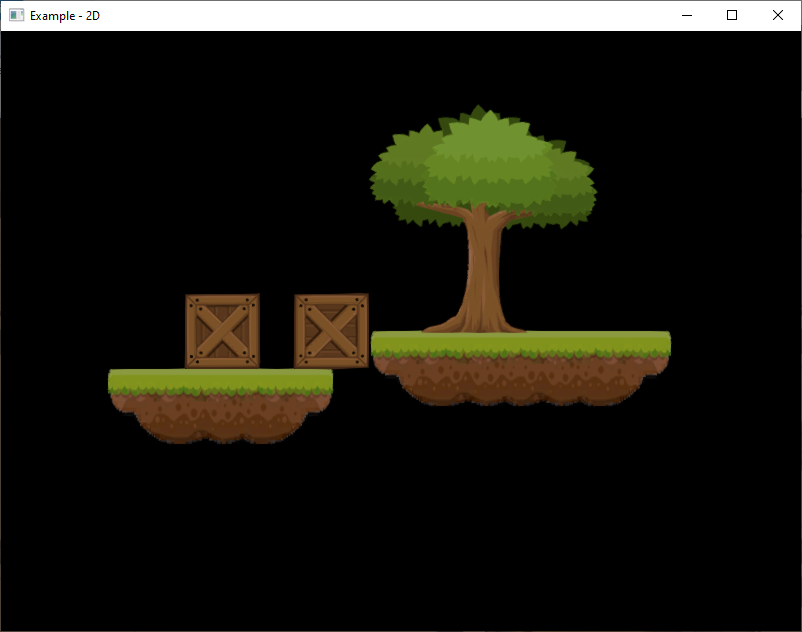
\includegraphics{images/scene_2d_scene.PNG}
\caption{2d scene}
\end{figure}

As you can see it is a good basis for 2D games.

\subsection{How to create}\label{how-to-create-8}

Use the RectangleBuilder to create Rectangle nodes:

\begin{Shaded}
\begin{Highlighting}[]
\NormalTok{\{\{\#include ../code/snippets/src/scene/rectangle.rs:create\_rect\}\}}
\end{Highlighting}
\end{Shaded}

\subsection{Specifying image portion for rendering}\label{specifying-image-portion-for-rendering}

By default, Rectangle node uses entire image for rendering, but for some applications it is not enough. For example, you may want to use sprite sheets to animate your 2D entities. In this case you need to be able to use only portion of an image. It is possible to do by using \texttt{set\_uv\_rect} method of the Rectangle node. Here's an example of setting right-top quarter of an image to be used by a Rectangle node:

\begin{Shaded}
\begin{Highlighting}[]
\NormalTok{\{\{\#include ../code/snippets/src/scene/rectangle.rs:set\_2nd\_quarter\_image\_portion\}\}}
\end{Highlighting}
\end{Shaded}

Keep in mind that every part of uv rectangle is proportional. For example 0.5 means 50\%, 1.5 = 150\% and so on. If width or height is exceeding 1.0 and the texture being used is set to Wrapping mode at respective axis, the image will tile across axes.

\subsection{Animation}\label{animation-3}

See \href{../animation/spritesheet/spritesheet.md}{Sprite Animation} chapter for more info.

\subsection{Performance}\label{performance-7}

Rectangles use specialized renderer that is heavily optimized to render tons of rectangles at once, so you can use rectangles almost for everything in 2D games.

\section{Custom Scene Node}\label{custom-scene-node}

Sometimes there is a need to have custom scene nodes, it is possible to do, but it requires quite a lot of boilerplate code.

\begin{Shaded}
\begin{Highlighting}[]
\NormalTok{\{\{\#include ../code/snippets/src/scene/custom.rs:custom\_node\}\}}
\end{Highlighting}
\end{Shaded}

Once the node is defined, you can create is as usual and put in the graph:

\begin{Shaded}
\begin{Highlighting}[]
\NormalTok{\{\{\#include ../code/snippets/src/scene/custom.rs:add\_custom\_node\}\}}
\end{Highlighting}
\end{Shaded}

\subsection{Limitations}\label{limitations-1}

Scene nodes have no access to outer context, this means that you cannot reference any data that is located outside graph easily. You still can define a global variable that \textbf{will} be accessible, but it is considered as a hack and should be avoided. If you want to add custom logic to scene nodes, then you should use scripts instead. Custom nodes are intended for very specific use cases, such as adding ``data sources'' for renderer, etc.

\subsection{Editor support}\label{editor-support}

For now, you cannot create custom nodes from the editor. This will be available in future versions of the engine.

\chapter{Physics}\label{physics-2}

The engine have full-featured physics engine under the hood (Rapier), it helps you to simulate physics in your games.
There is first-class support for both 2D and 3D physics. There are three main physics entities in the engine:

\begin{itemize}
\tightlist
\item
  Rigid Body - responsible for rigid body dynamics simulation, must have at least one collider to be able to interact with other rigid bodies in the world.
\item
  Collider - responsible for collision detection.
\item
  Joint - responsible for motion restriction between two rigid bodies.
\end{itemize}

All these entities are ordinary scene nodes, so they can be arranged into any hierarchy in the scene. However there some rules that have to be followed to make physics simulation work as intended:

\begin{itemize}
\tightlist
\item
  Rigid body node must have at least one \emph{direct child} Collider node, otherwise rigid body won't interact with other rigid bodies in the world.
\item
  Joint node must have two \emph{direct child} rigid bodies, otherwise joint will have no effect.
\end{itemize}

\subsection{Differences between 3D and 2D}\label{differences-between-3d-and-2d}

There is a very few differences between 3D and 2D physics, the most obvious is that 2D physics does simulation only in oXY plane (the plane of the screen). 2D physics has less collider shapes available since some 3D shapes degenerate in 2D, for example cylinder 3D shape in 2D is just a rectangle. There is also lesser amount of joints available in 2D, there is no revolute joint for example. Unlike 3D physics entities, 2D physics entities exist in the separate \texttt{scene::dim2} module.

\section{Rigid body node}\label{rigid-body-node}

Rigid body node is the one of main physical entities in the engine. Rigid body nodes can be affected by gravity, external forces and other rigid bodies. Use rigid body node everywhere you need natural physical behavior for your objects.

\subsection{How to create}\label{how-to-create-9}

Use RigidBodyBuilder to create a rigid body instance:

\begin{Shaded}
\begin{Highlighting}[]
\NormalTok{\{\{\#include ../code/snippets/src/scene/rigid\_body.rs:create\_cube\_rigid\_body\}\}}
\end{Highlighting}
\end{Shaded}

\subsection{Colliders}\label{colliders}

Rigid body must have at least one collider to participate in simulation properly, multiple colliders can be used to create complex shapes from simple shapes, you can create concave objects this way. Every collider \textbf{must} be a direct child node of a rigid body. In the editor it could look like this:

\begin{figure}
\centering
\includegraphics{./colliders.png}
\caption{colliders}
\end{figure}

Note that, \texttt{Box} node here is an instance of \texttt{Rigid\ Body\ 2D}, and it has \texttt{Collider\ 2D} as a child and some sprite. This structure (when a rigid body has a collider as a child) is mandatory for physics engine to work correctly! Collider won't work (participate in physical simulation) without a rigid body and a rigid body won't work without a collider. This applied to both 2D and 3D.

Keep in mind, that your graphical representation of an object (some node like \texttt{Mesh}, \texttt{Sprite}, etc.) must be attached to a rigid body. Otherwise, the rigid body will move, but the graphical representation won't. You can also arrange it other way around: a graphical node can have rigid body with a collider, but that requires the rigid body to be kinematic. This is used to create \href{./collider.md\#using-colliders-for-hit-boxes}{hit boxes}, or any other things that should have physical representation, but move together with graphical node.

\subsection{Force and torque}\label{force-and-torque}

You can apply forces and torque to any rigid body, but only dynamic bodies will be affected. There is two ways of applying force to a rigid body: at center of mass or at particular point at the body:

\begin{Shaded}
\begin{Highlighting}[]
\NormalTok{\{\{\#include ../code/snippets/src/scene/rigid\_body.rs:apply\_force\_and\_torque\}\}}
\end{Highlighting}
\end{Shaded}

\subsection{Kinematic rigid bodies}\label{kinematic-rigid-bodies}

Sometimes you may want to have direct control over position/rotation of a rigid body and tell the physics engine to not do simulation for the body. This can be achieved by making the rigid body \emph{kinematic}:

\begin{Shaded}
\begin{Highlighting}[]
\NormalTok{\{\{\#include ../code/snippets/src/scene/rigid\_body.rs:create\_kinematic\_rigid\_body\}\}}
\end{Highlighting}
\end{Shaded}

\subsection{Continuous collision detection}\label{continuous-collision-detection}

Fast-moving rigid bodies can ``fly through'' other objects (for example a bullet can completely ignore walls if it is moving too fast), this happens because of discrete calculation. This can be fixed by using continuous collision detection, to enable it use either \texttt{.with\_ccd\_enabled(state)} of \texttt{RigidBodyBuilder} or \texttt{.set\_ccd\_enabled(state)} of \texttt{RigidBody}.

\subsection{Dominance}\label{dominance}

Dominance allows you to set a priority of forces applied to rigid bodies. It defines which rigid body can affect what rigid body, for example you can set the highest dominance for actors and leave dominance of everything else at zero, this way actors will be able to push any other dynamic bodies, but dynamic bodies won't affect actors. This is useful when you don't want your actors be pushed by surrounding objects (like if someone throws a box at an actor, it will stay still if it has higher dominance)

\subsection{2D rigid bodies}\label{d-rigid-bodies}

2D rigid bodies have no difference with 3D, except the simulation happens in oXY plane and Z coordinate is ignored.

\section{Collider node}\label{collider-node}

Collider is a geometrical shape that is used for collision detection, contact manifold generation, etc. Colliders are used in pair with rigid bodies, they make rigid body participate in collisions.

\textbf{Important:} Colliders only works in pair with rigid bodies! Colliders won't be used by the engine, unless they are direct children of a rigid body. Read \href{./rigid_body.md\#colliders}{this chapter} for more info.

\subsection{Shapes}\label{shapes}

Collider can have almost any shape, the engine offers the following shapes for 3D:

\begin{itemize}
\tightlist
\item
  Ball - dynamic sphere shape.
\item
  Cylinder - dynamic cylinder shape.
\item
  Cone - dynamic cone shape.
\item
  Cuboid - dynamic box shape.
\item
  Capsule - dynamic capsule shape.
\item
  Segment - dynamic segment (``line'') shape
\item
  Triangle - simple dynamic triangle shape
\item
  Triangle mesh - static concave shape, can be used together with any static level geometry (wall, floors, ceilings,
  anything else)
\item
  Height field - static height field shape, can be used together with terrains.
\item
  Polyhedron - dynamic concave shape.
\end{itemize}

Also, there is a similar, but smaller set for 2D (because some shapes degenerate in 2D):

\begin{itemize}
\tightlist
\item
  Ball - dynamic circle shape.
\item
  Cuboid - dynamic rectangle shape.
\item
  Capsule - dynamic capsule shape.
\item
  Segment - dynamic segment (``line'') shape.
\item
  Triangle - dynamic triangle shape.
\item
  Trimesh - static triangle mesh shape.
\item
  Heightfield - static height field shape.
\end{itemize}

\emph{Dynamic} in both lists means that such shapes can be used together with \emph{dynamic} rigid bodies, they'll correctly handle
all collisions and simulation will look as it should. \emph{Static} means that such shape should be used only with \emph{static} rigid bodies.

\subsection{How to create}\label{how-to-create-10}

Use ColliderBuilder to create an instance of collider from code with any shape you want.

\begin{Shaded}
\begin{Highlighting}[]
\NormalTok{\{\{\#include ../code/snippets/src/scene/collider.rs:create\_capsule\_collider\}\}}
\end{Highlighting}
\end{Shaded}

In the editor you can use \texttt{MainMenu\ -\textgreater{}\ Create\ -\textgreater{}\ Physics\ -\textgreater{}\ Collider}, or right-click on a node in \texttt{World\ Viewer} and select \texttt{Add\ Child\ -\textgreater{}\ Physics\ -\textgreater{}\ Collider}. Collider must be direct child of a rigid body, colliders do nothing on their own!

\subsection{Collision filtering}\label{collision-filtering}

Sometimes there's a need to prevent collision between various groups of colliders. Fyrox supports bit-wise collision filtering exactly for this purpose. For instance, you may have two groups of colliders: actors and powerups, and you want the actors to completely ignore collisions with powerups (and vice versa). In this case you can set collision groups for actors like so:

\begin{figure}
\centering
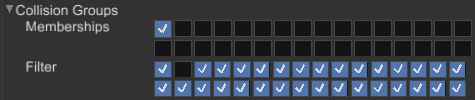
\includegraphics{images/physics_collision_groups_a.png}
\caption{actors collision groups}
\end{figure}

And set the collision groups for powerups like so:

\begin{figure}
\centering
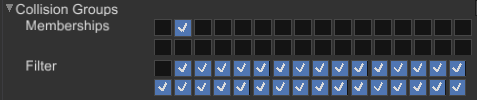
\includegraphics{images/physics_collision_groups_b.png}
\caption{powerups collision groups}
\end{figure}

As you can see, actors and powerups now have separate \texttt{memberships} (read - groups) and filters. This way, the actors will collide with everything, but powerups and vice versa.

\subsection{Using colliders for hit boxes}\label{using-colliders-for-hit-boxes}

You can use colliders to simulate hit boxes for your game characters. It can be done by creating a rigid body with \texttt{KinematicPositionBased} type and an appropriate collider as a child node. As the last step you need to attach the body to a bone in your character's model. Here's a quick example from the editor:

\begin{figure}
\centering
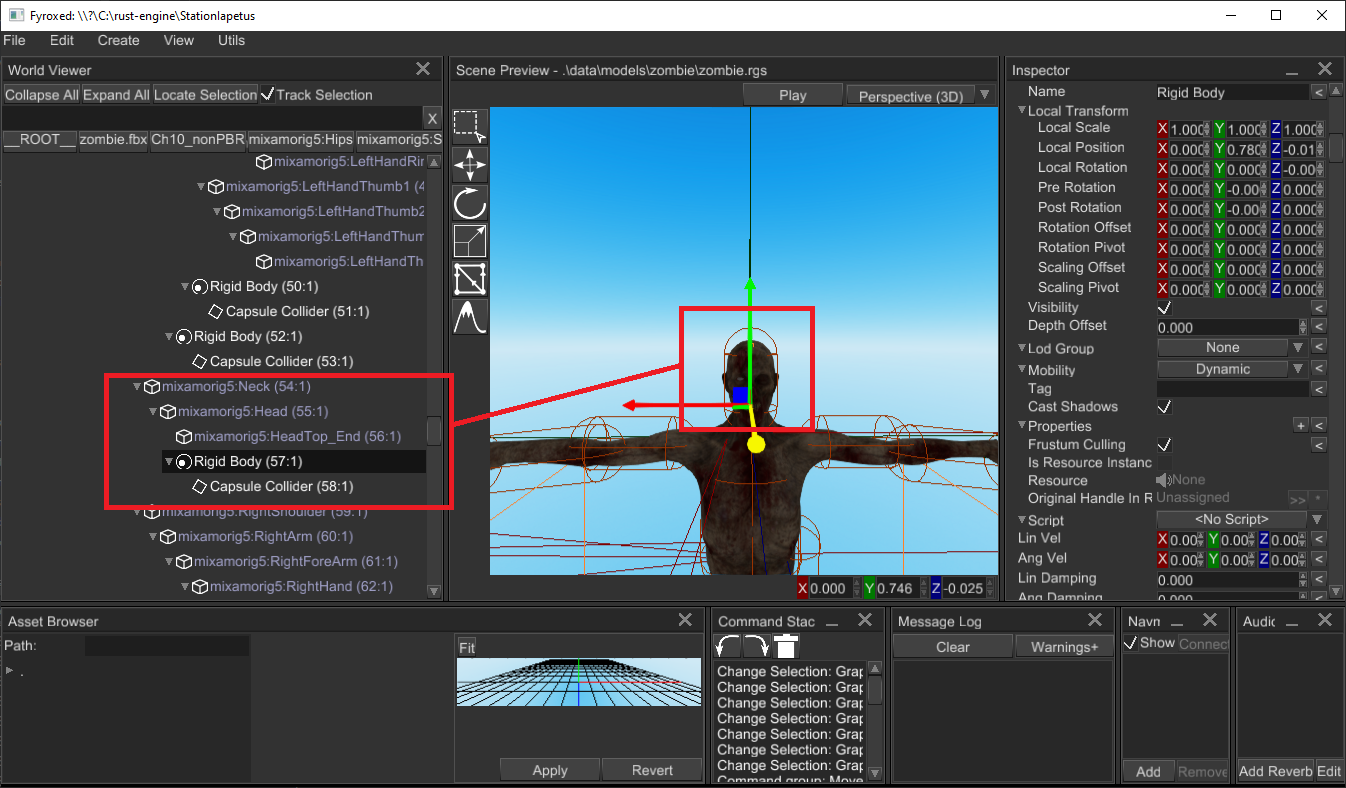
\includegraphics{images/physics_hitbox.png}
\caption{hitbox}
\end{figure}

As you can see, the rigid body has a capsule collider as a child and the body is attached to the neck bone. The body has \texttt{KinematicPositionBased} type, which will ensure that the body won't be simulated, instead its position will be synchronized with the position of the parent bone.

To actually use the hit boxes in your game, you can either use a ray-casting to perform a hit scan or you can use contacts information to fetch the stuff with which a hit box was contacted. See \href{./ray.md}{Ray casting} chapter of the section.

\section{Joint}\label{joint}

Joint is a configurable link between two rigid bodies, it restricts relative motion of two bodies. Fyrox provides a fixed set of joints that are suitable for various applications.

\begin{itemize}
\tightlist
\item
  Fixed Joint - hard link between two bodies, it is the same is if two rigid bodies were ``welded'' to each other with a metal rod.
\item
  Revolute Joint - restricts all translational movement and any rotations around Y and Z axes, but leaves rotation around local X axis free. An example of the joint from real world is a door hinge, it allows the door to rotate around single axis, but not move.
\item
  Prismatic Joint - restricts all rotations, movement is allowed along single axis (local X of the joint). An example of the joint from real world could be a slider that supports drawers on a table.
\item
  Ball Joint - restricts all movement, but leaves rotations unrestricted. An example of a ball joint from real world could be human shoulder.
\end{itemize}

2D joints does not have revolute joints, because it degenerates into ball joint.

\subsection{Bodies Binding}\label{bodies-binding}

When the joint is created and all bodies are set to it, it uses self global transform and bodies global transforms to calculate local frames for bodies. This process is called \emph{binding}, it happens once when the joint is created, but can be initiated by moving the joint to some other position by changing local transform of the joint.

\subsection{How to create}\label{how-to-create-11}

To create a joint from code use \texttt{JointBuilder}:

\begin{Shaded}
\begin{Highlighting}[]
\NormalTok{\{\{\#include ../code/snippets/src/scene/joint.rs:create\_joint\}\}}
\end{Highlighting}
\end{Shaded}

Once the joint is created, it will bind given bodies, using the process describe in the above section.

To create a joint from editor, use \texttt{MainMenu\ -\textgreater{}\ Create\ -\textgreater{}\ Physics\ -\textgreater{}\ Joint}, select the new joint and find \texttt{Body1} and \texttt{Body2} properties. Assign the fields by holding \texttt{Alt} key and drag'n'drop a rigid body to a field. Move the joint to correct position to ensure the binding will happen as intended.

\subsection{Limits}\label{limits}

You can restrict motion on primary joint axis (rotational and translational) by setting a limit to desired axis.

\begin{itemize}
\tightlist
\item
  Ball Joint have three angular limits, one per rotation around an axis. The angle range is given in radians.
\item
  Prismatic Joint have only one limit it is maximum linear distance between two bodies along primary joint axis.
\item
  Revolute Joint have a single angular limit around primary axis. The angle range is given in radians.
\item
  Fixed Joint does not have any limit setting, because it locks all degrees of freedom.
\end{itemize}

\subsection{Usage}\label{usage-2}

Joints can be used to create many game entities, such as doors, chains and rag dolls. The most interesting here is rag doll. It is used to create realistic behaviour for humans and creatures in games. In general, it is a set of rigid bodies, colliders and joints. Where each joint configured to match joints of a creature, for example ball joint could be used for shoulders, revolute joints for knees and elbows.

\section{Ray Casting}\label{ray-casting}

Ray casting allows you to query intersections of a ray with rigid bodies in a scene. Typical usage for ray casting is hit-scan weapons (weapons that shoots high-speed projectiles), AI collision avoidance, etc. To query intersections, use physics world instance of a scene graph:

\begin{Shaded}
\begin{Highlighting}[]
\NormalTok{\{\{\#include ../code/snippets/src/scene/ray.rs:do\_ray\_cast\}\}}
\end{Highlighting}
\end{Shaded}

The function above will return a collection of intersections that are sorted by intersection distance (a distance from beginning of the ray to an intersection point). Each intersection is represented by the following structure:

\begin{Shaded}
\begin{Highlighting}[]
\NormalTok{pub struct Intersection \{}
\NormalTok{    pub collider: Handle\textless{}Node\textgreater{},}
\NormalTok{    pub normal: Vector3\textless{}f32\textgreater{},}
\NormalTok{    pub position: Point3\textless{}f32\textgreater{},}
\NormalTok{    pub feature: FeatureId,}
\NormalTok{    pub toi: f32,}
\NormalTok{\}}
\end{Highlighting}
\end{Shaded}

\begin{itemize}
\tightlist
\item
  \texttt{collider} - a handle of the collider with which intersection was detected. To obtain a handle to rigid body, borrow the \texttt{collider} and fetch its \texttt{parent} field: \texttt{graph{[}collider{]}.parent()}.
\item
  \texttt{normal} - a normal at the intersection position in world coordinates.
\item
  \texttt{position} - a position of the intersection in world coordinates.
\item
  \texttt{feature} - additional data that contains a kind of the feature with which intersection was detected as well as its index. FeatureId::Face might have index that is greater than amount of triangles in a triangle mesh, this means that intersection was detected from ``back'' side of a face. To ``fix'' that index, simply subtract amount of triangles of a triangle mesh from the value.
\item
  \texttt{toi} - (\texttt{time\ of\ impact}) a distance from ray's origin to \texttt{position}.
\end{itemize}

\subsection{Avoiding unnecessary allocations}\label{avoiding-unnecessary-allocations}

As you might've noticed, the function above return \texttt{Vec\textless{}Intersection\textgreater{}} which allocates intersections on heap. This is relatively slow and could be sped up a lot by using static array on stack:

\begin{Shaded}
\begin{Highlighting}[]
\NormalTok{\{\{\#include ../code/snippets/src/scene/ray.rs:do\_static\_ray\_cast\}\}}
\end{Highlighting}
\end{Shaded}

\texttt{usage\_example} shows how to use the \texttt{do\_static\_ray\_cast} function - all you need to do is to specify maximum amount of intersections you're interested in as a generic parameter.

\section{Ragdoll}\label{ragdoll}

Ragdoll physics is a sort of procedural animation, that allows you to create naturally looking death animations and body physics in general. Ragdoll is just an arbitrary combination of rigid bodies, colliders, joints. Rigid bodies and colliders define physical ``boundaries'' for limbs of your character, while joints restrict relative motion (linear and rotational).

\subsection{How To Create}\label{how-to-create-12}

Creating a ragdoll manually is a very tedious procedure, you need to create rigid bodies and colliders for every body part of your character, place them correctly, adjust their size, etc. Then you need to create a set of joints, that connects body parts, and then setup linear and angular limits. To save time, Fyrox has a special tool called \texttt{Ragdoll\ Wizard}:

\begin{figure}
\centering
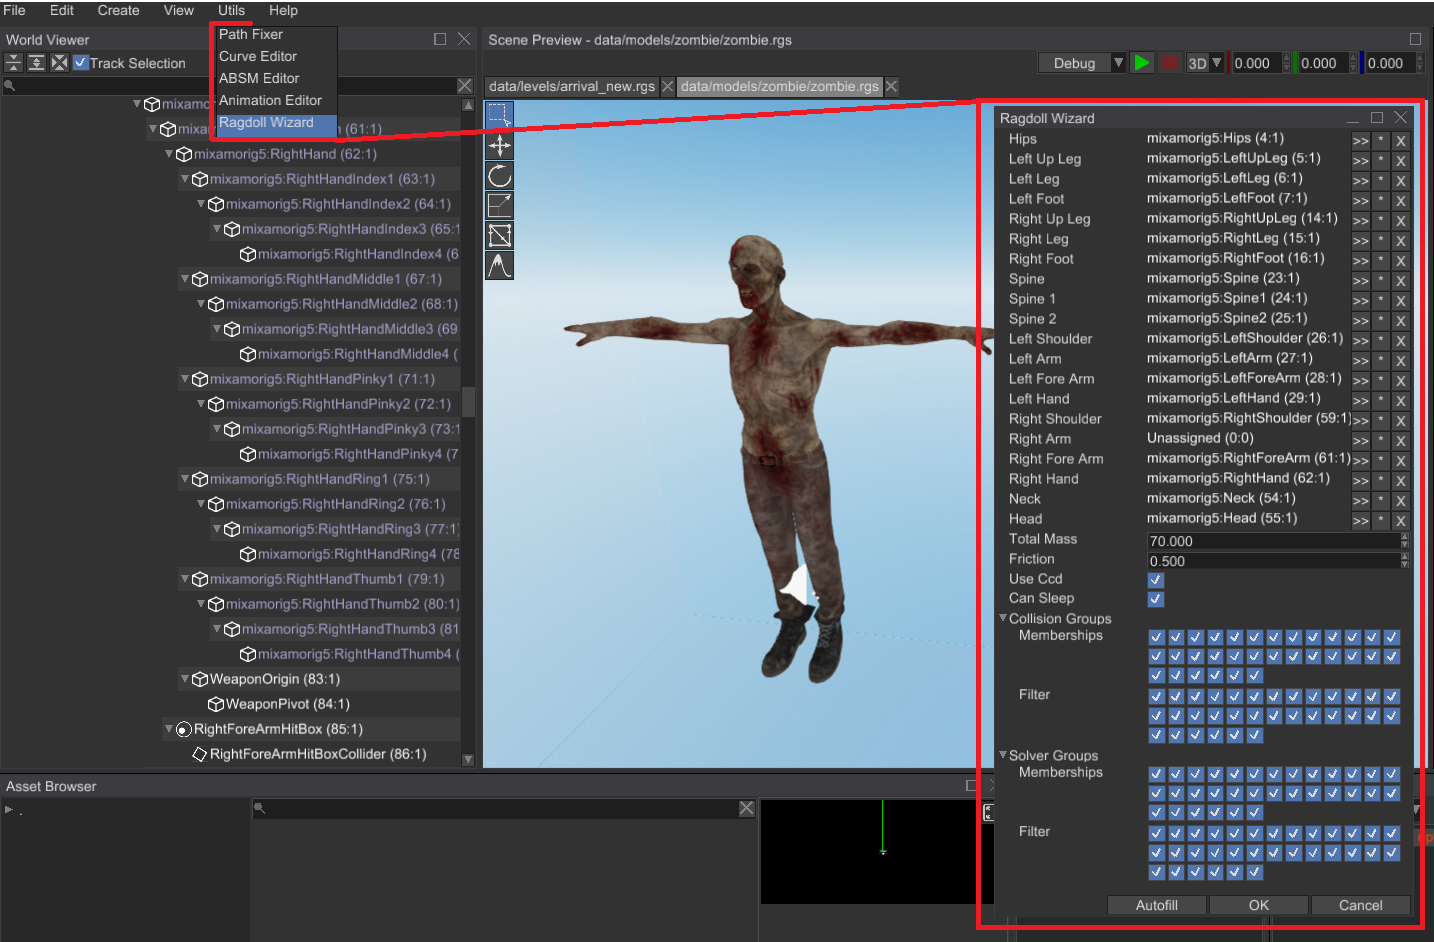
\includegraphics{images/physics_ragdoll.png}
\caption{ragdoll wizard}
\end{figure}

It can be opened from \texttt{Utils} menu and contains quite a lot of node handle fields that needs to be filled. Thankfully, there's an \texttt{Autofill} button, by pressing which, the wizard will try to find respective bones of the skeleton and put their handles in the respective fields in the wizard. For now, it is configured to work with \href{https://www.mixamo.com}{mixamo} skeletons.

Other parameters are listed below:

\begin{itemize}
\tightlist
\item
  \texttt{Total\ Mass} - total mass of the ragdoll, it will be used to configure masses of rigid bodies of body parts.
\item
  \texttt{Use\ CCD} - a flag, that defines whether the continuous collision detection (CCD) for body parts should be used or not.
  It is advised to keep this flag on, otherwise body parts might get stuck or fall through the floor, leading to ``explosive'' ragdoll behaviour.
\item
  \texttt{Can\ Sleep} - a flag, that defines whether the body parts can ``sleep'' or not. Sleep in this case means, that a body part can be excluded from physical simulation if it is not moving for some time.
\item
  \texttt{Collision\ Groups} and \texttt{Solver\ Groups} could be used to configure \href{collider.md\#collision-filtering}{collision filtering}.
  It is very important in case if your character has a physical capsule, that is used to ``standard'' character physics. In this case body parts must ignore physical capsule (and vice versa), otherwise your ragdoll will ``explode''.
\end{itemize}

After everything is filled in, you can click \texttt{OK} button and if everything is correct, you should see a bunch of new scene nodes in the world viewer, located under a \texttt{Ragdoll} scene node:

\begin{figure}
\centering
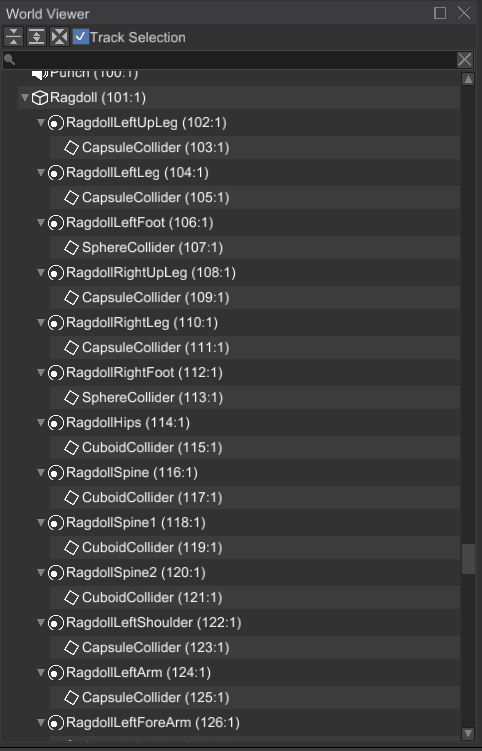
\includegraphics{images/physics_ragdoll2.png}
\caption{ragdoll result}
\end{figure}

As you can see, the amount of entities you'd have to create and configure manually is quite high. Keep in mind, that ragdoll wizard can't generate perfect ragdoll, because of lack of information. The generated ragdoll will most likely require some minor tweaks (mostly joint angular limits).

\subsection{Video Tutorials}\label{video-tutorials}

There's one video tutorial about ragdoll wizard, it also shows the final results in game:

\chapter{Sound System}\label{sound-system}

Fyrox has quite powerful and flexible audio system which will be covered in this chapter. Basic ``building blocks'' are sound sources, sound buffers, audio processing buses with various sound effects, sound context. Read the next chapters to learn more.

\section{Audio Bus}\label{audio-bus}

Audio bus is an audio processing unit that takes audio samples from any number of sound sources and passes them through a chain of effects (zero or more). Processed samples then can be either sent to an audio playback device (speakers, headphones, etc.) or to some other audio bus. There's always one audio bus (primary) that sends its data to an audio playback device, every other audio buses are considered secondary.

\subsection{Graph}\label{graph-1}

As stated above, any audio bus (except primary), can output its audio samples to some other audio bus (primary or secondary). Such relationship forms an audio bus graph:

\begin{figure}
\centering
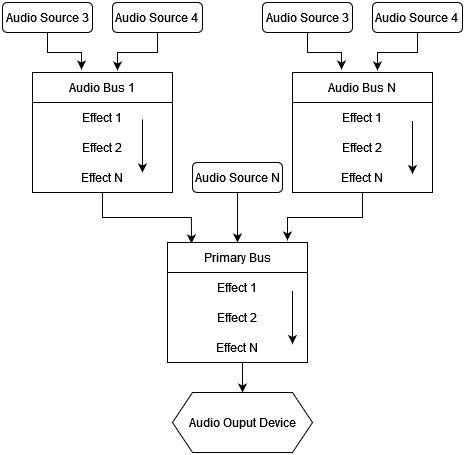
\includegraphics{images/sound_data_flow_diagram.png}
\caption{data flow diagram}
\end{figure}

As you can see, there can be any number of sound sources which attached to the respective audio buses. Each audio bus can have any number of effects (such as lowpass, highpass, etc. filtering; reverb effect and more). Finally, each audio bus is connected to some other audio bus.

Such complex audio processing structure allows you to create pretty much any sound environment. For example, you can create an audio bus with a reverb effect, that will represent a huge hangar with lots of echoes. Then you attach all sound sources located in this ``hangar'' to the audio bus and your sound sources will sound more naturally, according to environment.

\subsection{Effects}\label{effects}

Audio bus can have zero or more audio processing effects. The effects applied one after another (see the arrows on the picture above). You can set any of the following effects:

\begin{itemize}
\tightlist
\item
  \textbf{Attenuation} - changes ``volume'' of input sound samples.
\item
  \textbf{Reverb} - adds echoes, early and late reflections. Could be used to simulate environment with high reflectivity (hangars, parking lots, etc.)
\item
  \textbf{Low Pass Filter} - passes all frequencies below the specified cut-off frequency.
\item
  \textbf{High Pass Filter} - passes all frequencies above the specified cut-off frequency.
\item
  \textbf{Band Pass Filter} - passes all frequencies in a given range around the specified cut-off frequency.
\item
  \textbf{All Pass Filter} - shifts phase of the signal by 90 degrees at the specified cut-off frequency.
\item
  \textbf{Low Shelf Filter} - reduces amplitude of frequencies in a shape like this ̅ \_ at the cutoff frequency.
\item
  \textbf{High Shelf Filter} - reduces amplitude of frequencies in a shape like this \_/̅ at the cutoff frequency.
\end{itemize}

\subsection{Editor}\label{editor-1}

In the editor, audio bus graph is located in the Audio Context panel:

\begin{figure}
\centering
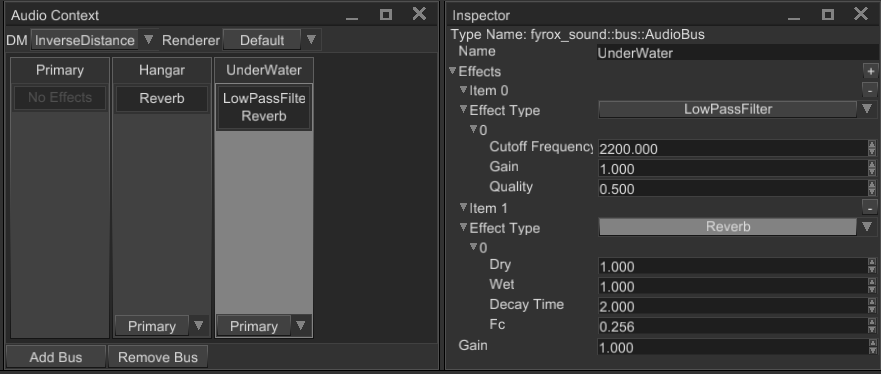
\includegraphics{images/sound_audio_context.png}
\caption{audio context}
\end{figure}

Primary audio bus is located at the left of the panel, every other audio bus is located to the right. Each audio bus (except primary) has a dropdown list (at the bottom), that specifies output audio bus. The list of effect is located in the center; it can be edited in the Inspector (right side of the image).

To attach a sound source to an audio bus, select in the scene and find \texttt{Audio\ Bus} property in the Inspector and set it to the name of desired audio bus.

\section{Sound}\label{sound-1}

In Fyrox, sounds are nodes of type \texttt{Sound}, with all the consequent properties and workflows.

\subsection{How to create}\label{how-to-create-13}

There are two major ways to create sound sources: from the editor and from code.

\subsubsection{From Editor}\label{from-editor}

A sound source could be created from \texttt{Create} menu (or from the same menu by right-clicking on a node in the world viewer):

\begin{figure}
\centering
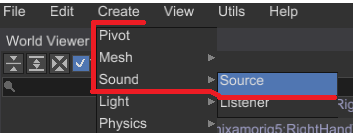
\includegraphics{images/sound_create.png}
\caption{create}
\end{figure}

After the source is created, you can select it and start editing its properties:

\begin{figure}
\centering
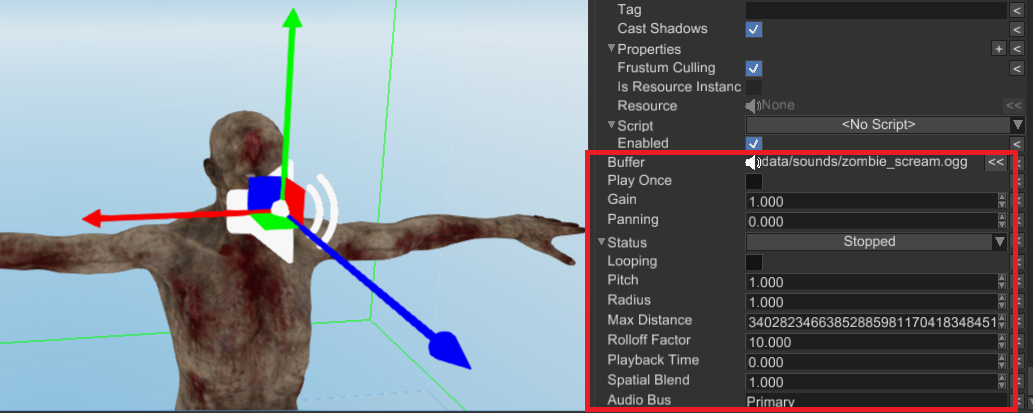
\includegraphics{images/sound_sound.png}
\caption{sound}
\end{figure}

\begin{itemize}
\tightlist
\item
  \texttt{Buffer} - a sound buffer resource, that will be used as a source of samples. If it is empty, then no sound will be
  played. Drag'n'drop a sound resource from the Asset Browser here to assign it to the source.
\item
  \texttt{Play\ Once} - a flag, that defines whether the engine should automatically delete the sound source node from the scene when it is finished playing. Could be useful for one-shot sounds.
\item
  \texttt{Gain} - a numeric value in \texttt{{[}0..1{]}} range, that defines total volume of the sound source. Keep in mind, that this value sets the volume in \emph{linear} scale, while physically-correct approach would be to use logarithmic scale. This will be fixed in future versions.
\item
  \texttt{Panning} - a numeric value in \texttt{{[}-1..1{]}} range, that defines how loud audio channels will be. \texttt{-1} - all the sound will be routed to the left channel, \texttt{1} - to the right channel. This option works only with 2D sounds (whose spatial blend factor is \texttt{0.0})
\item
  \texttt{Status} - a switch with three possible states: \texttt{Stopped}, \texttt{Playing}, \texttt{Paused}. By default, every sound source is in stopped state, do not forget to switch it to the \texttt{Playing} state, otherwise you won't hear anything.
\item
  \texttt{Looping} - a flag, that defines whether the sound source should be playing infinitely, or not. Looping sound source will never switch their status to \texttt{Stopped}.
\item
  \texttt{Pitch} - playback speed multiplier. By default, it is \texttt{1.0} which means default speed.\\
\item
  \texttt{Max\ Distance} - maximum distance, at which the sound source is affected by distance attenuation (for 3D sounds). By default, it set to max possible value. Lower values could be used to prevent sound source from be silent at certain distance.
\item
  \texttt{Rolloff\ Factor} - a numeric value, that defines how fast the volume of the sound source will decay with increasing distance to a listener.
\item
  \texttt{Playback\ Time} - desired time from which the playback should start (in seconds).
\item
  \texttt{Spatial\ Blend} - a numeric value, that defines blending factor between 2D and 3D sound, where \texttt{0.0} - the sound is fully 2D, \texttt{1.0} - the sound is fully 3D. By default, the value is \texttt{1.0}.
\item
  \texttt{Audio\ Bus} - a name of an audio bus, that will be used to process the samples from the sound source. By default, it is set to \texttt{Primary}. It should match the name of some audio bus, that will be used in your scene. More info about audio processing could found \href{bus.md}{here}.
\end{itemize}

\subsubsection{From Code}\label{from-code}

Audio files are loaded using the resource manager:

\begin{Shaded}
\begin{Highlighting}[]
\NormalTok{\{\{\#include ../code/snippets/src/scene/sound.rs:load\_sound\}\}}
\end{Highlighting}
\end{Shaded}

Then, the node is built using the standard builder pattern:

\begin{Shaded}
\begin{Highlighting}[]
\NormalTok{\{\{\#include ../code/snippets/src/scene/sound.rs:build\_sound\_node\}\}}
\end{Highlighting}
\end{Shaded}

There are a few notable things in the example above.

The first is that sounds don't play automatically; in order to do so, we need to invoke \texttt{.with\_status(Status::Playing)}.

The second is that sound nodes are not dropped automatically after playback; dropping it can be performed in two ways. One way is to use the convenient builder API \texttt{.with\_play\_once(true)}; another is to use the graph APIs:

\begin{Shaded}
\begin{Highlighting}[]
\NormalTok{\{\{\#include ../code/snippets/src/scene/sound.rs:sound\_removal\}\}}
\end{Highlighting}
\end{Shaded}

If we want to play background music (or anyway a repeated sound), we just set the \texttt{looping} property when building the node:

\begin{Shaded}
\begin{Highlighting}[]
\NormalTok{\{\{\#include ../code/snippets/src/scene/sound.rs:looping\}\}}
\end{Highlighting}
\end{Shaded}

In order to stream large audio files, instead of loading them entirely in memory, the simplest strategy is to create a corresponding \texttt{.options} file, with the following content:

\begin{Shaded}
\begin{Highlighting}[]
\ErrorTok{(}
  \ErrorTok{stream:} \ErrorTok{true}
\ErrorTok{)}
\end{Highlighting}
\end{Shaded}

If the audio file is called, for example, \texttt{/path/to/background.ogg}, call this \texttt{/path/to/background.ogg.options}.

\subsection{2D and 3D}\label{d-and-3d}

There's no strict separation between 2D and 3D sound sources. The same source could be switched from 2D to 3D (and vice versa) at runtime, by just adjusting \texttt{Spatial\ Blend} property. Spatial blend factor is a numeric value, that defines blending factor between 2D and 3D sound, where \texttt{0.0} - the sound is fully 2D, \texttt{1.0} - the sound is fully 3D. By default, the value is \texttt{1.0} which makes it 3D. Intermediate values could be used to create ``ambisonic'' sound sources - when the source sounds like it is placed at some position in the world, but some part of it is just 2D and does not depend on positioning.

\subsection{Audio bus}\label{audio-bus-1}

It is possible to specify target audio bus to which the sound will output its audio samples. Audio bus is responsible for various audio processing, such as filtering, reverb, etc. To specify output audio bus, just use the \texttt{set\_audio\_bus} method and set the name of an audio bus.

\section{Head Related Transfer Function}\label{head-related-transfer-function}

Head Related Transfer Function (HRTF for short) is special audio processing technique that improves audio spatialization. By default, sound spatialization is very simple - volume of each audio channel (left and right) changes accordingly to orientation of the listener. While this simple and fast, it does not provide good audio spatialization - sometimes it is hard to tell from which direction the actual sound is coming from. To solve this issue, we can use head-related transfer function. Despite its scary, mathematical name, it is easy to understand what it's doing. Instead of uniformly changing volume of all frequencies of the signal (as the naive spatialization does), it changes them separately for each channel. The exact ``gains'' of each frequency of each channel is depends on the contents of head-related transfer function. This is done for each azimuth and elevation angles, which gives full picture of how audio signal from each direction travels to each ear.

HRTF is usually recorded using a head model with ears with a microphone inside each ear. To capture head-related impulse response (time domain) at a fixed distance and angle pair (azimuth and elevation), a very short impulse of sound is produced. Microphones inside each ear records the signal, and then HRIR (time domain) can be converted in HRTF (frequency domain).

\subsection{HRTF on practice}\label{hrtf-on-practice}

The theory above could be boring, however it is very simple to use HRTF on practice. Pick a HRIR sphere from the \href{https://github.com/mrDIMAS/hrir_sphere_builder/tree/master/hrtf_base/IRCAM}{database} (any of *.bin files) and load it in the Audio Context panel:

\begin{figure}
\centering
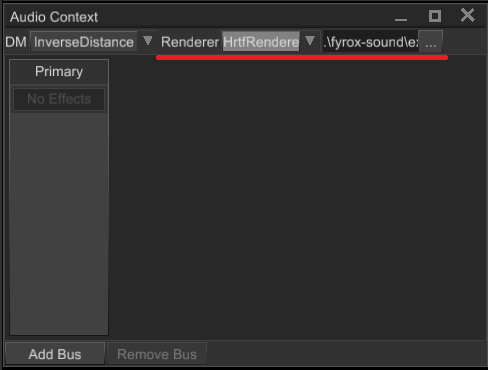
\includegraphics{images/sound_hrtf.png}
\caption{hrtf}
\end{figure}

Once it is loaded, all sounds in the scene will use the HRTF for rendering. The same can be achieved by code:

\begin{Shaded}
\begin{Highlighting}[]
\NormalTok{\# extern crate fyrox;}
\NormalTok{\# use fyrox::scene::\{}
\NormalTok{\#     graph::Graph,}
\NormalTok{\#     sound::\{self, HrirSphere, HrirSphereResource, HrirSphereResourceExt, HrtfRenderer, Renderer\},}
\NormalTok{\# \};}
\NormalTok{\# }
\NormalTok{fn use\_hrtf(graph: \&mut Graph) \{}
\NormalTok{    let hrir\_sphere = HrirSphereResource::from\_hrir\_sphere(}
\NormalTok{        HrirSphere::from\_file("path/to/hrir.bin", sound::SAMPLE\_RATE).unwrap(), "path/to/hrir.bin".into());}
\NormalTok{    graph}
\NormalTok{        .sound\_context}
\NormalTok{        .state()}
\NormalTok{        .set\_renderer(Renderer::HrtfRenderer(HrtfRenderer::new(hrir\_sphere)));}
\NormalTok{\}}
\end{Highlighting}
\end{Shaded}

\subsection{Performance}\label{performance-8}

HRTF is heavy. It is 5-6 times slower than the simple spatialization, so use it only on middle-end or high-end hardware. HRTF performance is linearly dependent on the amount of sound sources: the more sound sources use HRTF, the worse performance will be and vice versa.

\chapter{Animation}\label{animation-4}

Animation allows you to change properties of scene nodes at runtime using a set of key frames. Animation consists of multiple tracks, where each track is bound to a property of a scene node. A track can animate any numeric properties, starting from numbers (including \texttt{bool}) end ending by 2/3/4 dimensional vectors. Each component (number, x/y/z/w vector components) is stored in a \emph{parametric curve}. Every parametric curve contains zero or more \emph{key frames}. Graphically this could be represented like so:

\begin{Shaded}
\begin{Highlighting}[]
\NormalTok{                                         Timeline}
\NormalTok{                                            v}
\NormalTok{  Time   \textgreater{} |{-}{-}{-}{-}{-}{-}{-}{-}{-}{-}{-}{-}{-}{-}{-}|{-}{-}{-}{-}{-}{-}{-}{-}{-}{-}{-}{-}{-}{-}{-}{-}{-}{-}{-}{-}{-}{-}{-}{-}{-}{-}{-}{-}{-}{-}{-}{-}{-}{-}{-}{-}\textgreater{}}
\NormalTok{           |               |}
\NormalTok{  Track1 \textgreater{} | node.position |                                     }
\NormalTok{           |   X curve     |..1..........5...........10..........}
\NormalTok{           |   Y curve     |..2.........{-}2..................1....  \textless{} Curve key frames}
\NormalTok{           |   Z curve     |..1..........9......................4}
\NormalTok{           |\_\_\_\_\_\_\_\_\_\_\_\_\_\_\_|  }
\NormalTok{  Track2   | node.property |                                  }
\NormalTok{           | ............  |.....................................}
\NormalTok{           | ............  |.....................................}
\NormalTok{           | ............  |.....................................}
\end{Highlighting}
\end{Shaded}

Each key frame is just a real number with interpolation mode. Interpolation mode tells the engine how to calculate intermediate values between key frames. There are three kinds of interpolation used in animations (you can skip ``boring math'' if you want):

\begin{itemize}
\tightlist
\item
  \textbf{Constant} - intermediate value will be calculated using leftmost value of two. Constant ``interpolation'' is usually used to create step-like behaviour, the most common case is to ``interpolate'' two boolean values.
\item
  \textbf{Linear} - intermediate value will be calculated using linear interpolation \texttt{i\ =\ left\ +\ (right\ -\ left)\ /\ t}, where \texttt{t\ =\ (time\_position\ -\ left)\ /\ (right\ -\ left)}. \texttt{t} is always in \texttt{0..1} range. Linear interpolation is usually used to create ``straight'' transitions between two values.
\item
  \textbf{Cubic} - intermediate value will be calculated using Hermite cubic spline: \texttt{i\ =\ (2t\^{}3\ -\ 3t\^{}2\ +\ 1)\ *\ left\ +\ (t\^{}3\ -\ 2t\^{}2\ +\ t)\ *\ left\_tangent\ +\ (-2t\^{}3\ +\ 3t\^{}2)\ *\ right\ +\ (t\^{}3\ -\ t\^{}2)\ *\ right\_tangent}, where \texttt{t\ =\ (time\_position\ -\ left)\ /\ (right\ -\ left)} (\texttt{t} is always in \texttt{0..1} range), \texttt{left\_tangent} and \texttt{right\_tangent} is usually a \texttt{tan(angle)}. Cubic interpolation is usually used to create ``smooth'' transitions between two values.
\end{itemize}

\subsection{Web Demo}\label{web-demo}

You can explore animation system capabilities in this \href{https://fyrox.rs/assets/demo/animation/index.html}{web demo}. Keep in mind, that it was designed to run on PC and wasn't tested on mobile devices.

\subsection{Track binding}\label{track-binding}

Each track is always bound to a property in a node, either by its name or by a special binding. The name is used to fetch the property using reflection, the special binding is a faster way of fetching built-in properties. It is usually used to animate position, scale and rotation (these are the most common properties available in every scene node).

\subsection{Time slice and looping}\label{time-slice-and-looping}

While key frames on the curves can be located at arbitrary position in time, animations usually plays a specific time slice. By default, each animation will play on a given time slice infinitely - it is called \emph{animation looping}, it works in both playback directions.

\subsection{Speed}\label{speed}

You can vary playback speed in wide range, by default every animation has playback speed multiplier set to 1.0. The multiplier tells how faster (\textgreater1) or slower (\textless1) the animation needs to be played. Negative speed multiplier values will reverse playback.

\subsection{Enabling or disabling animations}\label{enabling-or-disabling-animations}

Sometimes there's a need to disable/enable an animation or check if it is enabled or not, you can do this by using the pair of respective methods - \texttt{Animation::set\_enabled} and \texttt{Animation::is\_enabled}.

\subsection{Signals}\label{signals}

Signal is a named marker on specific time position on the animation timeline. Signal will emit an event if the animation playback time passes signal's position from left-to-right (or vice versa depending on playback direction). Signals are usually used to attach some specific actions to a position in time. For example, you can have a walking animation and you want to emit sounds when character's feet touch ground. In this case you need to add a few signals at times when each foot touches the ground. After that all you need to do is to fetch animation events one-by-one and emit respective sounds. See respective \href{signal.md}{chapter} for more info.

\subsection{Creating From Code}\label{creating-from-code}

Usually, animations are created from the editor or some external tool and then imported in the engine. Before trying the example below, please read the docs for \texttt{AnimationPlayer} node, it is much more convenient way of animating other nodes. The node can be created from the editor, and you don't even need to write any code. Use the following example code as a guide \textbf{only} if you need to create procedural animations:

\begin{Shaded}
\begin{Highlighting}[]
\NormalTok{\{\{\#include ../code/snippets/src/animation/mod.rs:create\_animation\}\}}
\end{Highlighting}
\end{Shaded}

The code above creates a simple animation that moves a node along X axis in various ways. The usage of the animation is only for the sake of completeness of the example. In the real games you need to add the animation to an animation player scene node, and it will do the job for you.

\subsection{Importing}\label{importing}

It is also possible to import an animation from external source (such as FBX files). You can do this in two major ways: from code or from the editor. The following sections shows how to use both ways.

\subsubsection{From Editor}\label{from-editor-1}

At first, make sure that you have your 3D model instantiated in the scene. The following example has \texttt{agent.fbx} instance in the scene (to do that, just drag'n'drop your 3D model in the scene from the Asset Browser). To import an animation you need to create an \texttt{Animation\ Player} scene node, open the \href{anim_editor.md}{Animation Editor} and click the button with arrow-down icon:

\begin{figure}
\centering
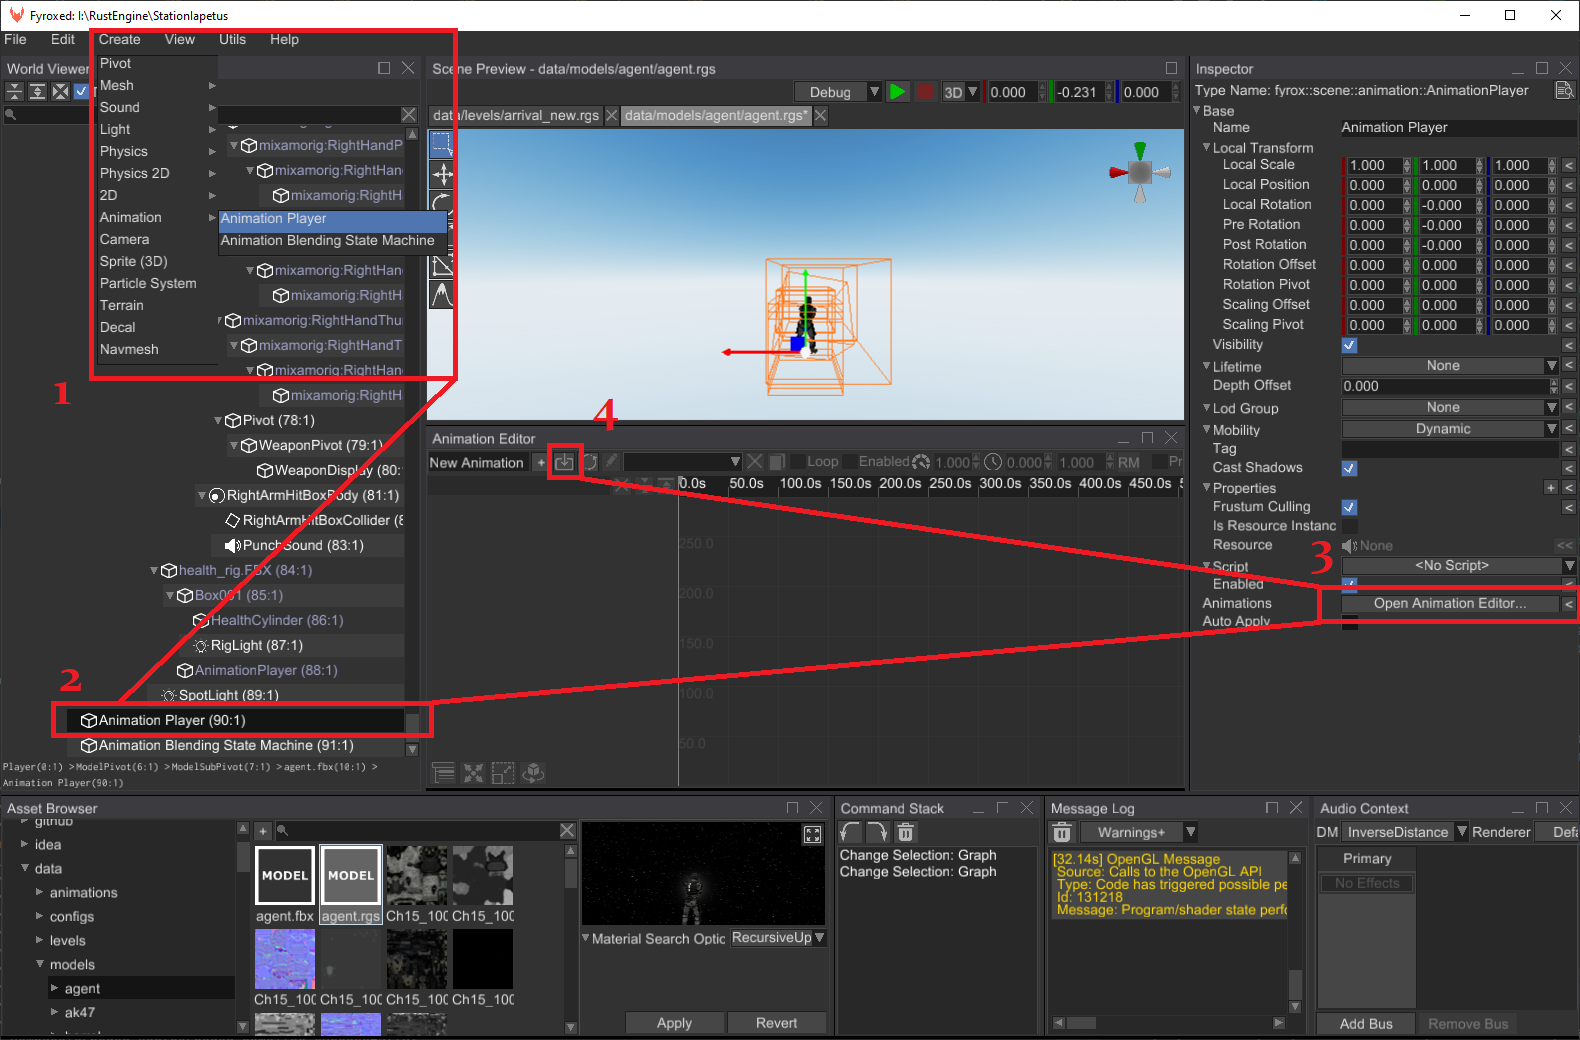
\includegraphics{images/animation/import_animation_1.png}
\caption{Step 1}
\end{figure}

Now you need to pick the root node of your 3D model to which you'll import your animation. Usually it will be called the same as your 3D model (\texttt{agent.fbx} on the screenshot below):

\begin{figure}
\centering
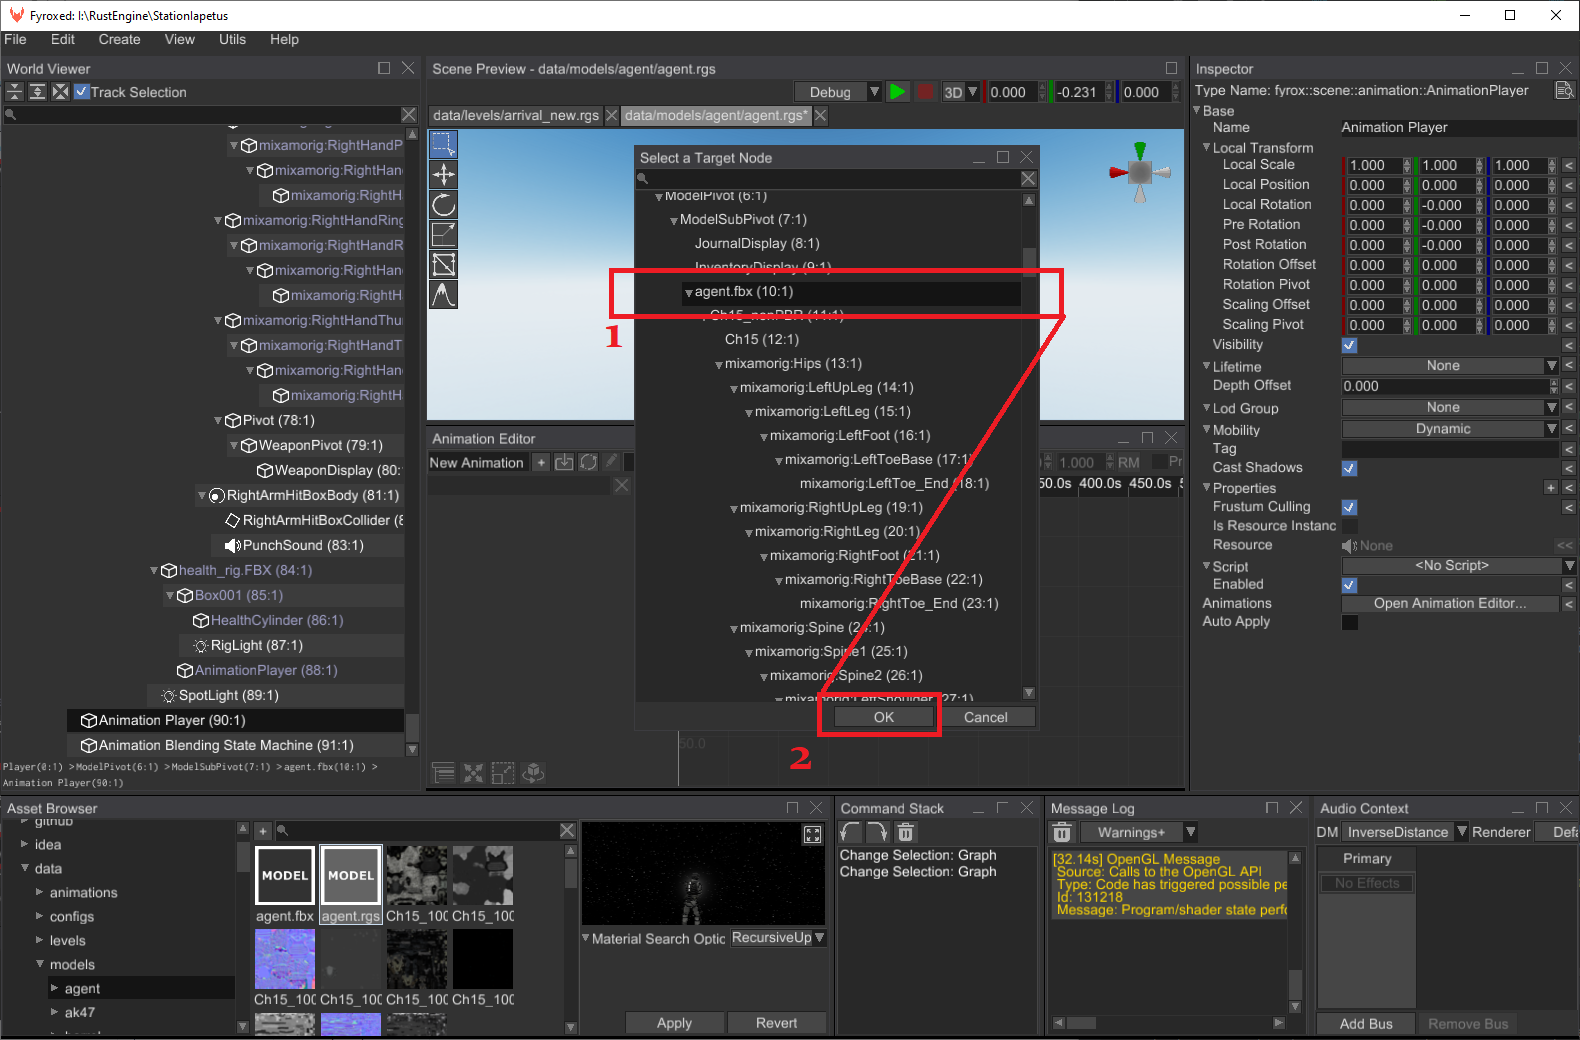
\includegraphics{images/animation/import_animation_2.png}
\caption{Step 2}
\end{figure}

The last thing you need to do is to pick the animation you want to import:

\begin{figure}
\centering
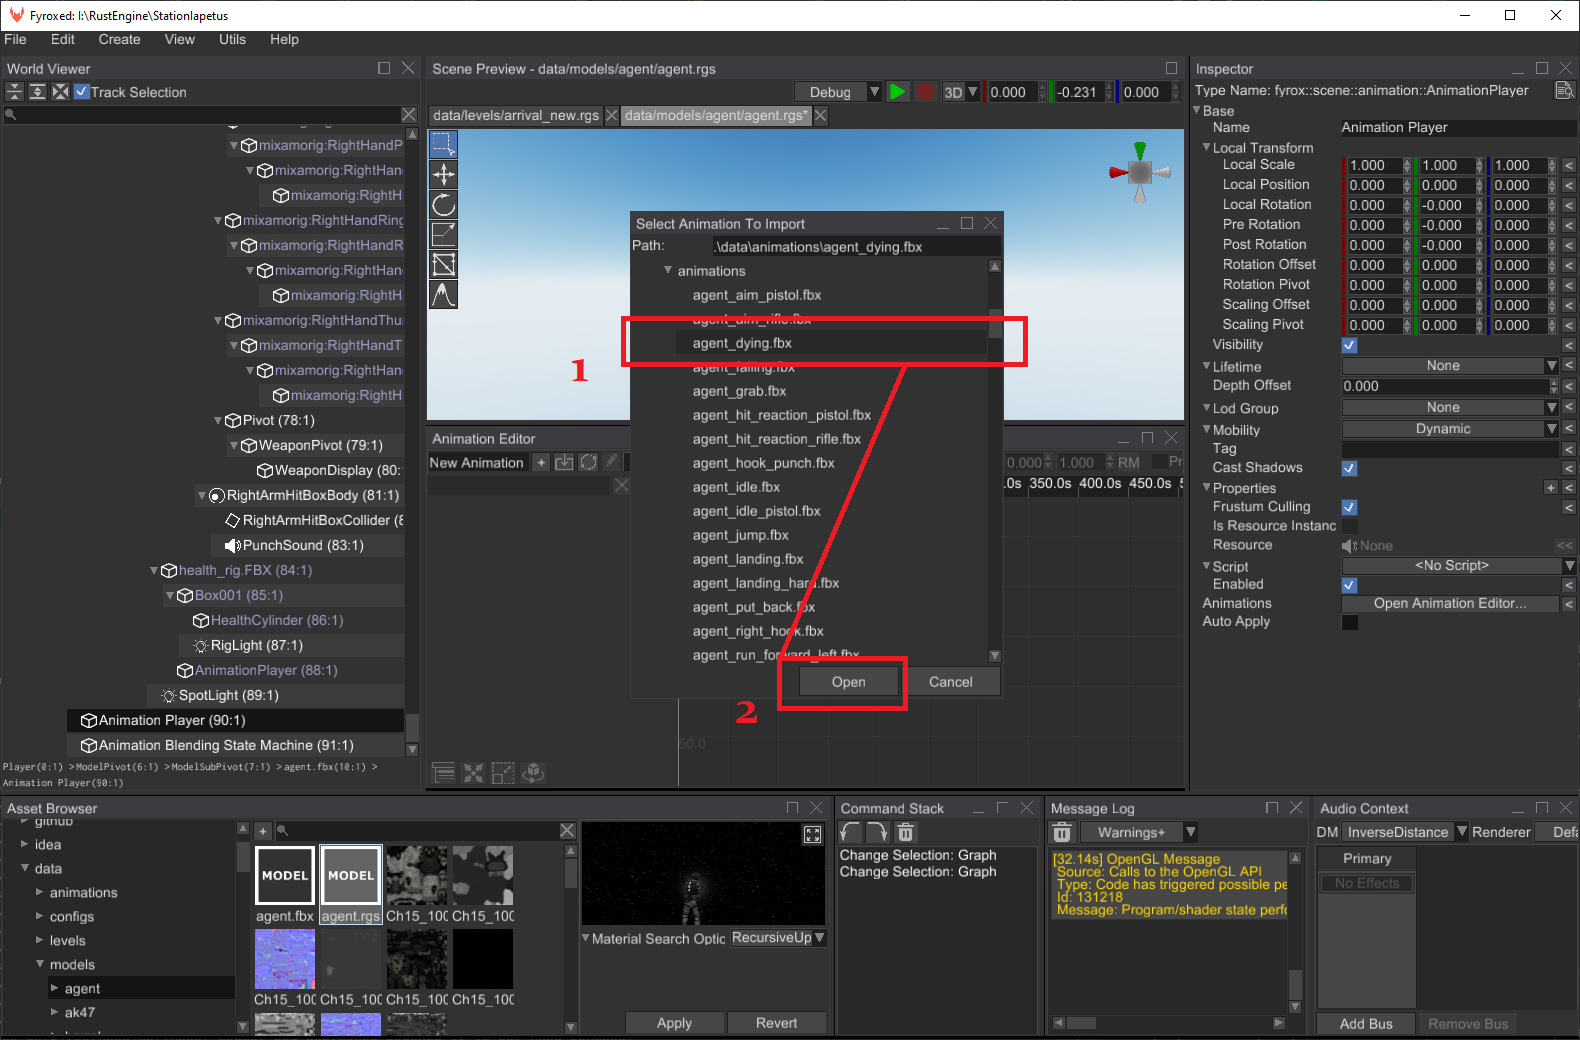
\includegraphics{images/animation/import_animation_3.png}
\caption{Step 3}
\end{figure}

If everything is correct, you can preview your animation by clicking \texttt{Preview} checkbox:

\begin{figure}
\centering
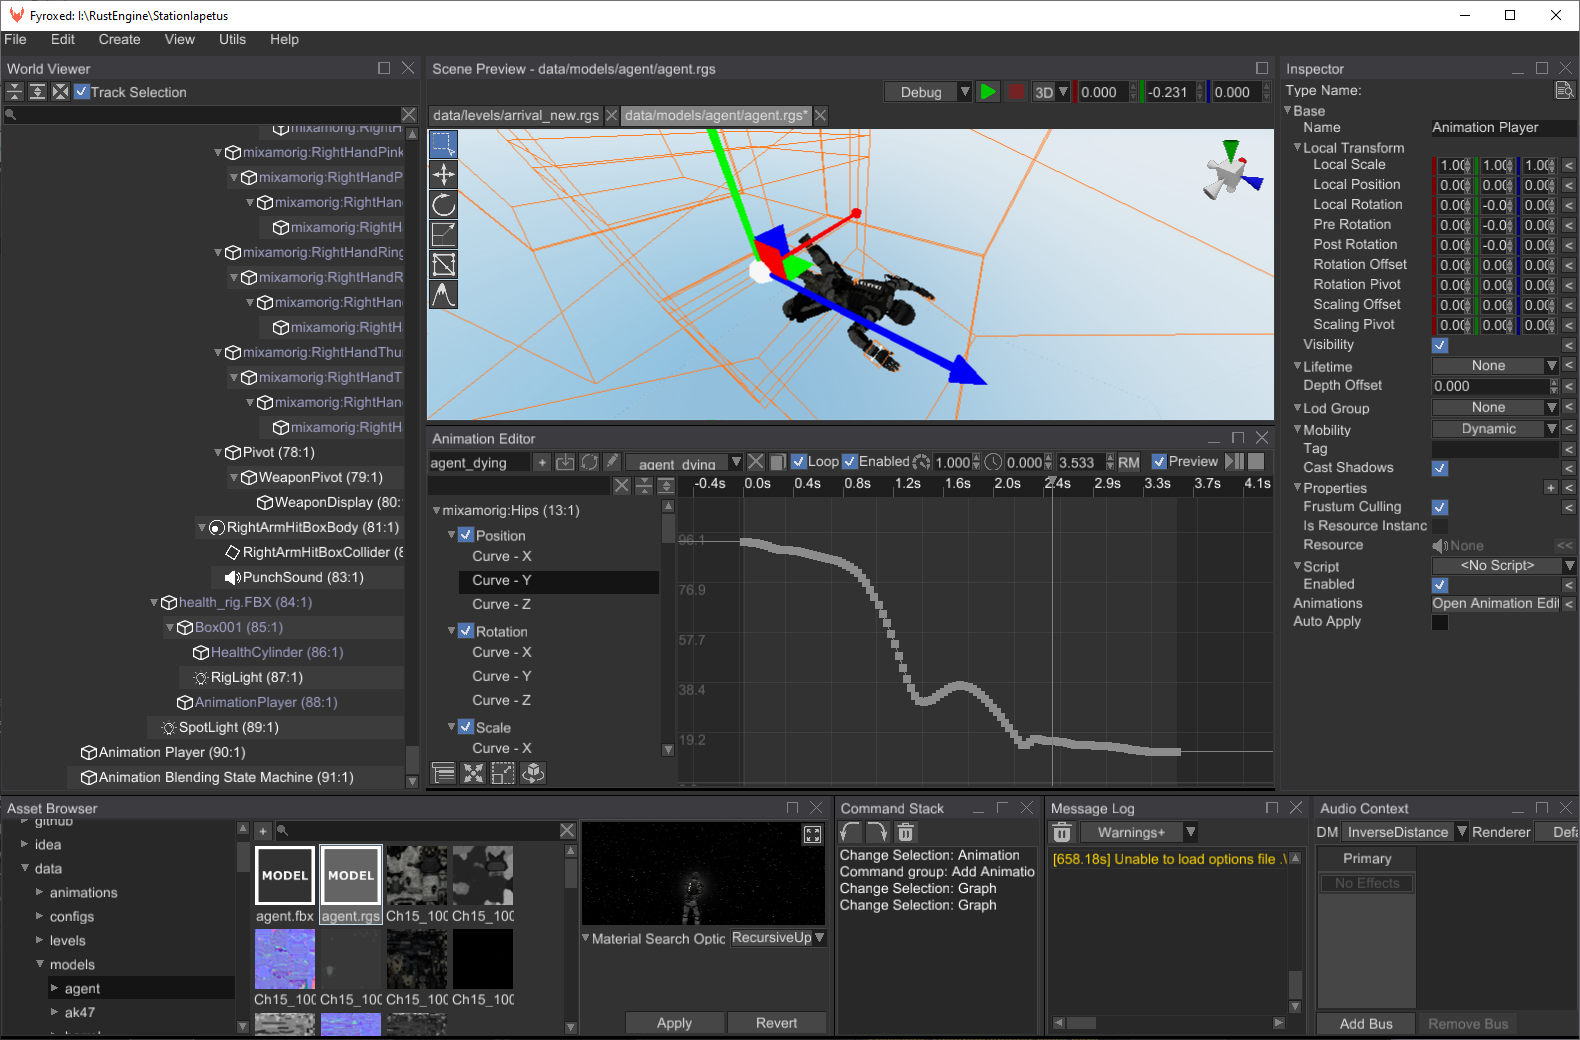
\includegraphics{import_animation_4.png}
\caption{Step 4}
\end{figure}

\subsubsection{From Code}\label{from-code-1}

You can do the same as in the previous section, but from code:

\begin{Shaded}
\begin{Highlighting}[]
\NormalTok{\{\{\#include ../code/snippets/src/animation/mod.rs:create\_animated\_character\}\}}
\end{Highlighting}
\end{Shaded}

As you can see, at first this code creates an instance of a 3D model. Then it loads an animation and creates its instance in the animation player. Please note, that this code uses \texttt{async}, which produces a future which should be driven by some executor. You can use \texttt{block\_on} method to execute it at call site (this won't work on WebAssembly).

It is advised to prefer the editor to code approach, because it hides all this tedious code and properly handles asynchronous loading on all platforms.

\subsection{Playing an Animation}\label{playing-an-animation}

Animations will be played automatically if the respective animation player is has the property \texttt{Auto\ Apply} set to \texttt{true}. Since the animation player can contain multiple animations, all of them will be played at once. You can enable/disable animations when needed by finding them by name from code and switching \texttt{Enabled} property:

\begin{Shaded}
\begin{Highlighting}[]
\NormalTok{\{\{\#include ../code/snippets/src/animation/mod.rs:enable\_animation\}\}}
\end{Highlighting}
\end{Shaded}

This code could also be used to change animation properties at runtime. To do that, replace \texttt{set\_enabled} with some other methods, such as \texttt{set\_speed}, \texttt{set\_loop}, \texttt{set\_root\_motion\_settings} etc.

\section{Animation Editor}\label{animation-editor}

\begin{figure}
\centering
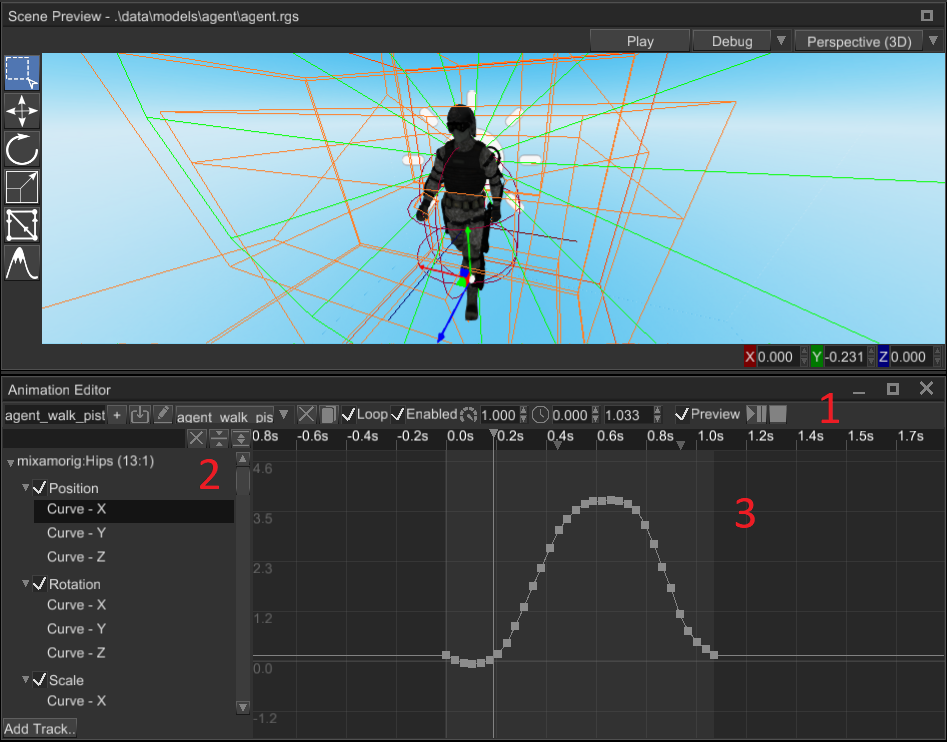
\includegraphics{images/animation/anim_editor.png}
\caption{anim editor}
\end{figure}

Animation Editor is a tool that helps you to create and preview animations. This is a powerful tool that can be used to animate pretty much any numeric property. It has three main parts:

\begin{enumerate}
\def\labelenumi{\arabic{enumi}.}
\tightlist
\item
  \texttt{Toolbar} - contains a set of tools that changes a particular part of an animation (name, length, speed, etc.)
\item
  \texttt{Track\ List} - contains a list of tracks of nodes that will be animated.
\item
  \texttt{Curve\ Editor} - curve editor allows you to edit behaviour of a numeric parameter over the time.
\end{enumerate}

The editor can be opened in two ways - using \texttt{Utils\ -\textgreater{}\ Animation\ Editor} or by selecting an animation player node and clicking \texttt{Open\ Animation\ Editor} button in the inspector.

\begin{figure}
\centering
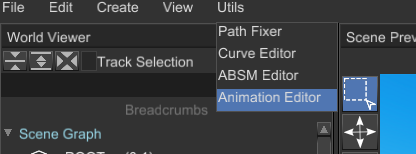
\includegraphics{images/animation/ae_open1.png}
\caption{open1}
\end{figure}

\begin{figure}
\centering
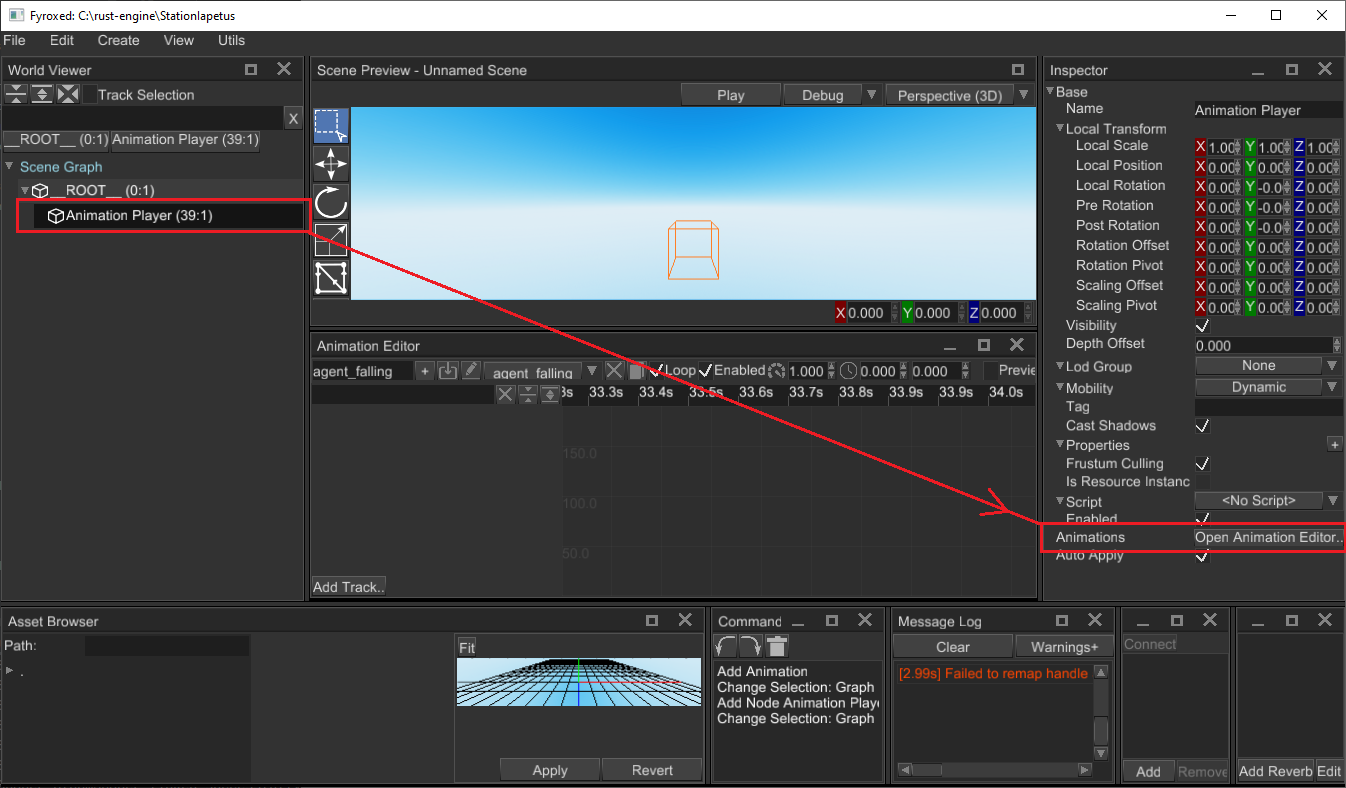
\includegraphics{images/animation/ae_open2.png}
\caption{open2}
\end{figure}

In both ways you still need to select an animation player for editing.

\subsection{Typical Workflow}\label{typical-workflow}

At first, you need to create or \hyperref[animation-importing]{import} an animation, then you need to set its time slice to desired range (see \hyperref[toolbar]{Time Slice} in the section below), then you need to add a few tracks for desired properties and finally add some keys. You can \hyperref[preview-mode]{preview} the results at any time, keep in mind that any attempt to change an animation while it is the preview mode, will revert every change from the preview mode and only then apply your change.

\subsection{Toolbar}\label{toolbar}

The toolbar contains a set of tools that changes a particular part of an animation (name, length, speed, etc.). It looks like this:

\begin{figure}
\centering
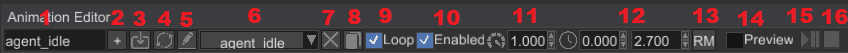
\includegraphics{images/animation/ae_toolbar.png}
\caption{toolbar}
\end{figure}

\begin{enumerate}
\def\labelenumi{\arabic{enumi}.}
\tightlist
\item
  \texttt{Animation\ Name} - name of a currently selected animation.
\item
  \texttt{Add\ Animation} - adds a new empty animation with the name from the text box at the left to the animation player.
\item
  \texttt{Import\ Animation} - starts animation importing process. See \hyperref[animation-importing]{Animation Importing} section for more info.
\item
  \texttt{Reimport\ Animation} - re-imports the animation from an external file, it is useful if you need to change animation's content, while keep references to it valid.
\item
  \texttt{Rename\ Animation} - renames a currently selected animation using the name from the text box at the left.
\item
  \texttt{Animation\ Selector} - allows you to switch currently edited animation.
\item
  \texttt{Delete\ Animation} - deletes a currently selected animation, tries to select last animation from the list if possible.
\item
  \texttt{Duplicate\ Animation} - clones a currently selected animation.
\item
  \texttt{Loop\ Animation} - enables or disables looping of a currently selected animation.
\item
  \texttt{Enable\ Animation} - enables or disables a currently selected animation.
\item
  \texttt{Animation\ Speed} - sets a new playback speed of a currently selected animation.
\item
  \texttt{Time\ Slice} - a time range (in seconds) which defines start and end time of a currently selected animation. The range is highlighted in the curve editor.
\item
  \texttt{Root\ Motion} - open root motion settings. See \hyperref[root-motion]{Root Motion} section for more info.
\item
  \texttt{Preview\ Switch} - enables or disables animation preview. See \hyperref[preview-mode]{\texttt{Preview\ Mode}} section for more info.
\item
  \texttt{Play/Pause} - plays or pauses a currently selected animation (allowed only in the preview mode).
\item
  \texttt{Stop} - stops a currently selected animation (allowed only in the preview mode).
\end{enumerate}

\subsection{Track List}\label{track-list}

The track list contains a list of tracks of nodes that will be animated. It looks like this:

\begin{figure}
\centering
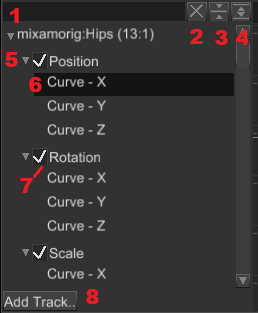
\includegraphics{images/animation/ae_track_list.png}
\caption{track list}
\end{figure}

\begin{enumerate}
\def\labelenumi{\arabic{enumi}.}
\tightlist
\item
  \texttt{Filter\ Bar} - filters the track list by finding tracks whose names matching the filter. You can use this to find tracks that belong to a particular scene node.
\item
  \texttt{Clear\ Filter} - clears the filter, the track list will show all the tracks after this.
\item
  \texttt{Collapse\ All} - collapses all the tracks in the list.
\item
  \texttt{Expand\ All} - expands all the tracks in the list.
\item
  \texttt{Track} - a track with some number of children parametric curves.
\item
  \texttt{Track\ Component\ Curve} - parametric curve that serves a data source for the animation for a particular track.
\item
  \texttt{Track\ Switch} - enables or disables a track; disabled tracks won't ``touch'' their properties.
\item
  \texttt{Add\ Track} - starts property binding process, see \hyperref[property-binding]{Property Binding} section for more info.
\end{enumerate}

\subsubsection{Track Context Menu}\label{track-context-menu}

\begin{figure}
\centering
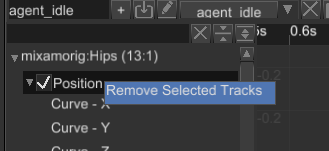
\includegraphics{images/animation/ae_track_context_menu.png}
\caption{context menu}
\end{figure}

\begin{itemize}
\tightlist
\item
  \texttt{Remove\ Selected\ Tracks} - removes selected tracks; you can remove multiple tracks at a time by selecting them while holding \texttt{Ctrl}.
\end{itemize}

\subsection{Curve Editor}\label{curve-editor}

Curve editor allows you to edit parametric curves (one at a time). A curve consists of zero or more key frames with various transition rules between current and the next. The editor looks like this:

\begin{figure}
\centering
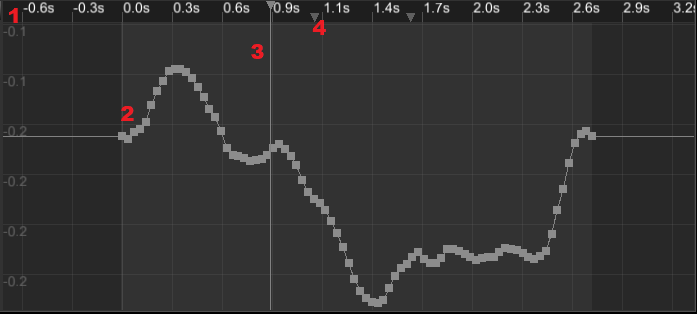
\includegraphics{images/animation/ae_curve_editor.png}
\caption{curve editor}
\end{figure}

\begin{enumerate}
\def\labelenumi{\arabic{enumi}.}
\tightlist
\item
  \texttt{Time\ Ruler} - shows time values and every signal of a currently selected animation. A click on the time ruler will move the playback cursor at the click position. You can move it by clicking at the cursor and moving the mouse while holding the left mouse button. Animation signals can be moved in the same fashion.
\item
  \texttt{Parametric\ Curve} - a curve that defines how a value changes over time.
\item
  \texttt{Time\ Thumb} - animation playback cursor, useful only for preview.
\item
  \texttt{Animation\ Signal} - some animation signal that will produce animation events when the playback cursor passes it.
\end{enumerate}

\subsubsection{Time Ruler Context Menu}\label{time-ruler-context-menu}

\begin{figure}
\centering
\includegraphics{images/animation/ae_time_ruler_context_menu.png}
\caption{time ruler context menu}
\end{figure}

\begin{itemize}
\tightlist
\item
  \texttt{Remove\ Signal} - removes an animation signal under the mouse cursor.
\item
  \texttt{Add\ Signal} - adds a new animation signal at the mouse cursor position.
\end{itemize}

\subsubsection{Key Frame Context Menu}\label{key-frame-context-menu}

\begin{figure}
\centering
\includegraphics{images/animation/ae_key_frame_context_menu.png}
\caption{key frame context menu}
\end{figure}

\begin{itemize}
\tightlist
\item
  \texttt{Location} - shows a key location and allows you to change it. Useful for setting precise values.
\item
  \texttt{Value} - shows a key value and allows you to change it. Useful for setting precise values.
\item
  \texttt{Add\ Key} - adds a new key to the curve.
\item
  \texttt{Remove} - removes all selected keys. You can select multiple keys either by box selection (click and drag the mouse to active box selection) or by clicking on separate keys while holding \texttt{Ctrl}.
\item
  \texttt{Key...} - allows you to change the interpolation type of key. It could be one of the following values: Constant, Linear, Cubic.
\item
  \texttt{Zoom\ To\ Fit} - tries to find zooming values (for both axes) and the view position with which the entire curve fits in the viewport.
\end{itemize}

\subsection{Property Binding}\label{property-binding}

To animate a property all you need to do is to click on \texttt{Add\ Track...} button at the bottom of the track list, select a node to animate and then select a property that will be animated. There are two windows that will be shown one after another:

\begin{figure}
\centering
\includegraphics{images/animation/ae_add_track_select_node.png}
\caption{step1}
\end{figure}

\begin{figure}
\centering
\includegraphics{images/animation/ae_add_track_select_property.png}
\caption{step2}
\end{figure}

You can cancel property binding at any time by clicking \texttt{Cancel} in any of the windows. Keep in mind that you can animate only numeric properties, so not every property is shown in the window.

\subsection{Animation Importing}\label{animation-importing}

Animations can be stored in separate files, but the engine requires all of them to be in a single Animation Player. To put an animation from an external resource (an FBX, for instance) in the animation player you can use animation importing. To do that, click on animation import icon and then select a root node of the hierarchy that is animated in the external animation file, then select the animation file and click \texttt{Ok}. The engine will try to import the animation and map it to the given hierarchy, mapping is done using node names, so animated node names must match in both your scene and your external animation file.

\begin{figure}
\centering
\includegraphics{images/animation/ae_import_select_target_node.png}
\caption{step1}
\end{figure}

\begin{figure}
\centering
\includegraphics{images/animation/ae_import_select_animation.png}
\caption{step2}
\end{figure}

Content of existing animations can be replaced by reimporting. Click on a button with two circular arrows to reimport your animation. It could be useful if you changed your animation in some external editor (Blender for example) and want to apply changes in your game.

\subsection{Preview Mode}\label{preview-mode}

Preview mode helps you to see and debug your animation. After activating the mode, you need to play the animation by clicking the \texttt{Play/Pause} button:

\begin{figure}
\centering
\includegraphics{images/animation/anim_editor.gif}
\caption{anim editor}
\end{figure}

Any significant change made in the scene will automatically deactivate the preview mode reverting all the changes made by playing animation.

\subsection{Root Motion}\label{root-motion}

See \href{root_motion/root_motion.md}{Root Motion chapter} for more info.

\subsection{Limitations}\label{limitations-2}

For now there's no dopesheet mode in the editor, you can edit only one numeric parameter at a time. Also, there's no capture mode - this is a special mode in which the editor automatically adds your changes in the scene to the animation. These limitations will be removed in the future versions.

\section{Animation Blending}\label{animation-blending}

Animation blending is a powerful feature that allows you to mix multiple animations into one. Each animation is mixed with a various weights which in sum gives 1.0 (100\%). By having opposite coefficients (k1 = 0 -\textgreater{} 1, k2 = 1 -\textgreater{} 0) changing in time it is possible to create transition effect.

Handling transitions with all the coefficients is a routine job, the engine can handle it for you giving you some nice
features:

\begin{itemize}
\tightlist
\item
  Multiple states with smooth transitions between them
\item
  Ability to blend multiple animations in one and use it as pose source for blending
\item
  Ability to specify a set of variables that will be used as blending coefficients and transition rules.
\end{itemize}

All these features consolidated in so-called animation blending state machine (ABSM). Machine is used to blend multiple animation as well as perform automatic ``smooth'' transition between states. In general, ABSM could be represented like this:

\begin{figure}
\centering
\includegraphics{absm_structure.png}
\caption{ABSM Structure}
\end{figure}

At the first look it may seem very complicated, but in reality it uses quite simple techniques. Let's start from the left side of the picture and go to the right. Yellow rectangle at the left depicts an animation player node that contains a bunch of animations, that will be used for blending. Two center blocks (layer 0 and layer 1) depicts separate layers (ABSM could have any number of layers in it). Each layer can contain an arbitrary nodes (green shapes), states (blue shapes), transitions (thick yellow arrows).

Nodes serves as a source of poses, that can be blended in any desired way. States are the part of the inner state machine, only one state could be active at the same time. Transitions are used to specify state transition rules.

At the ``exit'' of each layer there's a layer filter, it is responsible for filtering out values for specific scene nodes and could be used to prevent some scene nodes from being animated by a certain layer. Please note that despite the look of it, layer filter not necessarily be applied after all animations and states are blended - it could be done at any moment and drawn like so only for simplicity reasons.

The last, but not the least, important thing on the picture is the parameters container on the right side of the picture. Parameter either a transition rule, blending weight, or sampling point. If you look closely at the transitions or animation blending nodes you'll see small text marks. This is the names of the respective parameters.

In general, any state machine works like this - ABSM nodes are used to blend or fetch animations and their resulting poses are used by ABSM states. Active state provides final pose, which is then passes filtering and returned to you. After the last stage, you can apply the pose to a scene graph to make the resulting animation to have effect.

\subsection{How to create}\label{how-to-create-14}

As always, there are two major ways of creating things in Fyrox - from the editor or from code. Take your pick.

\subsection{From editor}\label{from-editor-2}

Use \href{absm_editor.md}{ABSM Editor} for to create animation blending state machines.

\subsection{From code}\label{from-code-2}

You can always create an ABSM from code, a simple ABSM could be created like this:

\begin{Shaded}
\begin{Highlighting}[]
\NormalTok{\{\{\#include ../code/snippets/src/animation/blending.rs:create\_absm\}\}}
\end{Highlighting}
\end{Shaded}

Here we have Walk, Idle and Run states which use different sources of poses:
- Walk - is the most complicated here - it uses result of blending between \texttt{Aim} and \texttt{Walk} animations with different weights. This is useful if your character can only walk or can walk \emph{and} aim at the same time. Desired pose determined by Walk Weight and Aim Weight parameters combination.
- Run and idle both directly use animation as pose source.

There are four transitions between three states each with its own rule. Rule is just a boolean parameter that indicates that transition should be activated. Let's look at the code example of the above state graph:

As you can see, everything is quite straightforward. Even such simple state machine requires quite a lot of code, which can be removed by using ABSM editor. Read the next chapter to learn about it.

\section{Animation Blending State Machine (ABSM) Editor}\label{animation-blending-state-machine-absm-editor}

While it is possible to create and manage animation blending and state manually from code, it quickly becomes too annoying and hardly manageable. To help you create and manage blending machines in easy way, the engine offers an ABSM Editor tool. This chapter is an overview of the editor, it is quite complex, but the guide should help you to figure out which part is made for what. Next chapter will help you to create your first animation blending state machine.

\begin{figure}
\centering
\includegraphics{images/animation/absm.png}
\caption{absm editor}
\end{figure}

The editor has four main parts (panels):

\begin{enumerate}
\def\labelenumi{\arabic{enumi}.}
\tightlist
\item
  \texttt{Toolbar} - contains a set of tools to edit animation layers and enable/disable preview mode. See \hyperref[toolbar]{Toolbar} section for more info.
\item
  \texttt{Parameters} - allows you to edit various variables that are responsible for transitions, weight parameters for blending, etc. See \href{./absm_parameters.png}{Parameters} section for more info.
\item
  \texttt{State\ Graph} - allows you to create, delete, edit states and transition between them. See \hyperref[state-graph]{State Graph} section for more info.
\item
  \texttt{State\ Viewer} - allows you to edit pose source for a state. Pose source can be represented either by a single node that plays an animation, or a series of play animation nodes connected to blending nodes (which can be connected to other blending nodes, etc.). See \hyperref[state-viewer]{State Viewer} section for more info.
\end{enumerate}

The editor can be opened in two ways - using \texttt{Utils\ -\textgreater{}\ ABSM\ Editor} or by selecting an animation blending state machine node and clicking \texttt{Open\ ABSM\ Editor...} button:

\begin{figure}
\centering
\includegraphics{images/animation/absm_open1.png}
\caption{open1}
\end{figure}

\begin{figure}
\centering
\includegraphics{images/animation/absm_open2.png}
\caption{open1}
\end{figure}

In both ways you still need to select an an animation blending state machine node for editing.

\subsection{Toolbar}\label{toolbar-1}

\begin{figure}
\centering
\includegraphics{images/animation/absm_toolbar.png}
\caption{toolbar}
\end{figure}

\begin{enumerate}
\def\labelenumi{\arabic{enumi}.}
\tightlist
\item
  \texttt{Preview\ Switch} - enables or disables preview mode for the ABSM. See \hyperref[preview-mode]{Preview Mode} section for more info.
\item
  \texttt{Layer\ Name} - name of the selected layer. Type a new name here to rename currently selected layer (hit enter or just click elsewhere to rename).
\item
  \texttt{Add\ Layer} - adds a new layer with the name in the \texttt{Layer\ Name} text box to the ABSM. ABSM can have multiple layers with the same name, but it strongly advised to set unique names here.
\item
  \texttt{Remove\ Current\ Layer} - removes currently selected layer. You can delete all layers, but in this case your ABSM won't have any effect.
\item
  \texttt{Layer\ Selector} - allows you to select a layer for editing, default selection is none.
\item
  \texttt{Layer\ Mask} - opens a \texttt{Layer\ Mask\ Editor} and helps you to edit the layer mask of the current layer. See
  \hyperref[layer-mask]{Layer Mask} section for more info.
\end{enumerate}

\subsection{Parameters}\label{parameters}

Parameter is a named and typed variable that provides the animation system with some data required for it to work. There are only three type of parameters:

\begin{itemize}
\tightlist
\item
  \texttt{Rule} - boolean value that used as a trigger for transitions. When transition is using some rule, it checks the value of the parameter and if it is \texttt{true} transition starts.
\item
  \texttt{Weight} - real number (\texttt{f32}) that is used a weight when you're blending multiple animations into one.
\item
  \texttt{Index} - natural number (\texttt{i32}) that is used as an animation selector.
\end{itemize}

\begin{figure}
\centering
\includegraphics{images/animation/absm_parameters.png}
\caption{parameters}
\end{figure}

\begin{enumerate}
\def\labelenumi{\arabic{enumi}.}
\tightlist
\item
  \texttt{Add\ Parameters} - adds a new parameter to the parameters' container.
\item
  \texttt{Remove\ a\ Parameter} - removes selected parameter from the parameters' container.
\item
  \texttt{Parameter\ Name} - allows you to set a parameter name.
\item
  \texttt{Parameter\ Type} - allows you to select the type of the parameter.
\item
  \texttt{Parameter\ Value} - allows you to set parameter value.
\end{enumerate}

\subsection{State Graph}\label{state-graph}

State Graph allows you to create states and transitions between them.

\begin{figure}
\centering
\includegraphics{images/animation/absm_state_graph.png}
\caption{state graph}
\end{figure}

\begin{enumerate}
\def\labelenumi{\arabic{enumi}.}
\tightlist
\item
  \texttt{State} - state is final animation for a set of scene nodes, only one state can be active at a time.
\item
  \texttt{Transition} - is an \emph{ordered} connection between two states, it defines how much time it needed to perform blending of two states.
\item
  \texttt{Root\ State} - is an entry state of the current layer.
\end{enumerate}

\subsubsection{State Context Menu}\label{state-context-menu}

\begin{figure}
\centering
\includegraphics{images/animation/absm_state_context_menu.png}
\caption{state context menu}
\end{figure}

\begin{itemize}
\tightlist
\item
  \texttt{Create\ Transition} - starts transition creation from the current state to some other.
\item
  \texttt{Remove} - removes the state.
\item
  \texttt{Set\ As\ Entry\ State} - marks the state as an entry state (this state will be active at beginning).
\end{itemize}

\subsubsection{Transition Context Menu}\label{transition-context-menu}

\begin{figure}
\centering
\includegraphics{images/animation/absm_transition_context_menu.png}
\caption{transition context menu}
\end{figure}

\begin{itemize}
\tightlist
\item
  \texttt{Remove\ Transition} - removes selected transition.
\end{itemize}

\subsubsection{State Properties}\label{state-properties}

Select a \texttt{State} node to edit the following properties:

\begin{figure}
\centering
\includegraphics{images/animation/absm_state_properties.png}
\caption{state properties}
\end{figure}

\begin{itemize}
\tightlist
\item
  \texttt{Position} - is a location of the state on the canvas.
\item
  \texttt{Name} - name of the state.
\item
  \texttt{Root} - handle of the backing animation node inside the state.
\end{itemize}

\subsubsection{Transition Properties}\label{transition-properties}

Select a \texttt{Transition} node to edit the following properties:

\begin{figure}
\centering
\includegraphics{images/animation/absm_transition_properties.png}
\caption{transition properties}
\end{figure}

\begin{itemize}
\tightlist
\item
  \texttt{Name} - name of the state.
\item
  \texttt{Transition\ Time} - amount of time for blending between two states (in seconds).
\item
  \texttt{Elapsed\ Time} - starting amount of blending time.
\item
  \texttt{Source} - handle of a source state.
\item
  \texttt{Desc} - handle of a destination state.
\item
  \texttt{Rule} - a name of \texttt{Rule} type parameter that defines whether the transition can be activated or not.
\item
  \texttt{Invert\ Rule} - defines whether to invert the value of \texttt{Rule} or not.
\item
  \texttt{Blend\ Factor} - defines a percentage (in \texttt{0..1} range) of how much transition was active.
\end{itemize}

\subsection{State Viewer}\label{state-viewer}

State Viewer allows you to edit contents of states. You can create animation blending chains of any complexity, the simplest content of a state is just a single \texttt{Play\ Animation} node. Currently, the engine supports just three animation blending nodes:

\begin{itemize}
\tightlist
\item
  \texttt{Play\ Animation} - takes animation pose directly from specified animation, does nothing to it.
\item
  \texttt{Blend\ Animations} - takes multiple animation poses from respective animations and blends them together with respective blend weights.
\item
  \texttt{Blend\ Animations\ By\ Index} - takes multiple animation poses from respective animations and switches between them with ``smooth'' transition using an index parameter.
\end{itemize}

\begin{figure}
\centering
\includegraphics{images/animation/absm_state_viewer.png}
\caption{state viewer}
\end{figure}

\begin{enumerate}
\def\labelenumi{\arabic{enumi}.}
\tightlist
\item
  \texttt{Node} - is a source of animation for blending.
\item
  \texttt{Connection} - defines how nodes are connected to each other. To create a new connection, click on a small dot on a node, hold the button and start dragging to a dot on some other node.
\item
  \texttt{Root\ Node} - root node is marked green; root node is a final source of animation for the parent state.
\end{enumerate}

\subsubsection{\texorpdfstring{\texttt{Play\ Animation} Properties}{Play Animation Properties}}\label{play-animation-properties}

Select a \texttt{Play\ Animation} node to edit the following properties:

\begin{figure}
\centering
\includegraphics{images/animation/absm_play_animation_properties.png}
\caption{play animation properties}
\end{figure}

\begin{itemize}
\tightlist
\item
  \texttt{Position} - is a location of the node on the canvas.
\item
  \texttt{Animation} - an animation to fetch the pose from.
\end{itemize}

\subsubsection{\texorpdfstring{\texttt{Blend\ Animations} Properties}{Blend Animations Properties}}\label{blend-animations-properties}

Select a \texttt{Blend\ Animations} node to edit the following properties:

\begin{figure}
\centering
\includegraphics{images/animation/absm_blend_animations_properties.png}
\caption{blend animations properties}
\end{figure}

\begin{itemize}
\tightlist
\item
  \texttt{Position} - is a location of the node on the canvas.
\item
  \texttt{Pose\ Sources} - a set of input poses. To add a pose either click on \texttt{+} or \texttt{+Input} on the node itself. Don't forget to connect some nodes to the new input poses.

  \begin{itemize}
  \tightlist
  \item
    \texttt{Weight} - a weight of the pose; could be either a constant value or some parameter.
  \end{itemize}
\end{itemize}

\subsubsection{\texorpdfstring{\texttt{Blend\ Animations\ By\ Index} Properties}{Blend Animations By Index Properties}}\label{blend-animations-by-index-properties}

Select a \texttt{Blend\ Animations\ By\ Index} node to edit the following properties:

\begin{figure}
\centering
\includegraphics{images/animation/absm_blend_animations_by_index_properties.png}
\caption{blend animations by index properties}
\end{figure}

\begin{itemize}
\tightlist
\item
  \texttt{Position} - is a location of the node on the canvas.
\item
  \texttt{Index\ Parameter} - a name of an indexing parameter (must be \texttt{Index} type).
\item
  \texttt{Inputs} - a set of input poses. To add a pose either click on \texttt{+} or \texttt{+Input} on the node itself. Don't forget to
  connect some nodes to the new input poses.

  \begin{itemize}
  \tightlist
  \item
    \texttt{Blend\ Time} - defines how much time is needed to transition to the pose.
  \end{itemize}
\end{itemize}

\subsubsection{Connection Context Menu}\label{connection-context-menu}

Every connection has a context menu that can be shown by a right-click on a connection.

\begin{figure}
\centering
\includegraphics{images/animation/absm_connection_context_menu.png}
\caption{connection context menu}
\end{figure}

\begin{itemize}
\tightlist
\item
  \texttt{Remove\ Connection} - removes the connection between parent nodes.
\end{itemize}

\subsubsection{Node Context Menu}\label{node-context-menu}

Every node has a context menu that can be shown by a right-click on a connection.

\begin{figure}
\centering
\includegraphics{images/animation/absm_node_context_menu.png}
\caption{node context menu}
\end{figure}

\begin{itemize}
\tightlist
\item
  \texttt{Set\ As\ Root} - sets the node as the final pose source of the parent state.
\item
  \texttt{Remove} - removes the node from the state.
\end{itemize}

\subsection{Layer Mask}\label{layer-mask}

\begin{figure}
\centering
\includegraphics{images/animation/absm_layer_mask.png}
\caption{layer mask}
\end{figure}

Layer mask editor allows you to select which nodes \textbf{won't} be animated by the current animation layer. Selected nodes are marked with dark color. To select multiple nodes at once, hold \texttt{Ctrl} and click on items. The text box at the top of the window allows you to search for a particular scene node. To save edited layer mask click \texttt{OK}.

\subsection{Preview Mode}\label{preview-mode-1}

Preview mode turns on the animation blending state machine and its animation player and allows you to see the result of the work of the machine. Any significant changes in the scene automatically disables the preview mode and any changes done by the machine is discarded. While the preview mode is active, you can freely change the values of the parameters to see how the machine will react to this. This helps you to debug your state machine, it is especially useful for complex state machines with lots of layers. Here's how the preview mode works:

\begin{figure}
\centering
\includegraphics{images/animation/absm.gif}
\caption{absm}
\end{figure}

\section{Signals}\label{signals-1}

In some cases you may need to perform an action when at certain time of your animation. It could be a footstep sound, when foot touches ground, grenade tossing, etc. This could be done via animation signals. Animation signal is just a named marker that has time position at an animation timeline. It will be emitted when animation playback time passes it (left-to-right or right-to-left depending on the actual speed of your animation). All you need to do, is to catch these signals in your game code and do the desired actions.

\subsection{How to add}\label{how-to-add}

As usual, there are two possible ways of adding animation signals - from the animation editor and from code.

\subsubsection{From animation editor}\label{from-animation-editor}

To add a signal to some animation, select an animation player, open the animation editor, select some animation in it. Now all you need to do is to right-click on the timeline and press \texttt{Add\ Signal}.

\begin{figure}
\centering
\includegraphics{images/animation/signal_add.png}
\caption{Add Signal}
\end{figure}

After the signal is added, you can select it and edit its properties in the inspector. Also, you can drag it on the timeline to adjust its position.

\begin{figure}
\centering
\includegraphics{images/animation/signal_edit.png}
\caption{Edit Signal}
\end{figure}

Set a meaningful name to the signal, and it is pretty much done - all you need to do next is to write signal handling code in your game. See \hyperref[reacting-to-signal-events]{the next section} to learn how to do it.

\subsubsection{From code}\label{from-code-3}

A signal could also be added from code, this requires knowing a handle of your animation player and a name/handle of your animation. Please note the comment about signal's uuid in the code below.

\begin{Shaded}
\begin{Highlighting}[]
\NormalTok{\{\{\#include ../code/snippets/src/animation/signal.rs:add\_signal\}\}}
\end{Highlighting}
\end{Shaded}

\subsection{Reacting to signal events}\label{reacting-to-signal-events}

When you have your signals ready for use, all you need to do is to react to the signals somehow. This is very simple: just borrow your animation from the animation player and pop animation event one-by-one from internal queue:

\begin{Shaded}
\begin{Highlighting}[]
\NormalTok{\{\{\#include ../code/snippets/src/animation/signal.rs:react\_to\_signal\_events\}\}}
\end{Highlighting}
\end{Shaded}

You can do pretty much anything when reacting to signals. For example, this could be a prefab instantiation to create smoke effect under the feet, playing a footstep sound, etc.

\subsection{Events from ABSM}\label{events-from-absm}

Animation blending state machines are able to collect events from the currently playing animations using different strategies. This ability prevents you from tedious manual animation events collection from a bunch of animations manually.

\begin{Shaded}
\begin{Highlighting}[]
\NormalTok{\{\{\#include ../code/snippets/src/animation/signal.rs:collect\_events\_from\_absm\}\}}
\end{Highlighting}
\end{Shaded}

This function collects all animation events from all active animations in the specified ABSM (in its first layer). The arguments to it are the following:

\begin{itemize}
\tightlist
\item
  \texttt{absm} - a handle to an animation blending state machine node.
\item
  \texttt{strategy} - event collection strategy, which includes all events collection, max and min weight. The last two may be used if you're getting a lot of events and want to get events from the animations with max or min weights respectively.
\item
  \texttt{ctx} - current script context, available in pretty much any script methods.
\end{itemize}

\section{Root Motion}\label{root-motion-1}

Root motion is a special technique that transfers motion from some node in a hierarchy to a physical capsule, which is then used to perform the actual motion. In action it looks like this:

As you can see in the first part of the video, the movement of the character looks more like floating above the ground. This happens because the actual movement of the physical capsule is not synchronized with the movement of the character. Root motion fixes exactly this issue by taking the motion of some root node of the animated hierarchy (hips in case of this character) and transferring it to the physical capsule. This makes the actual movement to be fully synchronized with the movement ``baked'' in the animation.

Root motion also have some nice effect - you can move your character solely by the movement from animation, and it will work perfectly in 99\% of cases. Animations can also contain some rotations which can also be extracted and applied to the physical capsule. The next awesome property is that your character will never stand out of its physical capsule, which will prevent phasing it into walls when playing animations with large movements.

In general, you should prefer root motion -driven movement for your characters whenever you can. Simply because it eliminates a lot of common problems with character movement. It can also be applied to 2D world and will work exactly the same.

\subsection{How to enable}\label{how-to-enable}

You can enable/disable/setup it in the drop-down menu that opens by clicking \texttt{RM} button in the animation editor. Keep in mind, that root motion should be configured on \emph{per animation} basis. Most of the animations does not need the root motion at all.

\begin{figure}
\centering
\includegraphics{images/animation/ae_rm.png}
\caption{root motion}
\end{figure}

The most important part here is the \texttt{Root} handle, it should be set to a root node that moves by your animation, usually it is called like ``hips'' or similar:

\begin{figure}
\centering
\includegraphics{images/animation/ae_root_node.png}
\caption{root node}
\end{figure}

After that, you need to apply filters for axes - most of the locomotion animations ``works'' in oXZ plane, so Y axis should be ignored. Also, if you don't have any turns in your animation, you can also filter out the rotation part.

Alternatively, you can do the same from code:

\begin{Shaded}
\begin{Highlighting}[]
\NormalTok{\{\{\#include ../../code/snippets/src/animation/root\_motion.rs:setup\_root\_motion\}\}}
\end{Highlighting}
\end{Shaded}

This code does pretty much the same as the editor on the screenshots above. The arguments of this function are the following:

\begin{itemize}
\tightlist
\item
  \texttt{animation\_player} - a handle to the animation player in which all your animations are stored,
\item
  \texttt{animation} - a handle of the animation in which you want to enable the root motion (you can obtain the handle by using \href{https://docs.rs/fyrox/latest/fyrox/animation/struct.AnimationContainer.html\#method.find_by_name_ref}{AnimationContainer::find\_by\_name\_ref} method).
\item
  \texttt{root\_node} - a handle to a root node of your character's hierarchy, usually it is called something like ``Hips'' or ``Pelvis''.
\item
  \texttt{ctx} - script context from your current script.
\end{itemize}

\subsection{How to use}\label{how-to-use-1}

Direct root motion values extracted from animations are kind of useless by their own and in 99\% of the cases you should get the average root motion values from a \href{../blending.md}{state machine} that animates your character. This is because animation blending state machine properly blends the root motion from all active animation sources. In general, it could look something like this:

\begin{Shaded}
\begin{Highlighting}[]
\NormalTok{\{\{\#include ../../code/snippets/src/animation/root\_motion.rs:fetch\_and\_apply\_root\_motion\}\}}
\end{Highlighting}
\end{Shaded}

This code extracts the current \textbf{local-space offset} for the current frame and then transforms the offset to world-space coordinates. Finally, it reduces the offset by the current delta time (\texttt{1.0\ /\ ctx.dt}) to obtain the new velocity vector which is then applied to the rigid body (player's capsule).

The arguments in this function are following:

\begin{itemize}
\tightlist
\item
  \texttt{absm} a handle to an instance of Animation Blending State Machine node
\item
  \texttt{rigid\_body} a handle to the rigid body that is used by your character
\item
  \texttt{model} - a handle to the root node of your character's 3D model.
\end{itemize}

\subsubsection{Raw root motion values}\label{raw-root-motion-values}

If for some reason you still need raw root motion values from animations, then you can extract them directly from the desired animation by using \href{https://docs.rs/fyrox/latest/fyrox/animation/struct.Animation.html\#method.root_motion}{Animation::root\_motion} method.

\subsection{Combining root motion with procedural motion}\label{combining-root-motion-with-procedural-motion}

Sometimes there's a need to combine root motion with some procedural motion (for example - inertia after jumping). This could be done pretty easily by adding two velocity vectors - one from the root motion, and one from the procedural motion.

\section{Sprite Animation}\label{sprite-animation}

Sprites can be animated using a series of pre-made images. For performance reasons they're usually packed into a rectangular texture, where each individual image located in its own cell of a grid. Such texture is called a sprite sheet, and it looks something like this:

\begin{figure}
\centering
\includegraphics{images/animation/sprite_sheet_example.png}
\caption{sprite sheet example}
\end{figure}

As you can see, there are multiple frames for each animation (idle, run, sword swing, etc.) packed into a single image. To play an animation, all we need to do is to change frames with some desired frequency and\ldots{} that's pretty much all. That's the simplest animation technique one could imagine.

Sprite sheets usually made by artists, not programmers, so just search online for some sprite sheet or order a new one from an artist. Programmer's art is pretty much always bad.

\subsection{How to use}\label{how-to-use-2}

\begin{figure}
\centering
\includegraphics{sprite_animation_editor.png}
\caption{sprite animation editor}
\end{figure}

Fyrox offers a built-in sprite animation system which has its own editor. To be able to use sprite animation all you need to do is to add a \texttt{SpriteSheetAnimation} field (or a bunch of them) to your script and put the following code in its \texttt{on\_update}:

\begin{Shaded}
\begin{Highlighting}[]
\OperatorTok{\{\{}\NormalTok{\#include }\OperatorTok{../../}\NormalTok{code}\OperatorTok{/}\NormalTok{snippets}\OperatorTok{/}\NormalTok{src}\OperatorTok{/}\NormalTok{animation}\OperatorTok{/}\KeywordTok{mod}\OperatorTok{.}\NormalTok{rs}\OperatorTok{:}\NormalTok{animation}\OperatorTok{\}\}}
\end{Highlighting}
\end{Shaded}

\chapter{Blocks}\label{blocks}

\section{Equations}\label{equations}

Here is an equation.

\begin{equation} 
  f\left(k\right) = \binom{n}{k} p^k\left(1-p\right)^{n-k}
  \label{eq:binom}
\end{equation}

You may refer to using \texttt{\textbackslash{}@ref(eq:binom)}, like see Equation \eqref{eq:binom}.

\section{Theorems and proofs}\label{theorems-and-proofs}

Labeled theorems can be referenced in text using \texttt{\textbackslash{}@ref(thm:tri)}, for example, check out this smart theorem \ref{thm:tri}.

\begin{theorem}
\protect\hypertarget{thm:tri}{}\label{thm:tri}For a right triangle, if \(c\) denotes the \emph{length} of the hypotenuse
and \(a\) and \(b\) denote the lengths of the \textbf{other} two sides, we have
\[a^2 + b^2 = c^2\]
\end{theorem}

Read more here \url{https://bookdown.org/yihui/bookdown/markdown-extensions-by-bookdown.html}.

\section{Callout blocks}\label{callout-blocks}

The R Markdown Cookbook provides more help on how to use custom blocks to design your own callouts: \url{https://bookdown.org/yihui/rmarkdown-cookbook/custom-blocks.html}

\chapter{Sharing your book}\label{sharing-your-book}

\section{Publishing}\label{publishing}

HTML books can be published online, see: \url{https://bookdown.org/yihui/bookdown/publishing.html}

\section{404 pages}\label{pages}

By default, users will be directed to a 404 page if they try to access a webpage that cannot be found. If you'd like to customize your 404 page instead of using the default, you may add either a \texttt{\_404.Rmd} or \texttt{\_404.md} file to your project root and use code and/or Markdown syntax.

\section{Metadata for sharing}\label{metadata-for-sharing}

Bookdown HTML books will provide HTML metadata for social sharing on platforms like Twitter, Facebook, and LinkedIn, using information you provide in the \texttt{index.Rmd} YAML. To setup, set the \texttt{url} for your book and the path to your \texttt{cover-image} file. Your book's \texttt{title} and \texttt{description} are also used.

This \texttt{gitbook} uses the same social sharing data across all chapters in your book- all links shared will look the same.

Specify your book's source repository on GitHub using the \texttt{edit} key under the configuration options in the \texttt{\_output.yml} file, which allows users to suggest an edit by linking to a chapter's source file.

Read more about the features of this output format here:

\url{https://pkgs.rstudio.com/bookdown/reference/gitbook.html}

Or use:

\begin{Shaded}
\begin{Highlighting}[]
\NormalTok{?bookdown}\SpecialCharTok{::}\NormalTok{gitbook}
\end{Highlighting}
\end{Shaded}


  \bibliography{book.bib,packages.bib}

\end{document}
